\documentclass[11pt,a4paper,twoside,openany]{book}
\usepackage[toc,page]{appendix}
\usepackage{ceteiep_dsa_notes_whitebg}

% \usepackage{draftwatermark}
% \SetWatermarkScale{1}

\addto\captionsgreek{\renewcommand{\chaptername}{Εργαστήριο}}
\addto\captionsgreek{\renewcommand{\bibname}{Αναφορές}}

\title{Δομές Δεδομένων και Αλγόριθμοι \\ Εργαστήριο (C++)\\ Τ.Ε.Ι. Ηπείρου - Τμήμα Μηχανικών Πληροφορικής Τ.Ε. \\ Έκδοση 1.3}
\author{Χρήστος Γκόγκος  \\ Αναπληρωτής Καθηγητής }
\date{Χειμερινό εξάμηνο 2018-2019}

\begin{document}
\frontmatter
\maketitle
\tableofcontents
\mainmatter

% Εισαγωγή
\chapter*{Εισαγωγή}
\addcontentsline{toc}{chapter}{Εισαγωγή}
Το παρόν σύγγραμμα χωρίζεται σε εννέα κεφάλαια (εργαστήρια) που υποστηρίζουν το εργαστηριακό τμήμα του μαθήματος ``Δομές δεδομένων και αλγόριθμοι''. Η γλώσσα προγραμματισμού που χρησιμοποιείται είναι η C++ συμπεριλαμβανομένης της βιβλιοθήκης STL (Standard Template Library) ενώ παράλληλα γίνεται χρήση νέων δυνατοτήτων που έχουν προστεθεί από την έκδοση 11 της γλώσσας και μετά. Παρουσιάζονται στατικές και δυναμικές δομές δεδομένων και αλγόριθμοι που λειτουργούν πάνω σε αυτές καθώς και θέματα που έχουν να κάνουν με την εκτίμηση της απόδοσης αλγορίθμων.

\section*{Δομές Δεδομένων}
Οι δομές δεδομένων είναι διευθετήσεις αποθηκευμένων δεδομένων που διευκολύνουν το χειρισμό τους. Τυπικές δομές δεδομένων είναι οι πίνακες, οι λίστες, οι στοίβες, οι ουρές, οι σωροί, οι πίνακες κατακερματισμού, τα γραφήματα και τα δένδρα. Για τις δομές αυτές υπάρχουν διάφορες παραλλαγές τους με ιδιαίτερα χαρακτηριστικά που επιτρέπουν την αποδοτική επίλυση συγκεκριμένων προβλημάτων. Παραδείγματα είναι οι διπλά συνδεδεμένες λίστες, τα ισοζυγισμένα δυαδικά δένδρα, τα κατευθυνόμενα γραφήματα με βάρη καθώς και άλλες δομές.

\section*{Αλγόριθμοι}
Ένας αλγόριθμος είναι μια σειρά λειτουργιών προς εκτέλεση που στοχεύει στην επίλυση ενός προβλήματος. Οι αλγόριθμοι πραγματοποιούν υπολογισμούς, επεξεργασία δεδομένων και εργασίες αυτοματοποιημένης συλλογιστικής. Υπάρχουν αλγόριθμοι που είναι ``διάσημοι'' λόγω του ότι προσφέρουν κομψές λύσεις σε προβλήματα με υψηλή πρακτική και θεωρητική αξία. Μερικοί τέτοιοι αλγόριθμοι είναι ο quicksort για την ταξινόμηση τιμών, ο αλγόριθμος δυαδικής αναζήτησης για τον εντοπισμό μιας τιμής σε μια ταξινομημένη ακολουθία, ο αλγόριθμος εύρεσης των συντομότερων διαδρομών του Dijkstra, οι αλγόριθμοι κρυπτογραφικού κατακερματισμού (cryptographic hashes, π.χ. SHA256) και o αλγόριθμος PageRank των ιδρυτών της Google για την αξιολόγηση της ``σπουδαιότητας'' κάθε ιστοσελίδας σε ένα δίκτυο ιστοσελίδων.  

\section*{Γιατί να μελετήσει κανείς δομές δεδομένων και αλγόριθμους;}
Είναι γεγονός ότι ρυθμός με τον οποίο απαξιώνονται οι γνώσεις στην πληροφορική είναι υψηλός. Τεχνολογίες που κυριαρχούν σήμερα στην έρευνα και στην αγορά μπορεί να μην προσελκύουν ενδιαφέρον μετά από μερικά μόνο έτη. Νέες ιδέες όπως η υπολογιστική νέφους, η εκτύπωση τριών διαστάσεων, η εικονική πραγματικότητα, τα μεγάλα δεδομένα, το διαδίκτυο των πραγμάτων και τα κρυπτονομίσματα οδηγούν σε ανάπτυξη νέων επιστημονικών περιοχών και παραγκωνισμό άλλων. Ωστόσο, οι γνώσεις που αποκτώνται σχετικά με αλγορίθμους και δομές δεδομένων φαίνεται να επιδεικνύουν εξαιρετική αντοχή στο χρόνο. Δεν είναι τυχαίο ότι μερικές από τις σπουδαιότερες ιδέες σχετικά με αλγορίθμους και δομές δεδομένων έχουν διατυπωθεί σε πρώιμες εποχές της πληροφορικής (π.χ. o merge sort το 1945, τα AVL ισοζυγισμένα δένδρα το 1962, οι σωροί το 1964, τα hash δένδρα το 1979 κ.α.).

Η ποιότητα των λύσεων που παράγονται σε υπολογιστικά προβλήματα εξαρτάται από τους αλγορίθμους και τις δομές δεδομένων που χρησιμοποιούνται. Η γνώση του κατάλληλου αλγορίθμου και των κατάλληλων δομών δεδομένων μπορεί να αποτελέσει τη διαφορά ανάμεσα σε ένα λειτουργικό πρόγραμμα και σε ένα πρόγραμμα που είτε σπαταλά πόρους είτε δεν είναι σε θέση να εφαρμοστεί στην πράξη. Από την άλλη μεριά, η γνώση δομών δεδομένων και αλγορίθμων επιτρέπει τη χρήση κοινής ορολογίας που διευκολύνει την επικοινωνία ανάμεσα στα μέλη της ομάδας ανάπτυξης υπολογιστικών λύσεων. 

Συμπερασματικά, οι δομές δεδομένων και οι αλγόριθμοι είναι ένα εξαιρετικά ενδιαφέρον πεδίο της πληροφορικής με πρακτική σημασία που αντανακλά στην ποικιλία και στην ποιότητα των λύσεων που μπορούν να προταθούν σε υπολογιστικά προβλήματα. Αφορά γνώσεις με υψηλή υπεραξία καθώς δεν αναμένεται, λόγω τεχνολογικών εξελίξεων, να καταστούν παρωχημένες στο μέλλον. Επιπλέον, καθώς πρόκειται για μια επιστημονική περιοχή που αναπτύσσεται επί δεκαετίες, το πεδίο γνώσεων που μπορεί να διερευνηθεί σε θέματα αλγορίθμων και δομών δεδομένων είναι πλούσιο και πολύ καλά τεκμηριωμένο. Συνεπώς, η ουσιαστική ενασχόληση με τις δομές δεδομένων και τους αλγορίθμους αποτελεί αναντικατάστατο εφόδιο για οποιονδήποτε ενδιαφέρεται να αναπτύξει εφαρμογές πληροφορικής. 


% Εργαστήριο 1
\chapter{Βασικές έννοιες στη C και στη C++}
\section{Εισαγωγή}
Στο πρώτο αυτό εργαστήριο θα επιχειρηθεί η παρουσίαση των βασικών γνώσεων που απαιτούνται έτσι ώστε να είναι δυνατή η κατανόηση της ύλης που ακολουθεί. Ειδικότερα, θα γίνει αναφορά σε δείκτες, στη δυναμική δέσμευση και αποδέσμευση μνήμης, στο πέρασμα παραμέτρων σε συναρτήσεις (με τιμή και με αναφορά), στην παραγωγή τυχαίων τιμών, στους πίνακες (μονοδιάστατους, δισδιάστατους, πολυδιάστατους, δυναμικούς), στις δομές (struct), στις κλάσεις και στα αντικείμενα και τέλος στην ανάγνωση από αρχεία και στην εγγραφή σε αυτά. Θα παρουσιαστούν λυμένα παραδείγματα καθώς και εκφωνήσεις ασκήσεων προς επίλυση. Αναλυτικότερη παρουσίαση των ανωτέρω θεμάτων γίνεται στα ελεύθερα διαθέσιμα βιβλία \cite{stamatiadis2017}, \cite{downey2012}, \cite{soulie2007}, \cite{hall2007} που παρατίθενται ως αναφορές στο τέλος του κειμένου του εργαστηρίου. 

\section{Δείκτες}
Κάθε θέση μνήμης στην οποία μπορούν να αποθηκευτούν δεδομένα βρίσκεται σε μια διεύθυνση μνήμης. Η δε μνήμη του υπολογιστή αποτελείται από ένα συνεχόμενο χώρο διευθύνσεων. Αν μια μεταβλητή δηλωθεί ως τύπου int * (δείκτης σε ακέραιο) τότε η τιμή που θα λάβει ερμηνεύεται ως μια διεύθυνση που δείχνει σε μια θέση μνήμης η οποία περιέχει έναν ακέραιο. Από την άλλη μεριά το σύμβολο \& επιτρέπει τη λήψη της διεύθυνσης μιας μεταβλητής. Στον ακόλουθο κώδικα δηλώνονται 2 ακέραιες μεταβλητές (a και b) και ένας δείκτης σε ακέραια τιμή (p). Ο δείκτης p λαμβάνει ως τιμή τη διεύθυνση της μεταβλητής a. Στη συνέχεια, οι μεταβλητές a και b λαμβάνουν τιμές μέσω του δείκτη p. Για να συμβεί αυτό γίνεται έμμεση αναφορά ή αλλιώς αποαναφορά (dereference) του δείκτη με το *p. Συνεπώς, το *p αντιστοιχεί στο περιεχόμενο της διεύθυνσης μνήμης που έχει ο δείκτης p.

\lstinputlisting[label=lst:pointers1.cpp, caption=Παράδειγμα με δείκτες (pointers1.cpp), multicols=2]{lab01/pointers1.cpp}

Χρησιμοποιώντας τον compiler \href{https://gcc.gnu.org/}{g++}, η μεταγλώττιση του κώδικα \ref{lst:pointers1.cpp} γίνεται με την ακόλουθη εντολή:
\begin{lstlisting}[style=DOS]
g++ pointers1.cpp -o pointers1
\end{lstlisting}

Δημιουργείται το εκτελέσιμο pointers1 το οποίο όταν εκτελεστεί παράγει ως έξοδο το: 
\lstinputlisting[style=DOS]{lab01/pointers1.out}

Ένα συνηθισμένο λάθος με δείκτες παρουσιάζεται όταν γίνεται dereference ενός δείκτη (δηλαδή, δεδομένου ενός δείκτη p όταν χρησιμοποιείται το *p) χωρίς ο δείκτης να έχει αρχικοποιηθεί πρώτα δείχνοντας σε μια έγκυρη θέση μνήμης. Σε αυτή την περίπτωση το πρόγραμμα καταρρέει. 

\lstinputlisting[caption=Λανθασμένη χρήση δείκτη (pointers2.cpp)]{lab01/pointers2.cpp}

\begin{lstlisting}[style=DOS]
segmentation fault
\end{lstlisting}

Αν η μεταγλώττιση του κώδικα γίνει με το compiler flag \textbf{-Wall} τότε θα εμφανιστεί μήνυμα που θα προειδοποιεί για τη λάθος χρήση του δείκτη.

\begin{lstlisting}[style=DOS]
g++ -Wall pointers2.cpp -o pointers2
pointers2.cpp: In function 'int main(int, char**)':
pointers2.cpp:8:11: warning: 'p' is used uninitialized in this function [-Wuninitialized]
     *p = 2;
           ^
\end{lstlisting}

Ένας δείκτης μπορεί να δείχνει προς θέσεις μνήμης που δεσμεύονται δυναμικά κατά την εκτέλεση του προγράμματος. Σε αυτή την περίπτωση ο προγραμματιστής είναι υπεύθυνος τόσο για τη δέσμευση όσο και για την αποδέσμευση των θέσεων μνήμης. Στη C αυτό μπορεί να γίνει με τις εντολές malloc και free, ενώ στη C++ το ίδιο μπορεί να γίνει και απλούστερα με τις εντολές new και delete.

\lstinputlisting[caption=Δυναμική δέσμευση μνήμης στη C (pointers3.cpp), multicols=2]{lab01/pointers3.cpp}

\begin{lstlisting}[style=DOS]
Value in p: 0xC42430 dereference p: 3
\end{lstlisting}

\lstinputlisting[caption=Δυναμική δέσμευση μνήμης στη C++ (pointers4.cpp), multicols=2]{lab01/pointers4.cpp}

\begin{lstlisting}[style=DOS]
Value in p: 0xfb2760 dereference p: 3
\end{lstlisting}


\section{Κλήση με τιμή και κλήση με αναφορά}
Οι δείκτες μπορούν να χρησιμοποιηθούν έτσι ώστε να επιτευχθεί, εφόσον απαιτείται, κλήση με αναφορά (call by reference ή pass by reference) στις παραμέτρους μιας συνάρτησης και όχι κλήση με τιμή (call by value ή pass by value) που είναι ο προκαθορισμένος τρόπος κλήσης συναρτήσεων. Όταν γίνεται κλήση με τιμή τα δεδομένα αντιγράφονται από τη συνάρτηση που καλεί προς τη συνάρτηση που καλείται. Συνεπώς. αν στη συνάρτηση που καλείται τα δεδομένα αλλάξουν η τιμή τους παρουσιάζεται αλλαγμένη μόνο μέσα σε αυτή τη συνάρτηση και όχι στη συνάρτηση που την κάλεσε. Στην περίπτωση της κλήσης με αναφορά ένας δείκτης προς τα δεδομένα αντιγράφεται αντί για τα ίδια τα δεδομένα. Οι αλλαγές που γίνονται στη συνάρτηση που καλείται εφόσον αφορούν τα δεδομένα στα οποία δείχνει ο δείκτης αφορούν τα δεδομένα και της συνάρτησης από την οποία έγινε η κλήση. Συνεπώς, πρόκειται για τα ίδια δεδομένα και οποιαδήποτε αλλαγή σε αυτά μέσα από τη συνάρτηση που καλείται αντικατοπτρίζεται και στη συνάρτηση που καλεί.

Στο παράδειγμα που ακολουθεί η συνάρτηση swap (σε αντίθεση με τη συνάρτηση swap\_not\_ok) επιτυγχάνει την αντιμετάθεση των δύο μεταβλητών που δέχεται ως ορίσματα καθώς χρησιμοποιεί δείκτες που αναφέρονται στις ίδιες τις μεταβλητές του κυρίου προγράμματος και όχι σε αντίγραφά τους. 

\lstinputlisting[caption=Αντιμετάθεση μεταβλητών με δείκτες (swap1.cpp), multicols=2]{lab01/swap1.cpp}

\lstinputlisting[style=DOS]{lab01/swap1.out}


Η γλώσσα C++ προκειμένου να απλοποιήσει την κλήση με αναφορά εισήγαγε την έννοια των αναφορών (references) ή ψευδωνύμων (aliases). Τοποθετώντας στη δήλωση μιας παραμέτρου συνάρτησης το σύμβολο \textbf{\&} η παράμετρος λειτουργεί ως ψευδώνυμο για τη μεταβλητή που περνά στην αντίστοιχη θέση. Η συγκεκριμένη συμπεριφορά παρουσιάζεται στον ακόλουθο κώδικα.

\lstinputlisting[label=lst:swap2.cpp,caption=Αντιμετάθεση μεταβλητών με αναφορές (swap2.cpp), multicols=2]{lab01/swap2.cpp}

\lstinputlisting[style=DOS]{lab01/swap2.out}


\section{Πίνακες}
Ένας  πίνακας είναι μια συλλογή από στοιχεία του ίδιου τύπου καθένα από τα οποία μπορεί να αναγνωριστεί από την τιμή ενός ακεραίου δείκτη (index).  Το γεγονός αυτό επιτρέπει την τυχαία προσπέλαση (random access) στα στοιχεία του πίνακα. Οι δείκτες των πινάκων ξεκινούν από το μηδέν. 

\subsection{Μονοδιάστατοι πίνακες}
Οι μονοδιάστατοι πίνακες είναι η πλέον απλή δομή δεδομένων. Η αναφορά στα στοιχεία του πίνακα γίνεται συνήθως με μια δομή επανάληψης (π.χ. for). Στο ακόλουθο παράδειγμα δύο μονοδιάστατοι πίνακες αρχικοποιούνται κατά τη δήλωσή τους και εν συνεχεία υπολογίζεται το εσωτερικό γινόμενό τους δηλαδή το άθροισμα των γινομένων των στοιχείων των πινάκων που βρίσκονται στην ίδια θέση.

\lstinputlisting[caption=Υπολογισμός εσωτερικού γινομένου δύο πινάκων (arrays1.cpp)]{lab01/arrays1.cpp}

\lstinputlisting[style=DOS]{lab01/arrays1.out}


\subsection{Δυναμικοί πίνακες}
Δυναμικοί πίνακες χρησιμοποιούνται όταν το μέγεθος του πίνακα πρέπει να αλλάζει κατά τη διάρκεια εκτέλεσης του προγράμματος και συνεπώς δεν μπορεί να ορισθεί κατά τη μεταγλώττιση. Πριν χρησιμοποιηθεί ένας δυναμικός πίνακας θα πρέπει δεσμευτούν οι απαιτούμενες θέσεις μνήμης. Επίσης, θα πρέπει να απελευθερωθεί ο χώρος που καταλαμβάνει όταν πλέον δεν χρησιμοποιείται. Στο ακόλουθο παράδειγμα ο χρήστης εισάγει το μέγεθος ενός μονοδιάστατου πίνακα και ο απαιτούμενος χώρος δεσμεύεται κατά την εκτέλεση του κώδικα. Στη συνέχεια ο πίνακας γεμίζει με τυχαίες ακέραιες τιμές στο διάστημα [1,100]. Παρουσιάζονται δύο εκδόσεις του κώδικα, μια που χρησιμοποιεί τις συναρτήσεις malloc και free της γλώσσας C και μια που χρησιμοποιεί τις εντολές new και delete της C++ για τη δέσμευση και την αποδέσμευση μνήμης. Επιπλέον, χρησιμοποιείται διαφορετικός τρόπος για τη δημιουργία των τυχαίων τιμών στα δύο προγράμματα.

\lstinputlisting[caption=Δημιουργία δυναμικού πίνακα με συναρτήσεις της C (arrays2.cpp), multicols=2]{lab01/arrays2.cpp}

\lstinputlisting[style=DOS]{lab01/arrays2.out}

\lstinputlisting[caption=Δημιουργία δυναμικού πίνακα με συναρτήσεις της C++ (arrays3.cpp),label=lst:arrays3.cpp, multicols=2]{lab01/arrays3.cpp}
\lstinputlisting[style=DOS]{lab01/arrays3.out}

Για να γίνει η μεταγλώττιση του κώδικα \ref{lst:arrays3.cpp} θα πρέπει να χρησιμοποιηθεί το flag \textbf{-std=c++11} όπως φαίνεται στην ακόλουθη εντολή.

\begin{lstlisting}[style=DOS]
g++ arrays3.cpp -o arrays3 -std=c++11
\end{lstlisting}

\subsection{Πίνακας ως παράμετρος συνάρτησης και επιστροφή πολλών αποτελεσμάτων}
Ένας πίνακας μπορεί να περάσει ως παράμετρος σε μια συνάρτηση. Συχνά χρειάζεται να περάσουν ως παράμετροι και οι διαστάσεις του πίνακα. Στον ακόλουθο κώδικα η συνάρτηση simple\_stats δέχεται ως παράμετρο έναν μονοδιάστατο  πίνακα ακεραίων και το πλήθος των στοιχείων του και επιστρέφει μέσω κλήσεων με αναφορά το μέσο όρο, το ελάχιστο και το μέγιστο από όλα τα στοιχεία του πίνακα.

\lstinputlisting[label=lst:arrays4.cpp,caption=Δυναμικός πίνακας ως παράμετρος συνάρτησης και χρήση δεικτών για επιστροφή τιμών (arrays4.cpp), multicols=2]{lab01/arrays4.cpp}

\lstinputlisting[style=DOS]{lab01/arrays4.out}

Το ίδιο αποτέλεσμα με τον παραπάνω κώδικα μπορεί να επιτευχθεί απλούστερα χρησιμοποιώντας το μηχανισμό των αναφορών της C++. Σε αυτή την περίπτωση ο κώδικας θα είναι ο ακόλουθος.

\lstinputlisting[caption=Δυναμικός πίνακας ως παράμετρος συνάρτησης και χρήση αναφορών για επιστροφή τιμών (arrays5.cpp), multicols=2]{lab01/arrays5.cpp}


\subsection{Δισδιάστατοι πίνακες}
Ένας δισδιάστατος πίνακας αποτελείται από γραμμές και στήλες και η αναφορά στα στοιχεία του γίνεται με δύο  δείκτες από τους οποίους ο πρώτος δείκτης υποδηλώνει τη γραμμή και ο δεύτερος υποδηλώνει τη στήλη του πίνακα. Οι πίνακες είναι ιδιαίτερα σημαντικοί για την εκτέλεση μαθηματικών υπολογισμών (π.χ. πολλαπλασιασμό πινάκων, επίλυση συστημάτων γραμμικών εξισώσεων κ.α.). Στον ακόλουθο κώδικα δίνεται ένα παράδειγμα δήλωσης ενός δισδιάστατου πίνακα 5 x 4 ο οποίος περνά ως παράμετρος στη συνάρτηση sums\_row\_wise. Η δε συνάρτηση επιστρέφει το άθροισμα κάθε γραμμής του πίνακα.

\lstinputlisting[caption=Δισδιάστατος πίνακας ως παράμετρος συνάρτησης (arrays6.cpp), multicols=2]{lab01/arrays6.cpp}

\lstinputlisting[style=DOS]{lab01/arrays6.out}


\subsection{Πολυδιάστατοι πίνακες}
Αν και οι μονοδιάστατοι και οι δισδιάστατοι πίνακες χρησιμοποιούνται συχνότερα, υποστηρίζονται και πίνακες μεγαλύτερων διαστάσεων. Στη συνέχεια δίνεται ένα παράδειγμα δήλωσης και αρχικοποίησης ενός τρισδιάστατου πίνακα 3x3x2 και ενός τετραδιάστατου πίνακα 3x3x3x2.

\lstinputlisting[caption=Δήλωση και αρχικοποίηση τρισδιάστατου και τετραδιάστατου πίνακα (arrays7.cpp)]{lab01/arrays7.cpp}


\subsection{Πριονωτοί πίνακες}
Εφόσον ένας πολυδιάστατος πίνακας δημιουργείται δυναμικά μπορεί να οριστεί με τέτοιο τρόπο έτσι ώστε η κάθε γραμμή του να μην έχει τον ίδιο αριθμό στοιχείων. Στον ακόλουθο κώδικα δημιουργείται ένας δισδιάστατος πίνακας 5 γραμμών με την πρώτη γραμμή να έχει 1 στοιχείο και κάθε επόμενη γραμμή ένα περισσότερο στοιχείο από την προηγούμενη της.

\lstinputlisting[caption=Παράδειγμα πριονωτού πίνακα με 5 γραμμές (arrays8.cpp), multicols=2]{lab01/arrays8.cpp}

\lstinputlisting[style=DOS]{lab01/arrays8.out}

\section{Δομές}
Οι δομές χρησιμοποιούνται όταν απαιτούνται σύνθετοι τύποι δεδομένων οι οποίοι αποτελούνται από επιμέρους στοιχεία. Στο παράδειγμα που ακολουθεί ορίζεται η δομή Book με 3 πεδία. Στη συνέχεια δημιουργούνται 3 μεταβλητές που πρόκειται να αποθηκεύσουν πληροφορίες για ένα βιβλίο η κάθε μια.  Η τρίτη μεταβλητή είναι δείκτης προς τη δομή Book και προκειμένου να χρησιμοποιηθεί θα πρέπει πρώτα να δεσμευθεί μνήμη (new) ενώ με τον τερματισμό του προγράμματος θα πρέπει η μνήμη αυτή να επιστραφεί στο σύστημα (delete).

\lstinputlisting[caption=Μεταβλητές τύπου δομής Book (structs1.cpp), multicols=2]{lab01/structs1.cpp}

\lstinputlisting[style=DOS]{lab01/structs1.out}

\section{Κλάσεις - Αντικείμενα}
Ο αντικειμενοστρεφής προγραμματισμός εντοπίζει τα αντικείμενα που απαρτίζουν την εφαρμογή και τα συνδυάζει προκειμένου να επιτευχθεί η απαιτούμενη λειτουργικότητα. Για κάθε αντικείμενο γράφεται μια κλάση η οποία είναι υπεύθυνη για τη δημιουργία των επιμέρους στιγμιοτύπων (object instances). Κάθε αντικείμενο έχει μεταβλητές και συναρτήσεις οι οποίες μπορεί να είναι είτε ιδιωτικές (private) είτε δημόσιες (public) (είτε προστατευμένες-protected).  Τα ιδιωτικά μέλη χρησιμοποιούνται εντός της κλάσης που ορίζει το αντικείμενο ενώ τα δημόσια μπορούν να χρησιμοποιηθούν και από κώδικα εκτός της κλάσης. Στο ακόλουθο παράδειγμα ορίζεται η κλάση Box η οποία έχει 3 ιδιωτικά μέλη (length, width, height) και 1 δημόσιο μέλος,  τη συνάρτηση volume. Επιπλέον η κλάση Box διαθέτει έναν κατασκευαστή (constructor) που δέχεται τρεις παραμέτρους και μπορεί να χρησιμοποιηθεί για τη δημιουργία νέων αντικειμένων. Στη main δημιουργούνται με τη βοήθεια του κατασκευαστή δύο αντικείμενα (στιγμιότυπα) της κλάσης Box και καλείται για καθένα από αυτά η δημόσια συνάρτηση μέλος της Box, volume. Θα πρέπει να σημειωθεί ότι η πρόσβαση στα μέλη δεδομένων (length, width, height) δεν είναι εφικτή από συναρτήσεις εκτός της κλάσης καθώς τα μέλη αυτά είναι ιδιωτικά. Ωστόσο, αν η πρόσβαση στα ιδιωτικά μέλη ήταν επιθυμητή τότε θα έπρεπε να κατασκευαστούν δημόσιες συναρτήσεις μέλη (getters και setters) έτσι ώστε να δοθεί έμμεση πρόσβαση μέσω αυτών στα ιδιωτικά μέλη της κλάσης.

\lstinputlisting[caption=Παράδειγμα κλάσης Box (objects1.cpp), multicols=2]{lab01/objects1.cpp}

\lstinputlisting[style=DOS]{lab01/objects1.out}

Εναλλακτικά, ο κώδικας του προηγούμενου παραδείγματος μπορεί να γραφτεί όπως παρακάτω, πραγματοποιώντας τη συγγραφή του σώματος των συναρτήσεων της κλάσης Box μετά τη δήλωση της κλάσης και χρησιμοποιώντας λίστα αρχικοποίησης τιμών (initializer list) στον κατασκευαστή της κλάσης.

\lstinputlisting[caption=Παράδειγμα κλάσης Box (objects2.cpp), multicols=2]{lab01/objects2.cpp}


\section{Αρχεία}
Συχνά χρειάζεται να αποθηκεύσουμε δεδομένα σε αρχεία ή να επεξεργαστούμε δεδομένα τα οποία βρίσκονται σε αρχεία. Ο ακόλουθος κώδικας πρώτα δημιουργεί έναν αρχείο με 100 τυχαίους ακεραίους στον τρέχοντα κατάλογο και στη συνέχεια ανοίγει το αρχείο και εμφανίζει τα στοιχεία του.

\subsection{Εγγραφή και ανάγνωση δεδομένων από αρχείο με συναρτήσεις της C}

\lstinputlisting[caption=Εγγραφή 100 ακέραιων αριθμητικών δεδομένων σε αρχείο και ανάγνωση τους από το ίδιο αρχείο (files1.cpp), multicols=2]{lab01/files1.cpp}

\begin{lstlisting}[style=DOS]
811 718 632 412 529 957 359 735 498 302 855 265 749 756 336 625 489 870 120 177 ...
\end{lstlisting}

\subsection{Εγγραφή και ανάγνωση δεδομένων από αρχείο με συναρτήσεις της C++}
Η C++ έχει προσθέσει νέους τρόπους με τους οποίους μπορεί να γίνει η αλληλεπίδραση με τα αρχεία. Ακολουθεί ένα παράδειγμα εγγραφής και ανάγνωσης δεδομένων από αρχείο με τη χρήση των fstream και sstream.

\lstinputlisting[label=lst:files2.cpp,caption=Εγγραφή και ανάγνωση αλφαριθμητικών και ακεραίων από αρχείο (files2.cpp), multicols=2]{lab01/files2.cpp}

\lstinputlisting[style=DOS, multicols=2]{lab01/files2.out}

\section{Παραδείγματα}
\subsection{Παράδειγμα 1}
Γράψτε κώδικα που να δημιουργεί μια δομή με όνομα Point και να έχει ως πεδία 2 double αριθμούς  (x και y) που υποδηλώνουν τις συντεταγμένες ενός σημείου στο καρτεσιανό επίπεδο. Δημιουργήστε έναν πίνακα με όνομα points με 5 σημεία με απευθείας εισαγωγή τιμών για τα ακόλουθα σημεία: (4, 17), (10, 21), (5, 32), (-1, 16), (-4, 7). Γράψτε τον κώδικα που εμφανίζει τα 2 πλησιέστερα σημεία. Ποια είναι τα πλησιέστερα σημεία και ποια η απόσταση μεταξύ τους;

\lstinputlisting[caption=Λύση παραδείγματος 1 (lab01\_ex1.cpp), multicols=2]{lab01/lab01_ex1.cpp}

\lstinputlisting[style=DOS]{lab01/lab01_ex1.out}

\subsection{Παράδειγμα 2}
Με τη γεννήτρια τυχαίων αριθμών mt19937 δημιουργήστε 10000 τυχαίες ακέραιες τιμές στο διάστημα 0 έως 10000 με seed την τιμή 1729. Τοποθετήστε τις τιμές σε ένα δισδιάστατο πίνακα 100 x 100 έτσι ώστε να συμπληρώνονται οι τιμές στον πίνακα κατά σειρές από πάνω προς τα κάτω και από αριστερά προς τα δεξιά. Να υπολογιστεί το άθροισμα της κάθε γραμμής του πίνακα. Ποιος είναι ο αριθμός της γραμμής με το μεγαλύτερο άθροισμα και ποιο είναι αυτό;

\lstinputlisting[caption=Λύση παραδείγματος 2 (lab01\_ex2.cpp), multicols=2]{lab01/lab01_ex2.cpp}

\lstinputlisting[style=DOS]{lab01/lab01_ex2.out}

\subsection{Παράδειγμα 3}
Γράψτε 10000 τυχαίες ακέραιες τιμές στο διάστημα [1,10000] στο αρχείο data\_int\_10000.txt χρησιμοποιώντας τις συναρτήσεις rand και srand και seed την τιμή 1729. Διαβάστε τις τιμές από το αρχείο. Εντοπίστε τη μεγαλύτερη τιμή στα δεδομένα. Ποιες είναι οι τιμές  που εμφανίζονται τις περισσότερες φορές στα δεδομένα;

\lstinputlisting[caption=Λύση παραδείγματος 3 (lab01\_ex3.cpp), multicols=2]{lab01/lab01_ex3.cpp}

\lstinputlisting[style=DOS, multicols=2]{lab01/lab01_ex3.out}
 
\subsection{Παράδειγμα 4}
Γράψτε κώδικα που να δημιουργεί μια δομή με όνομα student (σπουδαστής) και να έχει ως πεδία το name (όνομα) τύπου string και το grade (βαθμός) τύπου int. Διαβάστε τα περιεχόμενα του αρχείου που έχει δημιουργηθεί με τον κώδικα \ref{lst:files2.cpp} (data\_student\_struct10.txt) και τοποθετήστε τα σε κατάλληλο πίνακα. Βρείτε τα ονόματα και το μέσο όρο βαθμολογίας των σπουδαστών με βαθμό άνω του μέσου όρου όλων των σπουδαστών. Θεωρείστε ότι οι βαθμοί έχουν αποθηκευτεί στο αρχείο data\_student\_struct10.txt ως ακέραιοι αριθμοί από το 0 μέχρι και το 100, αλλά η εμφάνισή τους θα πρέπει να γίνεται εφόσον πρώτα διαιρεθούν με το 10. Δηλαδή, ο βαθμός 55 αντιστοιχεί στο βαθμό 5.5.

\lstinputlisting[caption=Λύση παραδείγματος 4 (lab01\_ex4.cpp), multicols=2]{lab01/lab01_ex4.cpp}

\lstinputlisting[style=DOS]{lab01/lab01_ex4.out}

\section{Ασκήσεις}
\begin{enumerate}[nolistsep]
\item Γράψτε μια συνάρτηση που να δέχεται έναν πίνακα ακεραίων και το μέγεθός του και να επιστρέφει το μέσο όρο των τιμών καθώς και το πλήθος των τιμών που απέχουν το πολύ 10\% από το μέσο όρο. Δοκιμάστε την κλήση της συνάρτησης για έναν πίνακα 100 θέσεων με τυχαίες ακέραιες τιμές στο διάστημα [1,100] οι οποίες θα δημιουργηθούν με τη χρήση των συναρτήσεων srand() και rand() της C. Χρησιμοποιήστε ως seed για την αρχικοποίηση των τυχαίων τιμών την τιμή 12345.

\item Γράψτε πρόγραμμα που να διαβάζει τα στοιχεία υπαλλήλων (όνομα, μισθό και έτη προϋπηρεσίας) από το αρχείο data\_ypallhlos\_struct20.txt και να εμφανίζει τα στοιχεία του κάθε υπαλλήλου μέσω μιας συνάρτησης που θα δέχεται ως παράμετρο μια μεταβλητή τύπου δομής υπαλλήλου. Στη συνέχεια να υπολογίζει και να εμφανίζει το ποσό που θα συγκεντρωθεί αν για κάθε υπάλληλο με περισσότερα από 5 έτη προϋπηρεσίας παρακρατηθεί το 5\% του μισθού του ενώ για τους υπόλοιπους υπαλλήλους παρακρατηθεί το 7\% του μισθού τους.

\item Γράψτε το προηγούμενο πρόγραμμα ξανά χρησιμοποιώντας κλάση στη θέση της δομής. Επιπλέον ορίστε constructor και getters/setters για τα μέλη δεδομένων του αντικειμένου υπάλληλος.

\item Γράψτε ένα πρόγραμμα που να γεμίζει έναν πίνακα με όνομα a, 5 γραμμών και 5 στηλών, με τυχαίες ακέραιες τιμές στο διάστημα 1 έως και 1000 (χρησιμοποιήστε ως seed την τιμή 12345). Γράψτε μια συνάρτηση που να δέχεται ως παράμετρο τον πίνακα a και να επιστρέφει σε μονοδιάστατο πίνακα με όνομα col το άθροισμα των τιμών κάθε στήλης του πίνακα. Οι τιμές που επιστρέφονται να εμφανίζονται στο κύριο πρόγραμμα το οποίο να εμφανίζει επιπλέον και τον αριθμό στήλης με το μεγαλύτερο άθροισμα.
\end{enumerate}



\begin{thebibliography}{9}
\bibitem{stamatiadis2017}
Σταμάτης Σταματιάδης. Εισαγωγή στη γλώσσα προγραμματισμού C++14. Τμήμα Επιστήμης και Τεχνολογίας Υλικών, Πανεπιστήμιο Κρήτης, 2018, \href{https://www.materials.uoc.gr/el/undergrad/courses/ETY215/notes.pdf}{https://www.materials.uoc.gr/el/undergrad/courses/ETY215/notes.pdf}.

\bibitem{downey2012}
Allen B. Downey. How to think like a computer scientist, C++ version, 2012, \href{http://www.greenteapress.com/thinkcpp/}{http://www.greenteapress.com/thinkcpp/}. 

\bibitem{soulie2007}
Juan Souli\'e. C++ Language Tutorial. cplusplus.com, 2007, \href{http://www.cplusplus.com/files/tutorial.pdf}{http://www.cplusplus.com/files/tutorial.pdf}.

\bibitem{hall2007}
Brian Hall. Beej's Guide to C Programming, 2007, \href{http://beej.us/guide/bgc/}{http://beej.us/guide/bgc/}.

\end{thebibliography}


% Εργαστήριο 2
\chapter{Εισαγωγή στα templates, στην STL και στα lambdas}
\chaptermark{Templates, STL, lambdas}
\section{Εισαγωγή}
Στο εργαστήριο αυτό παρουσιάζεται ο μηχανισμός των templates, τα lambdas και οι βασικές δυνατότητες της βιβλιοθήκης STL (Standard Template Library) της C++. Τα templates επιτρέπουν την κατασκευή γενικού κώδικα επιτρέποντας την αποτύπωση της λογικής μιας συνάρτησης ανεξάρτητα από τον τύπο των ορισμάτων που δέχεται. Από την άλλη μεριά, η βιβλιοθήκη STL, στην οποία γίνεται εκτεταμένη χρήση των templates παρέχει στον προγραμματιστή έτοιμη λειτουργικότητα για πολλές ενέργειες που συχνά συναντώνται κατά την ανάπτυξη εφαρμογών. Επιπλέον υλικό για την STL βρίσκεται στις αναφορές \cite{geeks4geeks_stl}, \cite{topcoder_stl1}, \cite{topcoder_stl2}, \cite{hackerearth_stl}. 


\section{Templates}
Τα templates (πρότυπα) είναι ένας μηχανισμός της C++ ο οποίος μπορεί να διευκολύνει τον προγραμματισμό. Η γλώσσα C++ είναι statically typed το οποίο σημαίνει ότι οι τύποι δεδομένων των μεταβλητών και σταθερών ελέγχονται κατά τη μεταγλώττιση. Το γεγονός αυτό μπορεί να οδηγήσει στην ανάγκη υλοποίησης διαφορετικών εκδόσεων μιας συνάρτησης έτσι ώστε να υποστηριχθεί η ίδια λογική για διαφορετικούς τύπους δεδομένων. Για παράδειγμα, η εύρεση της ελάχιστης τιμής ανάμεσα σε τρεις τιμές θα έπρεπε να υλοποιηθεί με δύο συναρτήσεις έτσι ώστε να υποστηρίζει τόσο τους ακεραίους όσο και τους πραγματικούς αριθμούς, όπως φαίνεται στον κώδικα που ακολουθεί.

\lstinputlisting[caption=Επανάληψη λογικής κώδικα (minmax.cpp)]{lab02/minmax.cpp}

\lstinputlisting[style=DOS]{lab02/minmax.out}

Με τη χρήση των templates μπορεί να γραφεί κώδικας που να υποστηρίζει ταυτόχρονα πολλούς τύπους δεδομένων.  Ειδικότερα, χρησιμοποιείται, η δεσμευμένη λέξη template και εντός των συμβόλων < και > τοποθετείται η λίστα των παραμέτρων του template. Ο μεταγλωττιστής αναλαμβάνει να δημιουργήσει όλες τις απαιτούμενες παραλλαγές των συναρτήσεων που θα χρειαστούν στον κώδικα που μεταγλωττίζει.

\lstinputlisting[caption=Χρήση template για αποφυγή επανάληψης λογικής κώδικα (minmaxt.cpp)]{lab02/minmaxt.cpp}

\lstinputlisting[style=DOS]{lab02/minmaxt.out}

θα πρέπει να σημειωθεί ότι στη θέση της δεσμευμένης λέξης typename μπορεί εναλλακτικά να χρησιμοποιηθεί η δεσμευμένη λέξη class.

\section{Η βιβλιοθήκη STL}
Η βιβλιοθήκη STL (Standard Template Library) της C++ προσφέρει έτοιμη λειτουργικότητα για πολλά θέματα τα οποία ανακύπτουν συχνά στον προγραμματισμό εφαρμογών. Πρόκειται για μια generic βιβλιοθήκη, δηλαδή κάνει εκτεταμένη χρήση των templates. Βασικά τμήματα της STL είναι οι containers (υποδοχείς), οι iterators (επαναλήπτες) και οι αλγόριθμοι.

\subsection{Containers}
H STL υποστηρίζει έναν αριθμό από containers στους οποίους μπορούν να αποθηκευτούν δεδομένα. Ένα από τα containers είναι το vector (διάνυσμα). Στον ακόλουθο κώδικα φαίνεται πως η χρήση του vector διευκολύνει τον προγραμματισμό καθώς δεν απαιτούνται εντολές διαχείρισης μνήμης ενώ η δομή είναι δυναμική, δηλαδή το μέγεθος της μπορεί να μεταβάλλεται κατά τη διάρκεια εκτέλεσης του προγράμματος. 

\lstinputlisting[caption=Παράδειγμα με προσθήκη στοιχείων σε vector (container1.cpp)]{lab02/container1.cpp}

\lstinputlisting[style=DOS]{lab02/container1.out}

Ένα container τύπου vector μπορεί να λάβει τιμές με πολλούς τρόπους. Στον ακόλουθο κώδικα παρουσιάζονται έξι διαφορετικοί τρόποι με τους οποίους μπορεί να γίνει αυτό.

\lstinputlisting[caption=Αρχικοποίηση vectors (container2.cpp)]{lab02/container2.cpp}
\lstinputlisting[style=DOS]{lab02/container2.out}

Τα containers χωρίζονται σε σειριακά (sequence containers) και συσχετιστικά (associative containers). Τα σειριακά containers είναι συλλογές ομοειδών στοιχείων στις οποίες κάθε στοιχείο  έχει συγκεκριμένη θέση μέσω της οποίας μπορούμε να αναφερθούμε σε αυτό. Τα σειριακά containers είναι τα εξής: 
\begin{itemize}[noitemsep]
\item array (πίνακας) 
\item deque (ουρά με δύο άκρα)
\item forward\_list (λίστα διανυόμενη προς τα εμπρός)
\item list (λίστα)
\item vector (διάνυσμα)
\end{itemize}

Τα συσχετιστικά containers παρουσιάζουν το πλεονέκτημα της γρήγορης προσπέλασης. Συσχετιστικά containers της STL είναι τα εξής: 
\begin{itemize}[noitemsep]
\item map (λεξικό)
\item unordered\_map (λεξικό χωρίς σειρά)
\item multimap (πολλαπλό λεξικό)
\item unordered\_multimap. (πολλαπλό λεξικό χωρίς σειρά)
\item set (σύνολο)
\item unordered\_set (σύνολο χωρίς σειρά)
\item multiset (πολλαπλό σύνολο)
\item unordered\_multiset (πολλαπλό σύνολο χωρίς σειρά)
\end{itemize}

Στη συνέχεια παρουσιάζεται ένα παράδειγμα χρήσης του συσχετιστικού container map. Δημιουργείται ένας τηλεφωνικός κατάλογος που περιέχει πληροφορίες της μορφής όνομα - τηλέφωνο και ο οποίος δίνει τη δυνατότητα να αναζητηθεί ένα τηλέφωνο με βάση ένα όνομα.

\lstinputlisting[caption=Παράδειγμα με map (container3.cpp)]{lab02/container3.cpp}

\lstinputlisting[style=DOS]{lab02/container3.out}


\subsection{Iterators}
Οι iterators αποτελούν γενικεύσεις των δεικτών και επιτρέπουν την πλοήγηση στα στοιχεία ενός container με τέτοιο τρόπο έτσι ώστε να μπορούν να χρησιμοποιηθούν οι ίδιοι αλγόριθμοι σε περισσότερα του ενός containers. Στον ακόλουθο κώδικα παρουσιάζεται το πέρασμα από τα στοιχεία ενός vector με τέσσερις διαφορετικούς τρόπους. Καθώς το container είναι τύπου vector παρουσιάζεται αρχικά το πέρασμα από τις τιμές του με τη χρήση δεικτοδότησης τύπου πίνακα. Στη συνέχεια χρησιμοποιείται η πρόσβαση στα στοιχεία του container μέσω του range for. Ακολούθως, χρησιμοποιείται ένας iterator για πέρασμα από την αρχή προς το τέλος και ένας reverse\_iterator για πέρασμα από το τέλος προς την αρχή. 

\lstinputlisting[caption = Τέσσερις διαφορετικοί τρόποι προσπέλασης των στοιχείων ενός vector (iterator1.cpp)]{lab02/iterator1.cpp}

\lstinputlisting[style=DOS]{lab02/iterator1.out}

Ακολουθεί κώδικας στον οποίο παρουσιάζεται το πέρασμα από όλα τα στοιχεία ενός map με τρεις διαφορετικούς τρόπους. Ο πρώτος τρόπος χρησιμοποιεί range for. Ο δεύτερος έναν iterator και ο τρίτος έναν reverse iterator.

\lstinputlisting[caption = Τρεις διαφορετικοί τρόποι προσπέλασης των στοιχείων ενός map (iterator2.cpp)]{lab02/iterator2.cpp}

\lstinputlisting[style=DOS]{lab02/iterator2.out}


\subsection{Αλγόριθμοι}
H STL διαθέτει πληθώρα αλγορίθμων που μπορούν να εφαρμοστούν σε διάφορα προβλήματα. Για παράδειγμα, προκειμένου να ταξινομηθούν δεδομένα μπορεί να χρησιμοποιηθεί η συνάρτηση sort της STL η οποία υλοποιεί τον αλγόριθμο \href{https://xlinux.nist.gov/dads/HTML/introspectiveSort.html}{Introspective Sort}. Στον ακόλουθο κώδικα πραγματοποιείται η ταξινόμηση αρχικά ενός στατικού πίνακα και στη συνέχεια εφόσον πρώτα οι τιμές του πίνακα μεταφερθούν σε ένα vector και ανακατευτούν τυχαία, πρώτα ταξινομούνται σε αύξουσα και μετά σε φθίνουσα σειρά. 

\lstinputlisting[caption = Ταξινόμηση με τη συνάρτηση sort της STL (sort1.cpp)]{lab02/sort1.cpp}

\lstinputlisting[style=DOS]{lab02/sort1.out}

Στον παραπάνω κώδικά έγινε χρήση της δεσμευμένης λέξης auto στη δήλωση μεταβλητών. Η λέξη auto μπορεί να χρησιμοποιηθεί στη θέση ενός τύπου δεδομένων όταν γίνεται ταυτόχρονα δήλωση και ανάθεση τιμής σε μια μεταβλητή. Σε αυτή την περίπτωση ο μεταγλωττιστής της C++ είναι σε θέση να αναγνωρίσει τον πραγματικό τύπο της μεταβλητής από την τιμή που της εκχωρείται. 


Η συνάρτηση sort() εφαρμόζεται σε sequence containers πλην των list και forward\_list στα οποία δεν μπορεί να γίνει απευθείας πρόσβαση σε στοιχεία τους χρησιμοποιώντας ακεραίους αριθμούς για τον προσδιορισμό της θέσης τους. Ειδικά για αυτά τα containers υπάρχει η συνάρτηση μέλος sort που επιτρέπει την ταξινόμησή τους. Στον ακόλουθο κώδικα δημιουργείται μια λίστα με αντικείμενα ορθογωνίων παραλληλογράμμων τα οποία ταξινομούνται με βάση το εμβαδόν τους σε αύξουσα σειρά. Για την ταξινόμηση των αντικειμένων παρουσιάζονται τρεις διαφορετικοί τρόποι που παράγουν το ίδιο αποτέλεσμα.

\lstinputlisting[caption = Ταξινόμηση λίστας με αντικείμενα - α' τρόπος (sort2.cpp)]{lab02/sort2.cpp}

Θα πρέπει να σημειωθεί ότι η δεσμευμένη λέξη this στον κώδικα μιας κλάσης αναφέρεται σε έναν δείκτη προς το ίδιο το αντικείμενο για το οποίο καλούνται οι συναρτήσεις μέλη.

\lstinputlisting[caption = Ταξινόμηση λίστας με αντικείμενα - β' τρόπος (sort3.cpp)]{lab02/sort3.cpp}

\lstinputlisting[caption = Ταξινόμηση λίστας με αντικείμενα - γ' τρόπος (sort4.cpp)]{lab02/sort4.cpp}

\lstinputlisting[style=DOS]{lab02/sort2.out}

Αν αντί για αντικείμενα το container περιέχει εγγραφές τύπου struct Rectangle τότε ένας τρόπος με το οποίο μπορεί να επιτευχθεί η ταξινόμηση των εγγραφών ορθογωνίων σε αύξουσα σειρά εμβαδού είναι ο ακόλουθος.

\lstinputlisting[caption = Ταξινόμηση λίστας με εγγραφές (sort5.cpp)]{lab02/sort5.cpp}

\lstinputlisting[style=DOS]{lab02/sort5.out}

Αντίστοιχα, για να γίνει αναζήτηση ενός στοιχείου σε έναν ταξινομημένο πίνακα μπορούν να χρησιμοποιηθούν συναρτήσεις της STL όπως η συνάρτηση binary\_search, η συνάρτηση lower\_bound και η συνάρτηση upper\_bound. H binary\_search επιστρέφει true αν το στοιχείο υπάρχει στον πίνακα αλλιώς επιστρέφει false. Οι lower\_bound και upper\_bound εντοπίζουν την χαμηλότερη και την υψηλότερη θέση στην οποία μπορεί να εισαχθεί το στοιχείο χωρίς να διαταραχθεί η ταξινομημένη σειρά των υπόλοιπων στοιχείων. Ένα παράδειγμα χρήσης των συναρτήσεων αυτών δίνεται στον ακόλουθο κώδικα.

\lstinputlisting[caption = Αναζήτηση σε ταξινομημένο πίνακα (search1.cpp)]{lab02/search1.cpp}

\lstinputlisting[style=DOS]{lab02/search1.out}

\lstinputlisting[caption = Αναζήτηση σε ταξινομημένο διάνυσμα (search2.cpp)]{lab02/search2.cpp}

\lstinputlisting[style=DOS]{lab02/search2.out}

\section{Lambdas}
Η δυνατότητα lambdas έχει ενσωματωθεί στη C++ από την έκδοση 11 και μετά και επιτρέπει τη συγγραφή ανώνυμων συναρτήσεων στο σημείο που χρειάζονται, διευκολύνοντας με αυτό τον τρόπο τη συγγραφή προγραμμάτων. O όρος lambda ιστορικά έχει προέλθει από τη συναρτησιακή γλώσσα προγραμματισμού LISP. Μια lambda έκφραση στη C++ έχει την ακόλουθη μορφή:

\begin{lstlisting}[style=DOS]
[capture list] (parameter list) -> return type 
{
function body
}
\end{lstlisting}

Συνήθως το τμήμα -> return type παραλείπεται καθώς ο μεταγλωττιστής είναι σε θέση να εκτιμήσει ο ίδιος τον τύπο επιστροφής της συνάρτησης. Στον επόμενο κώδικα παρουσιάζεται μια απλή συνάρτηση lambda η οποία δέχεται δύο double παραμέτρους και επιστρέφει το γινόμενό τους.

\begin{lstlisting}[style=DOS]
cout << "Area = " << [](double x, double y){return x * y;}(3.0, 4.5) << endl;
\end{lstlisting}

Μια lambda συνάρτηση μπορεί να αποθηκευτεί σε μια μεταβλητή και στη συνέχεια να κληθεί μέσω της μεταβλητής αυτής όπως στο ακόλουθο παράδειγμα:

\begin{lstlisting}[style=DOS]
auto area = [](double x, double y)
{
	return x * y;
};
cout << "Area = " << area(3.0, 4.5) << endl;
\end{lstlisting}

Στη συνέχεια παρουσιάζονται διάφορα παραδείγματα lambda συναρτήσεων καθώς και παραδείγματα στα οποία χρησιμοποιούνται lambda συναρτήσεις σε συνδυασμό με τις συναρτήσεις της STL: find\_if, count\_if, sort (σε list και σε vector) και for\_each.

\lstinputlisting[caption = Παραδείγματα με lambdas (lambda1.cpp)]{lab02/lambda1.cpp}

\lstinputlisting[style=DOS]{lab02/lambda1.out}

Μια lambda έκφραση μπορεί να έχει πρόσβαση σε μεταβλητές που βρίσκονται στην εμβέλεια που περικλείει την ίδια τη lambda έκφραση. Ειδικότερα, η πρόσβαση (capture) στις εξωτερικές μεταβλητές μπορεί να γίνει είτε με αναφορά (capture by reference), είτε με τιμή (capture by value) είτε να γίνει μικτή πρόσβαση (mixed capture). Το δε συντακτικό που χρησιμοποιείται για να υποδηλώσει το είδος της πρόσβασης είναι:

\begin{itemize}[noitemsep]
\item {[]}: καμία πρόσβαση σε εξωτερικές της lambda συνάρτησης μεταβλητές
\item {[\&]}: πρόσβαση σε όλες τις εξωτερικές μεταβλητές με αναφορά
\item {[=]}: πρόσβαση σε όλες τις εξωτερικές μεταβλητές με τιμή
\item {[a, \&b]}: πρόσβαση στην a με τιμή και πρόσβαση στη b με αναφορά
\end{itemize}

\lstinputlisting[caption = Παραδείγματα με πρόσβαση σε εξωτερικές μεταβλητές σε lambdas (lambda2.cpp)]{lab02/lambda2.cpp}

\lstinputlisting[style=DOS]{lab02/lambda2.out}

\section{Παραδείγματα}
\subsection{Παράδειγμα 1}
Να γράψετε πρόγραμμα που να δημιουργεί πίνακα Α με 1.000 τυχαίες ακέραιες τιμές στο διάστημα [1, 10.000] και πίνακα Β με 100.000 τυχαίες ακέραιες τιμές στο ίδιο διάστημα τιμών. Η παραγωγή των τυχαίων τιμών να γίνει με τη γεννήτρια τυχαίων αριθμών mt19937 και με seed την τιμή 1821. Χρησιμοποιώντας τη συνάρτηση binary\_search της STL να βρεθεί πόσες από τις τιμές του Β υπάρχουν στον πίνακα Α.

\lstinputlisting[caption = Λύση παραδείγματος 1 (lab02\_ex1.cpp)]{lab02/lab02_ex1.cpp}

\lstinputlisting[style=DOS]{lab02/lab02_ex1.out}


\subsection{Παράδειγμα 2}
Η συνάρτηση accumulate() της STL επιτρέπει τον υπολογισμό αθροισμάτων στα στοιχεία ενός container. Δημιουργήστε ένα vector με διάφορες ακέραιες τιμές της επιλογής σας και υπολογίστε το άθροισμα των τιμών με τη χρήση της συνάρτησης accumulate. Επαναλάβετε τη διαδικασία για ένα container τύπου array.

\lstinputlisting[caption = Λύση παραδείγματος 2 (lab02\_ex2.cpp)]{lab02/lab02_ex2.cpp}

\lstinputlisting[style=DOS]{lab02/lab02_ex2.out}

\subsection{Παράδειγμα 3}
Δημιουργήστε ένα vector που να περιέχει ονόματα. Χρησιμοποιώντας τη συνάρτηση next\_permutation() εμφανίστε όλες τις διαφορετικές διατάξεις των ονομάτων που περιέχει το vector.

\lstinputlisting[caption = Λύση παραδείγματος 3 (lab02\_ex3.cpp)]{lab02/lab02_ex3.cpp}

\lstinputlisting[style=DOS]{lab02/lab02_ex3.out}

\subsection{Παράδειγμα 4}
Κατασκευάστε μια συνάρτηση που να επιστρέφει την απόσταση Hamming ανάμεσα σε δύο σειρές χαρακτήρων (η απόσταση Hamming είναι το πλήθος των χαρακτήρων που είναι διαφορετικοί στις ίδιες θέσεις ανάμεσα στις δύο σειρές). Δημιουργήστε ένα διάνυσμα με 100 τυχαίες σειρές μήκους 20 χαρακτήρων η κάθε μια χρησιμοποιώντας μόνο τους χαρακτήρες G,A,T,C. Εμφανίστε το πλήθος από τις σειρές για τις οποίες υπάρχει τουλάχιστον μια άλλη σειρά χαρακτήρων με απόσταση Hamming μικρότερη ή ίση του 10.

\lstinputlisting[caption = Λύση παραδείγματος 4 (lab02\_ex4.cpp)]{lab02/lab02_ex4.cpp}

\lstinputlisting[style=DOS]{lab02/lab02_ex4_condensed.out}

\section{Ασκήσεις}
\begin{enumerate}
\item Γράψτε ένα πρόγραμμα που να δέχεται τιμές από το χρήστη και για κάθε τιμή που θα δίνει ο χρήστης να εμφανίζει όλες τις τιμές που έχουν εισαχθεί μέχρι εκείνο το σημείο ταξινομημένες σε φθίνουσα σειρά. 
\item Γράψτε ένα πρόγραμμα που να γεμίζει ένα διάνυσμα 1.000 θέσεων με τυχαίες πραγματικές τιμές στο διάστημα -100 έως και 100 διασφαλίζοντας ότι γειτονικές τιμές απέχουν το πολύ 10\% η μια από την άλλη. Στη συνέχεια υπολογίστε την επτάδα συνεχόμενων τιμών με το μεγαλύτερο άθροισμα σε όλο το διάνυσμα.
\item Γράψτε ένα πρόγραμμα που να δέχεται τιμές από το χρήστη. Οι θετικές τιμές να εισάγονται σε ένα διάνυσμα v ενώ για κάθε αρνητική τιμή που εισάγεται να αναζητείται η απόλυτη τιμή της στο διάνυσμα v. Καθώς εισάγονται οι τιμές να εμφανίζονται στατιστικά για το πλήθος των τιμών που περιέχει το διάνυσμα, πόσες επιτυχίες και πόσες αποτυχίες αναζήτησης υπήρξαν.
\item Γράψτε ένα πρόγραμμα που να διαβάζει όλες τις λέξεις ενός αρχείου κειμένου και να εμφανίζει πόσες φορές υπάρχει η κάθε λέξη στο κείμενο σε αύξουσα σειρά συχνότητας. Χρησιμοποιήστε ως είσοδο το κείμενο του βιβλίου 1984 του George Orwell \href{http://gutenberg.net.au/ebooks01/0100021.txt}{(http://gutenberg.net.au/ebooks01/0100021.txt)}.
\end{enumerate}

\begin{thebibliography}{9}

\bibitem{geeks4geeks_stl}
\href{http://www.geeksforgeeks.org/cpp-stl-tutorial/}{http://www.geeksforgeeks.org/cpp-stl-tutorial/}.

\bibitem{topcoder_stl1}
\href{https://www.topcoder.com/community/data-science/data-science-tutorials/power-up-c-with-the-standard-template-library-part-1/}{https://www.topcoder.com/community/data-science/data-science-tutorials/power-up-c-with-the-standard-template-library-part-1/}.

\bibitem{topcoder_stl2}
\href{https://www.topcoder.com/community/data-science/data-science-tutorials/power-up-c-with-the-standard-template-library-part-1/}{https://www.topcoder.com/community/data-science/data-science-tutorials/power-up-c-with-the-standard-template-library-part-2/}.

\bibitem{hackerearth_stl}
\href{https://www.hackerearth.com/practice/notes/standard-template-library/}{https://www.hackerearth.com/practice/notes/standard-template-library/}

\end{thebibliography}



% Εργαστήριο 3
\chapter{Θεωρητική μελέτη αλγορίθμων, χρονομέτρηση κώδικα, αλγόριθμοι ταξινόμησης και αλγόριθμοι αναζήτησης}
\chaptermark{Αλγόριθμοι ταξινόμησης και αλγόριθμοι αναζήτησης}
\section{Εισαγωγή}
Στο εργαστήριο αυτό παρουσιάζονται αλγόριθμοι ταξινόμησης και αναζήτησης. Πρόκειται για μερικούς από τους σημαντικότερους αλγορίθμους στην επιστήμη των υπολογιστών. Σε πρακτικό επίπεδο ένα σημαντικό ποσοστό της επεξεργαστικής ισχύος των υπολογιστών δαπανάται στην ταξινόμηση δεδομένων η οποία διευκολύνει τις αναζητήσεις που ακολουθούν. 
  

\section{Εκτίμηση και μέτρηση του χρόνου εκτέλεσης κώδικα}
Η απόδοση ενός αλγορίθμου μπορεί να εκτιμηθεί θεωρητικά και εμπειρικά. Η θεωρητική μελέτη προσδιορίζει την ασυμπτωτική συμπεριφορά του αλγορίθμου, δηλαδή πως θα συμπεριφέρεται ο αλγόριθμος καθώς τα δεδομένα εισόδου αυξάνονται σε μέγεθος. Με αυτό τον τρόπο μπορεί να συγκριθούν οι αποδόσεις αλγορίθμων που επιτελούν το ίδιο έργο. Για παράδειγμα ένας αλγόριθμος με χρονική πολυπλοκότητα $O(nlog(n))$ αναμένεται να έχει ταχύτερο χρόνο εκτέλεσης καθώς το μέγεθος των δεδομένων εισόδου αυξάνεται από έναν αλγόριθμο με χρονική πολυπλοκότητα $O(n^2)$. Από την άλλη μεριά η εμπειρική εκτίμηση της απόδοσης ενός προγράμματος έχει να κάνει με τη χρονομέτρησή του για διάφορες περιπτώσεις δεδομένων εισόδου και τη σύγκρισή του με εναλλακτικές υλοποιήσεις προγραμμάτων. Στη συνέχεια θα παρουσιαστούν δύο τρόποι μέτρησης χρόνου εκτέλεσης κώδικα που μπορούν να εφαρμοστούν στη C++.

\subsection{Μέτρηση χρόνου εκτέλεσης κώδικα με τη συνάρτηση clock()}
Ο ακόλουθος κώδικας μετράει το χρόνο που απαιτεί ο υπολογισμός του αθροίσματος των τετραγωνικών ριζών 10.000.000 τυχαίων ακέραιων αριθμών με τιμές στο διάστημα από 0  έως 10.000. Η μέτρηση του χρόνου πραγματοποιείται με τη συνάρτηση clock() η οποία επιστρέφει τον αριθμό από clock ticks που έχουν περάσει από τη στιγμή που το πρόγραμμα ξεκίνησε την εκτέλεση του. Ο αριθμός των δευτερολέπτων που έχουν περάσει προκύπτει διαιρώντας τον αριθμό των clock ticks με τη σταθερά CLOCKS\_PER\_SEC. Αυτός ο τρόπος υπολογισμού του χρόνου εκτέλεσης έχει ``κληρονομηθεί'' στη C++ από τη C.

\lstinputlisting[caption = Μέτρηση χρόνου εκτέλεσης κώδικα(timing1.cpp)]{lab03/timing1.cpp}

\lstinputlisting[style=DOS]{lab03/timing1.out}

\subsection{Μέτρηση χρόνου εκτέλεσης κώδικα με τη χρήση του high\_resolution\_clock::time\_point}
Η C++ έχει προσθέσει νέους τρόπους μέτρησης του χρόνου εκτέλεσης προγραμμάτων. Στον ακόλουθο κώδικα παρουσιάζεται ένα παράδειγμα με χρήση time\_points.

\lstinputlisting[caption = Μέτρηση χρόνου εκτέλεσης κώδικα (timing2.cpp)]{lab03/timing2.cpp}

\lstinputlisting[style=DOS]{lab03/timing2.out}


\section{Αλγόριθμοι ταξινόμησης}
\subsection{Ταξινόμηση με εισαγωγή}
Η ταξινόμηση με εισαγωγή (\href{http://rosettacode.org/wiki/Sorting_algorithms/Insertion_sort}{insertion-sort}) λειτουργεί δημιουργώντας μια ταξινομημένη λίστα στο αριστερό άκρο των δεδομένων και επαναληπτικά τοποθετεί το στοιχείο το οποίο βρίσκεται δεξιά της ταξινομημένης λίστας στη σωστή θέση σε σχέση με τα ήδη ταξινομημένα στοιχεία. Ο αλγόριθμος ταξινόμησης με εισαγωγή καθώς και η κλήση του από κύριο πρόγραμμα για την αύξουσα ταξινόμηση ενός πίνακα 10 θέσεων παρουσιάζεται στον κώδικα που ακολουθεί.

\lstinputlisting[caption = Ο αλγόριθμος ταξινόμησης με εισαγωγή (insertion\_sort.cpp)]{lab03/insertion_sort.cpp}

\lstinputlisting[caption = sort1.cpp]{lab03/sort1.cpp}

\lstinputlisting[style=DOS]{lab03/sort1.out}

\subsection{Ταξινόμηση με συγχώνευση}
Η ταξινόμηση με συγχώνευση (merge-sort) είναι αναδρομικός αλγόριθμος και στηρίζεται στη συγχώνευση ταξινομημένων υποακολουθιών έτσι ώστε να δημιουργούνται νέες ταξινομημένες υποακολουθίες. Μια υλοποίηση του κώδικα ταξινόμησης με συγχώνευση παρουσιάζεται στη συνέχεια. 

\lstinputlisting[caption = Ο αλγόριθμος ταξινόμησης με συγχώνευση (merge\_sort.cpp)]{lab03/merge_sort.cpp}

\lstinputlisting[caption = sort2.cpp]{lab03/sort2.cpp}

\lstinputlisting[style=DOS]{lab03/sort2.out}

\subsection{Γρήγορη ταξινόμηση}
Ο κώδικας της γρήγορης ταξινόμησης  παρουσιάζεται στη συνέχεια. Πρόκειται για κώδικα ο οποίος καλείται αναδρομικά σε υποακολουθίες των δεδομένων και σε κάθε κλήση επιλέγει ένα στοιχείο (pivot) και διαχωρίζει τα υπόλοιπα στοιχεία έτσι ώστε αριστερά να είναι τα στοιχεία που είναι μικρότερα του pivot και δεξιά αυτά τα οποία είναι μεγαλύτερα. 

\lstinputlisting[caption = Ο αλγόριθμος γρήγορης ταξινόμησης (quick\_sort.cpp)]{lab03/quick_sort.cpp}

\lstinputlisting[caption = sort3.cpp]{lab03/sort3.cpp}

\lstinputlisting[style=DOS]{lab03/sort3.out}

\subsection{Ταξινόμηση κατάταξης}
ο αλγόριθμος ταξινόμησης κατάταξης (rank-sort) λειτουργεί ως εξής: Για κάθε στοιχείο του δεδομένου πίνακα a που επιθυμούμε να ταξινομήσουμε υπολογίζεται μια τιμή κατάταξης (rank). Η τιμή κατάταξης ενός στοιχείου του πίνακα είναι το πλήθος των μικρότερων από αυτό στοιχείων συν το πλήθος των ίσων με αυτό στοιχείων που έχουν μικρότερο δείκτη σε σχέση με αυτό το στοιχείο (δηλαδή βρίσκονται αριστερά του).  Δηλαδή ισχύει ότι η τιμή κατάταξης ενός στοιχείου x του πίνακα είναι ίση με το άθροισμα 2 όρων: του πλήθους των μικρότερων στοιχείων του x από όλο τον πίνακα  και του πλήθους των ίσων με το x στοιχείων που έχουν μικρότερο δείκτη σε σχέση με το x. Για παράδειγμα στην ακολουθία τιμών a=[44, 21, 78, 16, 56, 21] θα πρέπει να δημιουργηθεί ένας νέος πίνακας r = [3, 1, 5, 0, 4, 2]. Έχοντας υπολογίσει τον πίνακα r θα πρέπει τα στοιχεία του a να αντιγραφούν σε ένα νέο βοηθητικό πίνακα temp έτσι ώστε κάθε τιμή που υπάρχει στον πίνακα r να λειτουργεί ως δείκτης για το που πρέπει να τοποθετηθεί το αντίστοιχο στοιχείο του a στον πίνακα temp. Τέλος θα πρέπει να αντιγραφεί ο πίνακας temp στον πίνακα a.
Στη συνέχεια παρουσιάζεται ο κώδικας του αλγορίθμου rank-sort. Παρουσιάζονται δύο υλοποιήσεις. Η πρώτη υλοποίηση (rank\_sort) αφορά τον αλγόριθμο όπως έχει περιγραφεί παραπάνω ενώ η δεύτερη (rank\_sort\_in\_place) είναι από το βιβλίο ``Δομές Δεδομένων, Αλγόριθμοι και Εφαρμογές στη C++ του Sartaj Sahnii, Εκδόσεις Τζιόλα, 2004'' στη σελίδα 63 (πρόγραμμα 2.11) και δεν απαιτεί τη χρήση του βοηθητικού πίνακα temp, συνεπώς είναι αποδοτικότερος. 

\lstinputlisting[caption = Ο αλγόριθμος ταξινόμησης κατάταξης (sort4.cpp)]{lab03/sort4.cpp}

\lstinputlisting[style=DOS]{lab03/sort4.out}

\section{Αλγόριθμοι αναζήτησης}

\subsection{Σειριακή αναζήτηση}
Η σειριακή αναζήτηση είναι ο απλούστερος αλγόριθμος αναζήτησης. Εξετάζει τα στοιχεία ένα προς ένα στη σειρά μέχρι να βρει το στοιχείο που αναζητείται. Το πλεονέκτημα του αλγορίθμου είναι ότι μπορεί να εφαρμοστεί σε μη ταξινομημένους πίνακες.

\lstinputlisting[caption = Ο αλγόριθμος σειριακής αναζήτησης (search1.cpp)]{lab03/search1.cpp}

\lstinputlisting[style=DOS]{lab03/search1.out}

\subsection{Δυαδική αναζήτηση}
Η δυαδική αναζήτηση μπορεί να εφαρμοστεί μόνο σε ταξινομημένα δεδομένα. Διαιρεί επαναληπτικά την ακολουθία σε 2 υποακολουθίες και απορρίπτει την ακολουθία στην οποία συμπεραίνει ότι δεν μπορεί να βρεθεί το στοιχείο. 

\lstinputlisting[caption = Ο αλγόριθμος δυαδικής αναζήτησης (binary\_search.cpp)]{lab03/binary_search.cpp}

\lstinputlisting[caption = search2.cpp]{lab03/search2.cpp}

\lstinputlisting[style=DOS]{lab03/search2.out}

\subsection{Αναζήτηση με παρεμβολή}
Η αναζήτηση με παρεμβολή (interpolation-search) είναι μια παραλλαγή της δυαδικής αναζήτησης και μπορεί να εφαρμοστεί μόνο σε ταξινομημένα δεδομένα. Αντί να χρησιμοποιηθεί η τιμή 50\% για να διαχωριστούν τα δεδομένα σε 2 ισομεγέθεις λίστες (όπως συμβαίνει στη δυαδική αναζήτηση) υπολογίζεται μια τιμή η οποία εκτιμάται ότι θα οδηγήσει πλησιέστερα στο στοιχείο που αναζητείται. Αν l είναι ο δείκτης του αριστερότερου στοιχείου της ακολουθίας και r o δείκτης του δεξιότερου στοιχείου της ακολουθίας τότε υπολογίζεται ο συντελεστής 
c = (key−a[l])/(a[r]−a[l]) όπου key είναι το στοιχείο προς αναζήτηση και a είναι η ακολουθία τιμών στην οποία αναζητείται το key. Η ακολουθία των δεδομένων διαχωρίζεται με βάση τον συντελεστή c σε δύο υποακολουθίες. Η διαδικασία επαναλαμβάνεται ανάλογα με τη δυαδική αναζήτηση. Στη συνέχεια παρουσιάζεται ο κώδικας της αναζήτησης με παρεμβολή.

\lstinputlisting[caption = Ο αλγόριθμος αναζήτησης με παρεμβολή (interpolation\_search.cpp)]{lab03/interpolation_search.cpp}

\lstinputlisting[caption = search3.cpp]{lab03/search3.cpp}

\lstinputlisting[style=DOS]{lab03/search3.out}

\section{Παραδείγματα}
\subsection{Παράδειγμα 1}
Γράψτε πρόγραμμα που να συγκρίνει τους χρόνους εκτέλεσης των αλγορίθμων ταξινόμησης insertion-sort, merge-sort, quick-sort καθώς και του αλγορίθμου ταξινόμησης της βιβλιοθήκης STL (συνάρτηση sort). Η σύγκριση να αφορά τυχαία δεδομένα τύπου float με τιμές στο διάστημα από -1.000 έως 1.000. Τα μεγέθη των πινάκων που θα ταξινομηθούν να είναι 5.000, 10.000, 20.0000, 40.000, 80.000, 160.0000 και 320.000 αριθμών. 

\lstinputlisting[caption = Σύγκριση χρόνου εκτέλεσης αλγορίθμων ταξινόμησης (lab03\_ex1.cpp)]{lab03/lab03_ex1.cpp}

\lstinputlisting[style=DOS]{lab03/lab03_ex1.out}


\subsection{Παράδειγμα 2}
Γράψτε πρόγραμμα που να συγκρίνει τους χρόνους εκτέλεσης των αλγορίθμων αναζήτησης binary-search, interpolation-search και του αλγορίθμου αναζήτησης της βιβλιοθήκης STL binary\_search για ταξινομημένα ακέραια δεδομένα με τιμές στο διάστημα από 0  έως 10.000.000. Η σύγκριση να εξετάζει τα ακόλουθα μεγέθη πινάκων 5.000, 10.000, 20.000, 40.000, 80.000, 160.000 και 320.000 αριθμών. Οι χρόνοι εκτέλεσης να αφορούν τους συνολικούς χρόνους που απαιτούνται έτσι ώστε να αναζητηθούν 100.000 τυχαίες τιμές με καθένα από τους αλγορίθμους. 


\lstinputlisting[caption = Σύγκριση χρόνου εκτέλεσης αλγορίθμων ταξινόμησης (lab03\_ex2.cpp)]{lab03/lab03_ex2.cpp}

\lstinputlisting[style=DOS]{lab03/lab03_ex2.out}

\section{Ασκήσεις}







% Εργαστήριο 4
\chapter{Γραμμικές λίστες, λίστες της STL}
\section{Εισαγωγή}
Οι γραμμικές λίστες είναι δομές δεδομένων που επιτρέπουν την αποθήκευση και την προσπέλαση στοιχείων έτσι ώστε τα στοιχεία να βρίσκονται σε μια σειρά με σαφώς ορισμένη την έννοια της θέσης καθώς και το ποιο στοιχείο προηγείται και ποιο έπεται καθενός. Σε χαμηλού επιπέδου γλώσσες προγραμματισμού όπως η C η υλοποίηση γραμμικών λιστών είναι ευθύνη του προγραμματιστή. Από την άλλη μεριά, γλώσσες υψηλού επιπέδου όπως η C++, η Java, η Python κ.α. προσφέρουν έτοιμες υλοποιήσεις γραμμικών λιστών. Ωστόσο, η γνώση υλοποίησης των συγκεκριμένων δομών (όπως και άλλων) αποτελεί βασική ικανότητα η οποία αποκτά ιδιαίτερη χρησιμότητα όταν ζητούνται εξειδικευμένες υλοποιήσεις. Για το λόγο αυτό στο συγκεκριμένο εργαστήριο θα παρουσιαστούν οι υλοποιήσεις γραμμικών λιστών αλλά και οι ενσωματωμένες δυνατότητες της C++ μέσω της STL.

\section{Γραμμικές λίστες}
Υπάρχουν δύο βασικοί τρόποι αναπαράστασης γραμμικών λιστών, η στατική αναπαράσταση η οποία γίνεται με τη χρήση πινάκων και η αναπαράσταση με συνδεδεμένη λίστα η οποία γίνεται με τη χρήση δεικτών. 

\subsection{Στατικές γραμμικές λίστες}
Στη στατική γραμμική λίστα τα δεδομένα αποθηκεύονται σε ένα πίνακα. Κάθε στοιχείο της στατικής λίστας μπορεί να προσπελαστεί με βάση τη θέση του στον ίδιο σταθερό χρόνο με όλα τα άλλα στοιχεία άσχετα με τη θέση στην οποία βρίσκεται (τυχαία προσπέλαση). Ο κώδικας υλοποίησης μιας στατικής λίστας με μέγιστη χωρητικότητα 50.000 στοιχείων παρουσιάζεται στη συνέχεια.

\lstinputlisting[caption = Υλοποίηση στατικής γραμμικής λίστας (static\_list.cpp)]{lab04/static_list.cpp}

\lstinputlisting[caption = Παράδειγμα με στατική γραμμική λίστα (list1.cpp)]{lab04/list1.cpp}

\lstinputlisting[style=DOS]{lab04/list1.out}


\subsection{Συνδεδεμένες γραμμικές λίστες}
\lstinputlisting[caption = Υλοποίηση συνδεδεμένης γραμμικής λίστας (linked\_list.cpp)]{lab04/linked_list.cpp}

\lstinputlisting[caption = Παράδειγμα με συνδεδεμένη γραμμική λίστα (list2.cpp)]{lab04/list2.cpp}

\lstinputlisting[style=DOS]{lab04/list2.out}

\subsection{Γραμμικές λίστες της STL}
\subsubsection{list}
\subsubsection{forwardlist}
\subsubsection{vector}


\section{Παραδείγματα}
\subsection{Παράδειγμα 1}
Γράψτε ένα πρόγραμμα που να ελέγχεται από το ακόλουθο μενού και να πραγματοποιεί τις λειτουργίες που περιγράφονται σε μια απλά συνδεδεμένη λίστα με ακεραίους
\begin{enumerate}
\item 1. Show items
\item 2. Insert item at given position 
\item 3. Delete item at given position
\item 4. Delete item
\item 5. Exit
\end{enumerate}

\subsection{Παράδειγμα 2}
Έστω μια υποθετική τράπεζα. Για κάθε πελάτη έστω ότι η τράπεζα διατηρεί σε ένα αρχείο το ονοματεπώνυμο του και το υπόλοιπο του λογαριασμού του. Για τις ανάγκες της άσκησης θα πρέπει να δημιουργηθούν τυχαίοι πελάτες ως εξής: το όνομα κάθε πελάτη να αποτελείται από 10 γράμματα που θα επιλέγονται με τυχαίο τρόπο από τα γράμματα της αγγλικής αλφαβήτου και το δε υπόλοιπο κάθε πελάτη να είναι ένας τυχαίος αριθμός από το 0 μέχρι το 5.000. 
Θα παρουσιαστούν τέσσερις εκδόσεις του ίδιου προγράμματος. Η μεν πρώτη θα υλοποιείται με στατική λίστα,  η δεύτερη με συνδεδεμένη λίστα η τρίτη με τη στατική γραμμική λίστα της C++, std::vector και η τέταρτη με τη συνδεδεμένη λίστα της C++, std::list. Και στις τέσσερις περιπτώσεις το πρόγραμμα θα πραγματοποιεί τις ακόλουθες λειτουργίες:

\begin{itemize}[noitemsep]
\item Θα δημιουργεί μια λίστα με 40.000 τυχαίους πελάτες.
\item Θα υπολογίζει το άθροισμα των υπολοίπων από όλους τους πελάτες που το όνομά τους ξεκινά με το χαρακτήρα Α.
\item Θα προσθέτει για κάθε πελάτη που το όνομά του ξεκινά με το χαρακτήρα Α στην αμέσως επόμενη θέση έναν πελάτη με όνομα το αντίστροφο όνομα του πελάτη και το ίδιο υπόλοιπο λογαριασμού.
\item Θα διαγράφει όλους τους πελάτες που το όνομά τους ξεκινά με το χαρακτήρα Β.
\end{itemize}

\lstinputlisting[caption = Παράδειγμα με συνδεδεμένη γραμμική λίστα (lab04\_ex1.cpp)]{lab04/lab04_ex1.cpp}

\lstinputlisting[style=DOS]{lab04/lab04_ex1.out}

\section{Ασκήσεις}
\begin{enumerate}
\item Έστω η συνδεδεμένη λίστα που παρουσιάστηκε στον κώδικα ΧΧ. Προσθέστε μια συνάρτηση που μια λίστα ακεραίων στην οποία τα στοιχεία της είναι ταξινομημένα από το μικρότερο στο μεγαλύτερο να προσθέτει ένα ακόμα στοιχείο στην κατάλληλη θέση έτσι ώστε η λίστα να παραμένει ταξινομημένη.
\item Έστω η συνδεδεμένη λίστα που παρουσιάστηκε στον κώδικα ΧΧ. Προσθέστε μια συνάρτηση που να αντιστρέφει τη λίστα.
\item Υλοποιήστε τους κώδικες της στατικής ΧΧ και της συνδεδεμένης λίστας ΧΧ με κλάσεις. Τροποποιήστε το παράδειγμα 1 έτσι ώστε να δίνεται επιλογή στο χρήστη να χρησιμοποιήσει είτε τη στατική είτε τη συνδεδεμένη λίστα προκειμένου να εκτελέσει τις ίδιες λειτουργίες πάνω σε μια λίστα. 
\item Υλοποιήστε μια κυκλικά συνδεδεμένη λίστα. Η κυκλική λίστα είναι μια απλά συνδεδεμένη λίστα στην οποία το τελευταίο στοιχείο της λίστας δείχνει στο πρώτο στοιχείο της λίστας. Η υλοποίηση θα πρέπει να συμπεριλαμβάνει και δύο δείκτες, έναν που να δείχνει στο πρώτο στοιχείο της λίστας και έναν που να δείχνει στο τελευταίο στοιχείο της λίστας. Προσθέστε τις απαιτούμενες λειτουργίες έτσι ώστε η λίστα να παρέχονται οι ακόλουθες λειτουργίες: εμφάνιση λίστας, εισαγωγή στοιχείου, διαγραφή στοιχείου, εμφάνιση πλήθους στοιχείων, εύρεση στοιχείου. Γράψτε πρόγραμμα που να δοκιμάζει τις λειτουργίες της λίστας.
\end{enumerate}


\begin{thebibliography}{9}

\bibitem{hackernoon}
Stable Sorting, \href{https://hackernoon.com/stable-sorting-677453884792}{https://hackernoon.com/stable-sorting-677453884792}

\end{thebibliography}



% Εργαστήριο 5
\chapter{Στοίβες και ουρές, οι δομές στοίβα και ουρά στην STL}
\chaptermark{Στοίβες, ουρές}
\section{Εισαγωγή}
Οι στοίβες και οι ουρές αποτελούν απλές δομές δεδομένων που είναι ιδιαίτερα χρήσιμες στην επίλυση αλγοριθμικών προβλημάτων. Η στοίβα είναι μια λίστα στοιχείων στην οποία τα νέα στοιχεία τοποθετούνται στην κορυφή και όταν πρόκειται να αφαιρεθεί ένα στοιχείο αυτό πάλι συμβαίνει από την κορυφή των στοιχείων της στοίβας. Από την άλλη μεριά η ουρά είναι επίσης μια λίστα στοιχείων στην οποία όμως οι εισαγωγές γίνονται στο πίσω άκρο της ουράς ενώ οι εξαγωγές πραγματοποιούνται από το εμπρός άκρο της ουράς. Στο εργαστήριο αυτό θα παρουσιαστούν υλοποιήσεις της στοίβας και της ουράς. Επιπλέον, θα παρουσιαστούν οι δομές της STL std::stack και std::queue.
Ο κώδικας όλων των παραδειγμάτων βρίσκεται στο \href{https://github.com/chgogos/ceteiep_dsa}{https://github.com/chgogos/ceteiep\_dsa}.

\section{Στοίβα}
Η στοίβα (stack) είναι μια ειδική περίπτωση γραμμικής λίστας στην οποία οι εισαγωγές και οι διαγραφές επιτρέπονται μόνο από το ένα άκρο. Συνήθως αυτό το άκρο λέγεται κορυφή (top). Πρόκειται για μια δομή στην οποία οι εισαγωγές και οι εξαγωγές γίνονται σύμφωνα με το μοντέλο τελευταίο μέσα πρώτο έξω (LIFO=Last In First Out).

Στη συνέχεια παρουσιάζεται μια υλοποίηση στοίβας που χρησιμοποιεί για την αποθήκευση των στοιχείων της έναν πίνακα. Εναλλακτικά, στη θέση του πίνακα μπορεί να χρησιμοποιηθεί συνδεδεμένη λίστα. Μια υλοποίηση στη γλώσσα C μπορεί να βρεθεί στην αναφορά \cite{tcc_stack_linked_list}. 
\lstinputlisting[caption = Υλοποίηση στοίβας (stack\_oo.cpp),label=lst:stack_oo.cpp]{lab05/stack_oo.cpp}

\lstinputlisting[style=DOS]{lab05/stack_oo.out}

\section{Ουρά}
Η ουρά (queue) είναι μια ειδική περίπτωση γραμμικής λίστας στην οποία επιτρέπονται εισαγωγές στο πίσω άκρο της και εξαγωγές από το εμπρός άκρο της μόνο. Τα δύο αυτά άκρα συνήθως αναφέρονται ως πίσω (rear) και εμπρός (front) αντίστοιχα. Η ουρά είναι μια δομή στην οποία οι εισαγωγές και οι εξαγωγές γίνονται σύμφωνα με το μοντέλο πρώτο μέσα πρώτο έξω (FIFO=First In First Out).

Στη συνέχεια παρουσιάζεται μια υλοποίηση ουράς στην οποία τα δεδομένα της τοποθετούνται σε έναν πίνακα (εναλλακτικά θα μπορούσε να είχε χρησιμοποιηθεί μια άλλη δομή όπως για παράδειγμα η συνδεδεμένη λίστα). Ο πίνακας λειτουργεί κυκλικά, δηλαδή όταν συμπληρωθεί και εφόσον υπάρχουν διαθέσιμες κενές θέσεις στην αρχή του πίνακα, τα νέα στοιχεία που πρόκειται να εισαχθούν στην ουρά τοποθετούνται εκεί.

\lstinputlisting[caption = Υλοποίηση ουράς (queue\_oo.cpp),label=lst:queue_oo.cpp]{lab05/queue_oo.cpp}

\lstinputlisting[style=DOS]{lab05/queue_oo.out}

\section{Οι δομές στοίβα και ουρά στην STL}
Οι δομές std::stack και std::queue έχουν υλοποιηθεί στην STL ως container adaptors δηλαδή κλάσεις που χρησιμοποιούν εσωτερικά ένα άλλο container και παρέχουν ένα συγκεκριμένο σύνολο από λειτουργίες που επιτρέπουν την προσπέλαση και την τροποποίηση των στοιχείων τους. Το εσωτερικό container μπορεί να είναι κάποιο από τα containers της STL: vector, list, dequeue ή οποιοδήποτε container που υποστηρίζει τις λειτουργίες: empty, size, back, push\_back και pop\_back.
\subsection{std::stack}
Τυπικές λειτουργίες που παρέχει η std::stack είναι οι ακόλουθες:
\begin{itemize}[noitemsep]
\item empty, ελέγχει αν η στοίβα είναι άδεια.
\item size, επιστρέφει το μέγεθος της στοίβας.
\item top, προσπελαύνει το στοιχείο που βρίσκεται στη κορυφή της στοίβας (χωρίς να το αφαιρεί).
\item push, ωθεί ένα στοιχείο στη κορυφή της στοίβας
% \item emplace, δημιουργεί και εισάγει ένα στοιχείο στη κορυφή της στοίβας.
\item pop, αφαιρεί το στοιχείο που βρίσκεται στη κορυφή της στοίβας.
% \item swap, αντιμεταθέτει τα περιεχόμενα από δύο στοίβες.
\end{itemize}

Ένα παράδειγμα χρήσης της std::stack παρουσιάζεται στη συνέχεια.

\lstinputlisting[caption = Παράδειγμα χρήσης της std::stack (stl\_stack\_example.cpp)]{lab05/stl_stack_example.cpp}

\lstinputlisting[style=DOS]{lab05/stl_stack_example.out}


\subsection{std::queue}
Τυπικές λειτουργίες που παρέχει η std::queue είναι οι ακόλουθες:
\begin{itemize}[noitemsep]
\item empty, ελέγχει αν η ουρά είναι άδεια.
\item size, επιστρέφει το μέγεθος της ουράς.
\item front, προσπελαύνει το στοιχείο που βρίσκεται στο εμπρός άκρο της ουράς (χωρίς να το αφαιρεί).
\item back, προσπελαύνει το στοιχείο που βρίσκεται στο πίσω άκρο της ουράς (χωρίς να το αφαιρεί).
\item push, ωθεί ένα στοιχείο στο πίσω άκρο της ουράς
\item pop, αφαιρεί το στοιχείο που βρίσκεται στο εμπρός άκρο της ουράς.
\end{itemize}

Ένα παράδειγμα χρήσης της std::queue παρουσιάζεται στη συνέχεια.
\lstinputlisting[caption = Παράδειγμα χρήσης της std::queue (stl\_queue\_example.cpp)]{lab05/stl_queue_example.cpp}

\lstinputlisting[style=DOS]{lab05/stl_queue_example.out}

\section{Παραδείγματα}
\subsection{Παράδειγμα 1}
Να γραφεί πρόγραμμα που να δέχεται μια φράση ως παράμετρο γραμμής εντολών και να εμφανίζει το εάν είναι παλινδρομική ή όχι. Μια φράση είναι παλινδρομική όταν διαβάζεται η ίδια από αριστερά προς τα δεξιά και από δεξιά προς τα αριστερά.
\lstinputlisting[caption = Έλεγχος παλινδρομικής φράσης (lab05\_ex1.cpp)]{lab05/lab05_ex1.cpp}

\lstinputlisting[style=DOS]{lab05/lab05_ex1.out}

\subsection{Παράδειγμα 2}
Να γραφεί πρόγραμμα που να δέχεται ένα δυαδικό αριθμό ως λεκτικό και να εμφανίζει την ισοδύναμη δεκαδική του μορφή.
\lstinputlisting[caption = Μετατροπή δυαδικού σε δεκαδικό (lab05\_ex2.cpp)]{lab05/lab05_ex2.cpp}

\lstinputlisting[style=DOS]{lab05/lab05_ex2.out}

% \subsection{Παράδειγμα 3}

\section{Ασκήσεις}
\begin{enumerate}
\item Να υλοποιηθεί η δομή της ουράς χρησιμοποιώντας αντικείμενα στοίβας (std::stack) και τις λειτουργίες που επιτρέπονται σε αυτά. Υλοποιήστε τις λειτουργίες της ουράς empty, size, enqueue, dequeue και front.
\item Να υλοποιηθεί η δομή της στοίβας χρησιμοποιώντας αντικείμενα ουράς (std::queue) και τις λειτουργίες που επιτρέπονται σε αυτά. Υλοποιήστε τις λειτουργίες της στοίβας empty, size, push, pop και top.
\end{enumerate}

\begin{thebibliography}{9}
\bibitem{tcc_stack_linked_list}
Tech Crash Course,  C Program to Implement a Stack using Singly Linked List, \href{http://www.techcrashcourse.com/2016/06/c-program-implement-stack-using-linked-list.html}{http://www.techcrashcourse.com/2016/06/c-program-implement-stack-using-linked-list.html}

\end{thebibliography}



% Εργαστήριο 6
\chapter{Σωροί μεγίστων και σωροί ελαχίστων, η ταξινόμηση heapsort, ουρές προτεραιότητας στην STL}
\chaptermark{Σωροί}
\section{Εισαγωγή}
Οι σωροί επιτρέπουν την οργάνωση των δεδομένων με τέτοιο τρόπο έτσι ώστε το μεγαλύτερο στοιχείο να είναι συνεχώς προσπελάσιμο σε σταθερό χρόνο. Η δε λειτουργίες της εισαγωγής νέων τιμών στη δομή και της διαγραφή της μεγαλύτερης τιμής πραγματοποιούνται ταχύτατα. Σε αυτό το εργαστήριο θα παρουσιαστεί η υλοποίηση ενός σωρού μεγίστων και ο σχετικός με τη δομή αυτή αλγόριθμος ταξινόμησης, heapsort. Επιπλέον, θα παρουσιαστεί η δομή std::priority\_queue που υλοποιεί στην STL της C++ τους σωρούς μεγίστων και ελαχίστων. Ο κώδικας όλων των παραδειγμάτων βρίσκεται στο \href{https://github.com/chgogos/ceteiep_dsa}{https://github.com/chgogos/ceteiep\_dsa}.

\section{Σωροί}
Ο σωρός είναι μια μερικά ταξινομημένη δομή δεδομένων. Υπάρχουν δύο βασικά είδη σωρών: ο σωρός μεγίστων (MAXHEAP) και ο σωρός ελαχίστων (MINHEAP). Οι ιδιότητες των σωρών που θα περιγραφούν στη συνέχεια αφορούν τους σωρούς μεγίστων αλλά αντίστοιχες ιδιότητες ισχύουν και για τους σωρούς ελαχίστων. Ειδικότερα, ένας σωρός μεγίστων υποστηρίζει ταχύτατα τις ακόλουθες λειτουργίες:
\begin{itemize}[noitemsep]
\item Εύρεση του στοιχείου με τη μεγαλύτερη τιμή κλειδιού.
\item Διαγραφή του στοιχείου με τη μεγαλύτερη τιμή κλειδιού.
\item Εισαγωγή νέου κλειδιού στη δομή.
\end{itemize}

Ένας σωρός μπορεί να θεωρηθεί ως ένα δυαδικό δένδρο για το οποίο ισχύουν οι ακόλουθοι δύο περιορισμοί:
\begin{itemize}[noitemsep]
\item	{\em Πληρότητα}: το δυαδικό δένδρο είναι συμπληρωμένο, δηλαδή όλα τα επίπεδά του είναι πλήρως συμπληρωμένα εκτός πιθανά από το τελευταίο (χαμηλότερο) επίπεδο στο οποίο μπορούν να λείπουν μόνο κάποια από τα δεξιότερα φύλλα.
\item	{\em Κυριαρχία γονέα}: το κλειδί σε κάθε κορυφή είναι μεγαλύτερο ή ίσο από τα κλειδιά των παιδιών (σε MAXHEAP).
\end{itemize}

Ένας σωρός μπορεί να υλοποιηθεί με ένα πίνακα καταγράφοντας στον πίνακα στη σειρά τα στοιχεία του δυαδικού δένδρου από αριστερά προς τα δεξιά και από πάνω προς τα κάτω (σχήμα \ref{fig:heap2}). Μερικές σημαντικές ιδιότητες οι οποίες προκύπτουν εφόσον τηρηθεί ο παραπάνω τρόπος αντιστοίχισης των στοιχείων του δένδρου στα στοιχεία του  πίνακα είναι οι ακόλουθες:
\begin{itemize}[noitemsep]
\item	Στον πίνακα, τα κελιά γονείς βρίσκονται στις πρώτες $\lfloor{\frac{n}{2}}\rfloor$ θέσεις ενώ τα φύλλα καταλαμβάνουν τις υπόλοιπες θέσεις. 
\item	Στον πίνακα, τα παιδιά για κάθε κλειδί στις θέσεις $i$ από 1 μέχρι και $\lfloor{\frac{n}{2}}\rfloor$ βρίσκονται στις θέσεις $2*i$ και $2*i + 1$.
\item	Στον πίνακα, ο γονέας για κάθε κλειδί στις θέσεις $i$ από 2 μέχρι και $n$ βρίσκεται στη θέση $\lfloor{\frac{i}{2}}\rfloor$.
\end{itemize}


\begin{figure}[ht]
\centering
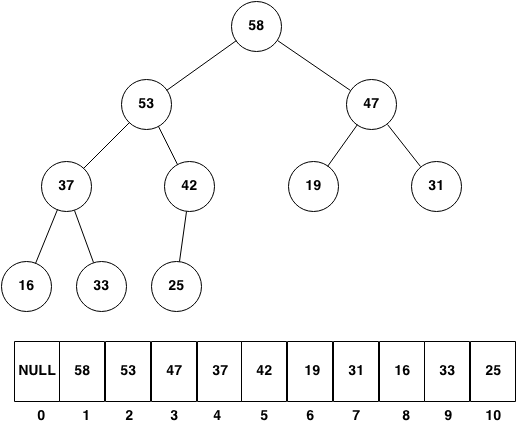
\includegraphics[width=100mm]{heap2.png}
\caption{Αναπαράσταση ενός σωρού μεγίστων ως πίνακα}
\label{fig:heap2}
\end{figure}

Για το παράδειγμα του σχήματος ισχύουν τα ακόλουθα:
\begin{itemize}
\item Οι κόμβοι που είναι γονείς (έχουν τουλάχιστον ένα παιδί) βρίσκονται στις θέσεις από 1 μέχρι και 5.
\item Οι κόμβοι που είναι φύλλα βρίσκονται στις θέσεις από 6 μέχρι και 10.
\item Ο γονέας στη θέση 1 (η τιμή 58) έχει παιδιά στις θέσεις $2*1=2$ (τιμή 53) και $2*1+1=3$ (τιμή 47).
\item Ο γονέας στη θέση 2 (η τιμή 53) έχει παιδιά στις θέσεις $2*2=4$ (τιμή 37) και $2*2+1=5$ (τιμή 42).
\item Ο γονέας στη θέση 3 (η τιμή 47) έχει παιδιά στις θέσεις $2*3=6$ (τιμή 19) και $2*3+1=7$ (τιμή 31).
\item Ο γονέας στη θέση 4 (η τιμή 37) έχει παιδιά στις θέσεις $2*4=8$ (τιμή 16) και $2*4+1=9$ (τιμή 33).
\item Ο γονέας στη θέση 5 (η τιμή 42) έχει παιδιά στις θέσεις $2*5=10$ (τιμή 25).
\item Ο κόμβος παιδί στη θέση 2 (η τιμή 53) έχει γονέα στη θέση $\lfloor{\frac{2}{2}}\rfloor=1$ (τιμή 58).
\item Ο κόμβος παιδί στη θέση 3 (η τιμή 47) έχει γονέα στη θέση $\lfloor{\frac{3}{2}}\rfloor=1$ (τιμή 58).
\item Ο κόμβος παιδί στη θέση 4 (η τιμή 37) έχει γονέα στη θέση $\lfloor{\frac{4}{2}}\rfloor=2$ (τιμή 53).
\item Ο κόμβος παιδί στη θέση 5 (η τιμή 42) έχει γονέα στη θέση $\lfloor{\frac{5}{2}}\rfloor=2$ (τιμή 53).
\item Ο κόμβος παιδί στη θέση 6 (η τιμή 19) έχει γονέα στη θέση $\lfloor{\frac{6}{2}}\rfloor=3$ (τιμή 47).
\item Ο κόμβος παιδί στη θέση 7 (η τιμή 31) έχει γονέα στη θέση $\lfloor{\frac{7}{2}}\rfloor=3$ (τιμή 47).
\item Ο κόμβος παιδί στη θέση 8 (η τιμή 16) έχει γονέα στη θέση $\lfloor{\frac{8}{2}}\rfloor=4$ (τιμή 37).
\item Ο κόμβος παιδί στη θέση 9 (η τιμή 33) έχει γονέα στη θέση $\lfloor{\frac{9}{2}}\rfloor=4$ (τιμή 37).
\item Ο κόμβος παιδί στη θέση 10 (η τιμή 25) έχει γονέα στη θέση $\lfloor{\frac{10}{2}}\rfloor=5$ (τιμή 42).
\end{itemize}

\section{Υλοποίηση ενός σωρού}
Στη συνέχεια παρουσιάζεται η υλοποίηση ενός σωρού μεγίστων που περιέχει ακέραιες τιμές-κλειδιά.

\lstinputlisting[caption = Σωρός μεγίστων με κλειδιά ακέραιες τιμές (max\_heap.cpp)]{lab06/max_heap.cpp}

\subsubsection*{Οι συναρτήσεις δημιουργίας σωρού από πίνακα (heap\_bottom\_up και heapify)}
Ένας πίνακας μπορεί να μετασχηματιστεί ταχύτατα σε σωρό. Η διαδικασία ξεκινά από τον τελευταίο κόμβο γονέα του δένδρου (που βρίσκεται στη θέση $\lfloor{\frac{n}{2}}\rfloor$) και σταδιακά εφαρμόζεται μέχρι να φτάσει στον κόμβο στη θέση 1. Για καθένα από αυτούς τους κόμβους εξετάζεται από πάνω προς τα κάτω αν ισχύει η κυριαρχία γονέα και αν δεν ισχύει τότε γίνεται αντιμετάθεση με το μεγαλύτερο από τα παιδιά του επαναληπτικά. 

Ο ακόλουθος κώδικας χρησιμοποιεί τη συνάρτηση heap\_bottom\_up και μέσω αυτής τη συνάρτηση heapify προκειμένου να μετασχηματίσει έναν πίνακα ακεραίων σε σωρό μεγίστων. 
\lstinputlisting[caption = Δημιουργία σωρού από πίνακα με heapify (heap1.cpp)]{lab06/heap1.cpp}

\lstinputlisting[style=DOS]{lab06/heap1.out}

Στο σχήμα \ref{fig:heapify} παρουσιάζονται οι τιμές που έλαβε κάθε κόμβος του δένδρου προκειμένου να μετασχηματιστεί τελικά σε σωρό μεγίστων.

\begin{figure}[ht]
\centering
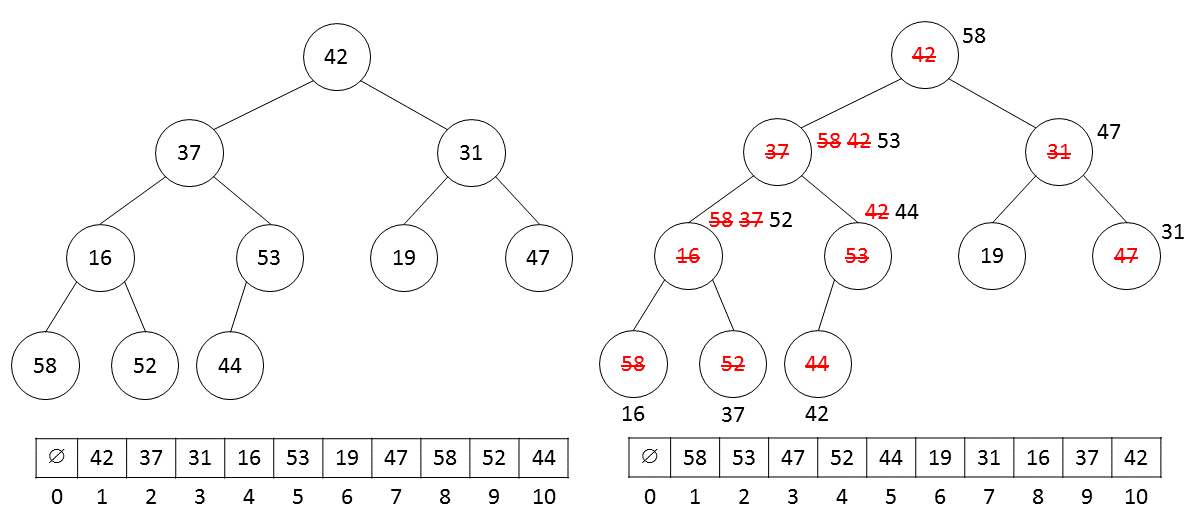
\includegraphics[width=150mm]{heapify.png}
\caption{Δημιουργία σωρού από πίνακα (heapify)}
\label{fig:heapify}
\end{figure}

\subsubsection*{Η συνάρτηση ελέγχου του εάν ο σωρός είναι άδειος (empty)}
Η συνάρτηση empty εξετάζει το μέγεθος του σωρού μέσω της μεταβλητής heap\_size. Αν η μεταβλητή heap\_size είναι μηδέν τότε επιστρέφει true, αλλιώς επιστρέφει false.

\subsubsection*{Η συνάρτηση λήψης της μεγαλύτερης τιμής από το σωρό (top)}
Καθώς η μεγαλύτερη τιμή βρίσκεται πάντα στη θέση 1 του πίνακα που διατηρεί τα δεδομένα του σωρού η συνάρτηση top απλά επιστρέφει την τιμή αυτή.

\subsubsection*{Η συνάρτηση εξαγωγής της μεγαλύτερης τιμής από το σωρό (pop)}
Η εξαγωγή της μεγαλύτερης τιμής γίνεται ως εξής. Το στοιχείο που βρίσκεται στην κορυφή του σωρού αντιμετατίθεται με το τελευταίο στοιχείο του σωρού. Στη συνέχεια το στοιχείο που έχει βρεθεί στην κορυφή του σωρού κατεβαίνει προς τα κάτω αν έχει παιδί που είναι μεγαλύτερό του πραγματοποιώντας αντιμετάθεση με το μεγαλύτερο στοιχείο από τα παιδιά του. Η διαδικασία επαναλαμβάνεται για τη νέα θέση του στοιχείου που αρχικά είχε μεταφερθεί στη κορυφή και μέχρι να ισχύσει ότι είναι μεγαλύτερο και από τα δύο παιδιά του. Στο σχήμα \ref{fig:heap_pop} παρουσιάζεται η εξαγωγή της κορυφαίας τιμής του σωρού.

\begin{figure}[ht!]
\centering
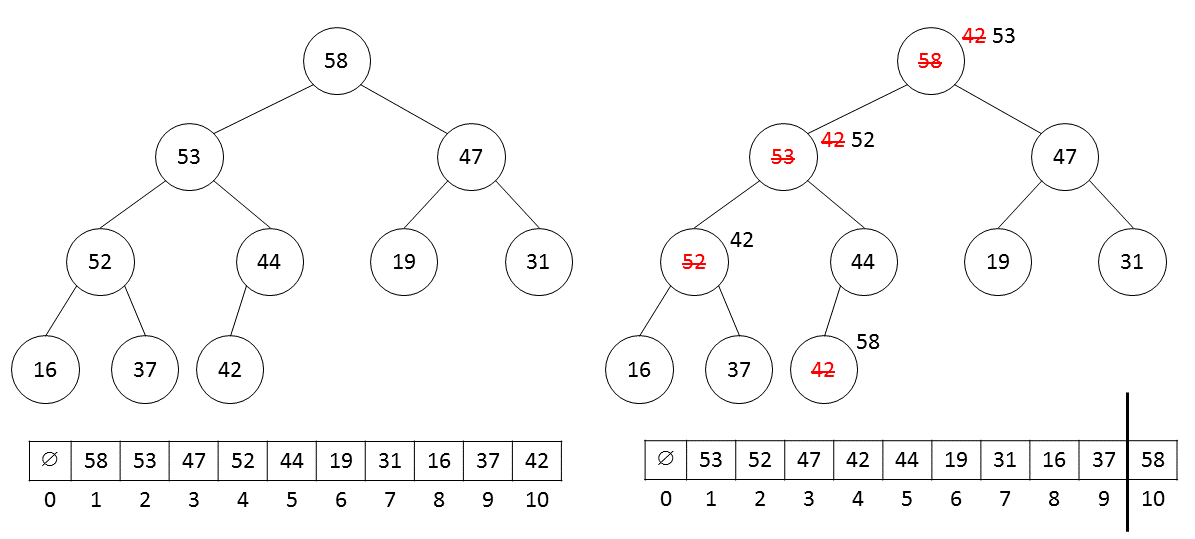
\includegraphics[width=150mm]{heap_pop.png}
\caption{Εξαγωγή της μεγαλύτερης τιμής του σωρού (pop)}
\label{fig:heap_pop}
\end{figure}

\subsubsection*{Η συνάρτηση εισαγωγής νέας τιμής στο σωρό (push)}
Η εισαγωγή ενός στοιχείου γίνεται ως φύλλο στη πρώτη διαθέσιμη θέση από πάνω προς τα κάτω και από δεξιά προς τα αριστερά. Το στοιχείο αυτό συγκρίνεται με το γονέα του και αν είναι μεγαλύτερο αντιμετατίθεται με αυτόν. Η διαδικασία συνεχίζεται μέχρι είτε να βρεθεί το νέο στοιχείο στην κορυφή είτε να ισχύει η κυριαρχία γονέα. Στο σχήμα \ref{fig:heap_push} παρουσιάζεται η εισαγωγή της τιμής 60 σε έναν σωρό μεγίστων.

\begin{figure}[H]
\centering
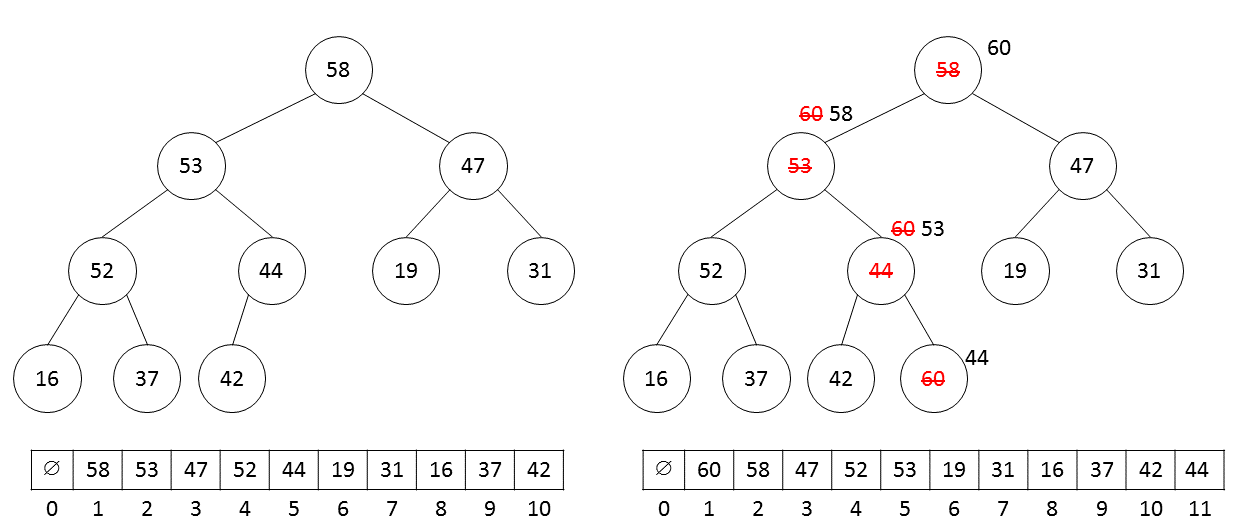
\includegraphics[width=150mm]{heap_push.png}
\caption{Εισαγωγή της τιμής 60 στο σωρό (push)}
\label{fig:heap_push}
\end{figure}


\subsubsection*{Παράδειγμα χρήσης των συναρτήσεων push και pop)}
Ο ακόλουθος κώδικας δημιουργεί σταδιακά έναν σωρό εισάγοντας δέκα τιμές με τη συνάρτηση push. Στη συνέχεια πραγματοποιούνται εξαγωγές τιμών με τη συνάρτηση pop μέχρι ο σωρός να αδειάσει.

\lstinputlisting[caption = Δημιουργία σωρού με εισαγωγές τιμών και εν συνεχεία άδειασμα του σωρού με διαδοχικές διαγραφές της μέγιστης τιμής (heap2.cpp)]{lab06/heap2.cpp}

\lstinputlisting[style=DOS]{lab06/heap2.out}


\section{Ταξινόμηση Heapsort}
Ο αλγόριθμος Heapsort προτάθηκε από τον J.W.J.Williams το 1964 \cite{nist_heapsort} και αποτελείται από 2 στάδια:
\begin{itemize}[noitemsep]
\item Δημιουργία σωρού με τα n στοιχεία ενός πίνακα που ζητείται να ταξινομηθούν. 
\item Εφαρμογή της διαγραφής της ρίζας n -1 φορές.
\end{itemize}
Το αποτέλεσμα είναι ότι τα στοιχεία αφαιρούνται από το σωρό σε φθίνουσα σειρά (για έναν σωρό μεγίστων). Καθώς κατά την αφαίρεσή του κάθε στοιχείου, αυτό τοποθετείται στο τέλος του σωρού, τελικά ο σωρός περιέχει τα αρχικά δεδομένα σε αύξουσα σειρά. 

Στη συνέχεια παρουσιάζεται η υλοποίηση του αλγορίθμου Heapsort. Επιπλέον ο κώδικας ταξινομεί πίνακες μεγέθους 10.000, 20.000, 40.000 80.000 και 100.000 που περιέχουν τυχαίες ακέραιες τιμές και πραγματοποιείται σύγκριση με τους χρόνους εκτέλεσης που επιτυγχάνει η std::sort.

\lstinputlisting[caption = Ο αλγόριθμος heapsort (heapsort.cpp)]{lab06/heapsort.cpp}

\lstinputlisting[style=DOS]{lab06/heapsort.out}

Περισσότερες πληροφορίες για την ταξινόμηση heapsort μπορούν να βρεθούν στην αναφορά \cite{programiz_heapsort}.


\section{Η δομή priority\_queue της STL}
Η STL της C++ περιέχει υλοποίηση της δομής std::priority\_queue (ουρά προτεραιότητας) η οποία είναι ένας σωρός μεγίστων. Κάθε στοιχείο που εισέρχεται  στην ουρά προτεραιότητας έχει μια προτεραιότητα που συνδέεται με αυτό και το στοιχείο με τη μεγαλύτερη προτεραιότητα βρίσκεται πάντα στην αρχή της ουράς. Οι κυριότερες λειτουργίες που υποστηρίζονται από την std::priority\_queue είναι οι ακόλουθες:
\begin{itemize}[noitemsep]
\item push: εισαγωγή ενός στοιχείου στη δομή.
\item top: επιστροφή χωρίς εξαγωγή του στοιχείου με τη μεγαλύτερη προτεραιότητα.
\item pop: απώθηση του στοιχείου με τη μεγαλύτερη προτεραιότητα.
\item size: πλήθος των στοιχείων που υπάρχουν στη δομή.
\item empty: επιστρέφει true αν η δομή είναι άδεια αλλιώς επιστρέφει false.
\end{itemize}
Ένα παράδειγμα χρήσης της std::priority\_queue ως σωρού μεγίστων αλλά και ως σωρού ελαχίστων παρουσιάζεται στη συνέχεια.

\lstinputlisting[caption = Παράδειγμα με priority\_queue της STL (stl\_priority\_queue.cpp)]{lab06/stl_priority_queue.cpp}

\lstinputlisting[style=DOS]{lab06/stl_priority_queue.out}

Περισσότερες πληροφορίες για τη δομή std::priority\_queue μπορούν να βρεθούν στις αναφορές \cite{g4g_priority_queue} και \cite{cppref_priority_queue}.


\section{Παραδείγματα}
\subsection{Παράδειγμα 1}
Χρησιμοποιώντας τον κώδικα 1, να γραφεί πρόγραμμα που να εισάγει 100.000 τυχαίες ακέραιες τιμές (στο διάστημα [-1.000.000,1.000.000]) σε έναν σωρό μεγίστων με τη συνάρτηση heap\_bottom\_up καθώς και με διαδοχικές κλήσεις της συνάρτησης push. Χρονομετρείστε τον κώδικα και στις δύο περιπτώσεις δημιουργίας του σωρού και εμφανίστε το κορυφαίο στοιχείο του σωρού. Επαναλάβετε τη διαδικασία χρησιμοποιώντας την std::priority\_queue.

\lstinputlisting[caption = Χρόνος δημιουργίας MAXHEAP: Α) με την heap\_bottom\_up Β) με σταδιακές εισαγωγές (push) τιμών στο σωρό και C) με την std::priority\_queue (lab06\_ex1.cpp)]{lab06/lab06_ex1.cpp}

\lstinputlisting[style=DOS]{lab06/lab06_ex1.out}

\subsection{Παράδειγμα 2}
Έστω ένα παιχνίδι στο οποίο οι παίκτες έχουν όνομα (name) και επίδοση (score). Να γράψετε πρόγραμμα στο οποίο να εισέρχονται στο παιχνίδι 10 παίκτες στη σειρά (player1, player2, ...), πετυχαίνοντας κάποια επίδοση ο καθένας (τυχαίος ακέραιος από το 0 μέχρι το 50.000). Να εμφανίζεται μετά την εισαγωγή του κάθε παίκτη ο παίκτης που προηγείται και η επίδοση του. Τέλος, να εμφανίζονται τα ονόματα των παικτών με τις 3 υψηλότερες επιδόσεις.

\lstinputlisting[caption = Διατήρηση επιδόσεων σε σωρό (lab06\_ex2.cpp)]{lab06/lab06_ex2.cpp}

\lstinputlisting[style=DOS]{lab06/lab06_ex2.out}


\subsection{Παράδειγμα 3}
Διάμεσος ενός δείγματος Ν παρατηρήσεων οι οποίες έχουν διαταχθεί σε αύξουσα σειρά ορίζεται ως η μεσαία παρατήρηση, όταν το Ν είναι περιττός αριθμός, ή ο μέσος όρος (ημιάθροισμα) των δύο μεσαίων παρατηρήσεων όταν το Ν είναι άρτιος αριθμός. 
Έστω ότι για διάφορες τιμές που παράγονται με κάποιον τρόπο ζητείται ο υπολογισμός της διάμεσης  τιμής καθώς παράγεται κάθε νέα τιμή και για όλες τις τιμές που έχουν προηγηθεί μαζί με την τρέχουσα τιμή όπως φαίνεται στο επόμενο παράδειγμα:\\ 
5  $\Rightarrow$  διάμεσος 5\\
5, 7 $\Rightarrow$ διάμεσος 6\\
5, 7, 13 $\Rightarrow$ διάμεσος 7\\
5, 7, 13, 12 $\Rightarrow$ 5, 7, 12, 13 $\Rightarrow$ διάμεσος 9.5\\
5, 7, 13, 12, 2 $\Rightarrow$ 2, 5, 7, 12, 13 $\Rightarrow$ διάμεσος 7

\lstinputlisting[caption = Υπολογισμός διαμέσου σε μια ροή τιμών (lab06\_ex3.cpp)]{lab06/lab06_ex3.cpp}

\lstinputlisting[style=DOS]{lab06/lab06_ex3.out}


\section{Ασκήσεις}
\begin{enumerate}
\item Να υλοποιηθεί ο σωρός μεγίστων που παρουσιάστηκε στον κώδικα 1 ως κλάση. Προσθέστε εξαιρέσεις έτσι ώστε να χειρίζονται περιπτώσεις όπως όταν ο σωρός είναι άδειος και ζητείται εξαγωγή της μεγαλύτερης τιμής ή όταν ο σωρός είναι γεμάτος και επιχειρείται εισαγωγή νέας τιμής.
\item Να γραφεί συνάρτηση που να δέχεται ως παράμετρο έναν πίνακα ακεραίων και έναν ακέραιο αριθμό κ και να επιστρέφει το κ-οστό μεγαλύτερο στοιχείο του πίνακα. 
%\item b
%\item d
\end{enumerate}

\begin{thebibliography}{9}
\bibitem{nist_heapsort}
NIST, heapsort, \href{https://xlinux.nist.gov/dads/HTML/heapSort.html}{https://xlinux.nist.gov/dads/HTML/heapSort.html}

\bibitem{programiz_heapsort}
PROGRAMIZ, Heap Sort Algorithm, \href{https://www.programiz.com/dsa/heap-sort}{https://www.programiz.com/dsa/heap-sort}

\bibitem{g4g_priority_queue}
Geeks for Geeks, Priority Queue in C++ Standard Template Library (STL), \href{http://www.geeksforgeeks.org/priority-queue-in-cpp-stl/}{http://www.geeksforgeeks.org/priority-queue-in-cpp-stl/}

\bibitem{cppref_priority_queue}
Cppreference.com, std::priority\_queue, \href{http://en.cppreference.com/w/cpp/container/priority_queue}{http://en.cppreference.com/w/cpp/container/priority\_queue}

\end{thebibliography}



% Εργαστήριο 7
\chapter{Κατακερματισμός, δομές κατακερματισμού στην STL}
\chaptermark{Κατακερματισμός}
\section{Εισαγωγή}
Ο κατακερματισμός (hashing) αποτελεί μια από τις βασικές τεχνικές στη επιστήμη των υπολογιστών. Χρησιμοποιείται στις δομές δεδομένων αλλά και σε άλλα πεδία της πληροφορικής όπως η κρυπτογραφία. Στο εργαστήριο αυτό θα παρουσιαστεί η δομή δεδομένων πίνακας κατακερματισμού χρησιμοποιώντας δύο διαδεδομένες υλοποιήσεις: την ανοικτή διευθυνσιοδότηση και την υλοποίηση με αλυσίδες. Επιπλέον, θα παρουσιαστούν δομές της STL όπως η unordered\_set και η unordered\_map οι οποίες στηρίζονται στην τεχνική του κατακερματισμού. Ο κώδικας όλων των παραδειγμάτων, όπως και στα προηγούμενα εργαστήρια, βρίσκεται στο \href{https://github.com/chgogos/ceteiep_dsa}{https://github.com/chgogos/ceteiep\_dsa}.

\section{Τι είναι ο κατακερματισμός;}
Ο κατακερματισμός είναι μια μέθοδος που επιτυγχάνει ταχύτατη αποθήκευση, αναζήτηση και διαγραφή δεδομένων. Σε ένα σύστημα κατακερματισμού τα δεδομένα αποθηκεύονται σε έναν πίνακα που ονομάζεται πίνακας κατακερματισμού (hash table). Θεωρώντας ότι τα δεδομένα είναι εγγραφές που αποτελούνται από ζεύγη τιμών της μορφής κλειδί-τιμή, η βασική ιδέα είναι, ότι εφαρμόζοντας στο κλειδί κάθε εγγραφής που πρόκειται να αποθηκευτεί ή να αναζητηθεί τη λεγόμενη συνάρτηση κατακερματισμού (hash function), προσδιορίζεται μονοσήμαντα η θέση του πίνακα στην οποία τοποθετούνται τα δεδομένα της εγγραφής. Η συνάρτηση κατακερματισμού αναλαμβάνει να αντιστοιχήσει έναν μεγάλο αριθμό ή ένα λεκτικό σε ένα μικρό ακέραιο που χρησιμοποιείται ως δείκτης στον πίνακα κατακερματισμού.

\begin{figure}[ht]
\centering
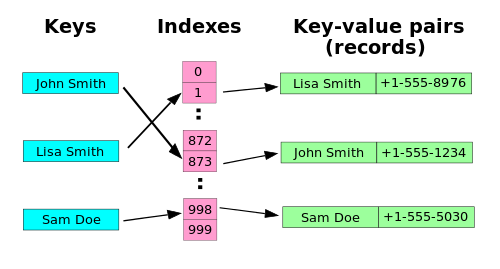
\includegraphics[width=100mm]{HASHTB08.png}
\caption{Κατακερματισμός εγγραφών σε πίνακα κατακερματισμού \cite{wiki_hashtables}}
\label{fig:hashtable1}
\end{figure}

Μια καλή συνάρτηση κατακερματισμού θα πρέπει να κατανέμει τα κλειδιά στα κελιά του πίνακα κατακερματισμού όσο πιο ομοιόμορφα γίνεται και να είναι εύκολο να υπολογιστεί. Επίσης, είναι επιθυμητό το παραγόμενο αποτέλεσμα από τη συνάρτηση κατακερματισμού να εξαρτάται από το κλειδί στο σύνολό του.

Στον κώδικα που ακολουθεί παρουσιάζονται τέσσερις συναρτήσεις κατακερματισμού κάθε μία από τις οποίες δέχεται ένα λεκτικό και επιστρέφει έναν ακέραιο αριθμό. Στις συναρτήσεις hash2 και hash3 γίνεται χρήση τελεστών που εφαρμόζονται σε δυαδικές τιμές (bitwise operators). Ειδικότερα χρησιμοποιούνται οι τελεστές $<<$ (αριστερή ολίσθηση), $>>$ (δεξιά ολίσθηση) και $\hat{}$ (xor - αποκλειστικό ή).

\lstinputlisting[caption = Διάφορες συναρτήσεις κατακερματισμού (hashes.cpp)]{lab07/hashes.cpp}

\lstinputlisting[caption = Παραδείγματα κλήσεων συναρτήσεων κατακερματισμού (hashes\_ex1.cpp)]{lab07/hashes_ex1.cpp}

\lstinputlisting[style=DOS]{lab07/hashes_ex1.out}


Οι πίνακες κατακερματισμού είναι ιδιαίτερα κατάλληλοι για εφαρμογές στις οποίες πραγματοποιούνται συχνές αναζητήσεις εγγραφών με δεδομένες τιμές κλειδιών. Οι βασικές λειτουργίες που υποστηρίζονται σε έναν πίνακα κατακερματισμού είναι η εισαγωγή (insert), η αναζήτηση (get) και η διαγραφή (erase). Και οι τρεις αυτές λειτουργίες παρέχονται σε χρόνο $O(1)$ κατά μέσο όρο προσφέροντας ταχύτερη υλοποίηση σε σχέση με άλλες υλοποιήσεις όπως για παράδειγμα τα ισοζυγισμένα δυαδικά δένδρα αναζήτησης που παρέχουν τις ίδιες λειτουργίες σε χρόνο $O(log n)$. 

Ωστόσο, οι πίνακες κατακερματισμού έχουν και μειονεκτήματα καθώς είναι δύσκολο να επεκταθούν από τη στιγμή που έχουν δημιουργηθεί και μετά. Επίσης, η απόδοση των πινάκων κατακερματισμού υποβαθμίζεται καθώς οι θέσεις τους γεμίζουν με στοιχεία. Συνεπώς, εφόσον ο προγραμματιστής προχωρήσει στη δική του υλοποίηση ενός πίνακα κατακερματισμού είτε θα πρέπει να γνωρίζει εκ των προτέρων το πλήθος των στοιχείων που πρόκειται να αποθηκευτούν είτε όταν αυτό απαιτηθεί να υπάρχει πρόβλεψη έτσι ώστε τα δεδομένα να μεταφέρονται σε μεγαλύτερο πίνακα κατακερματισμού.

Στις περισσότερες εφαρμογές υπάρχουν πολύ περισσότερα πιθανά κλειδιά εγγραφών από ότι θέσεις στο πίνακα κατακερματισμού. Αν για δύο ή περισσότερα κλειδιά η εφαρμογή της συνάρτησης κατακερματισμού επιστρέφει το ίδιο αποτέλεσμα τότε λέμε ότι συμβαίνει σύγκρουση (collision) η οποία θα πρέπει να διευθετηθεί με κάποιο τρόπο. Ο ακόλουθος κώδικας μετρά το πλήθος των συγκρούσεων που συμβαίνουν καθώς δημιουργούνται hashes για ένα σύνολο 2.000 κλειδιών αλφαριθμητικού τύπου.


\lstinputlisting[caption = Δημιουργία τυχαίων λεκτικών (random\_strings.cpp)]{lab07/random_strings.cpp}

\lstinputlisting[caption = Συγκρούσεις (hashes\_ex2.cpp)]{lab07/hashes_ex2.cpp}

\lstinputlisting[style=DOS]{lab07/hashes_ex2.out}

Γενικότερα, σε έναν πίνακα κατακερματισμού, η εύρεση μιας εγγραφής με κλειδί key είναι μια διαδικασία δύο βημάτων:
\begin{itemize}[noitemsep]
\item Εφαρμογή της συνάρτησης κατακερματισμού στο κλειδί της εγγραφής.
\item Ξεκινώντας από την θέση που υποδεικνύει η συνάρτηση κατακερματισμού στον πίνακα κατακερματισμού, εντοπισμός της εγγραφής που περιέχει το ζητούμενο κλειδί (ενδεχόμενα θα χρειαστεί να εφαρμοστεί κάποιος μηχανισμός διευθέτησης συγκρούσεων). 
\end{itemize}

Οι βασικοί μηχανισμοί επίλυσης των συγκρούσεων είναι η ανοικτή διευθυνσιοδότηση και ο κατακερματισμός με αλυσίδες.

\subsection{Ανοικτή διευθυνσιοδότηση}
Στην ανοικτή διευθυνσιοδότηση (open addressing, closed hashing) όλα τα δεδομένα αποθηκεύονται απευθείας στον πίνακα κατακερματισμού. Αν συμβεί σύγκρουση τότε ελέγχεται αν κάποιο από τα υπόλοιπα κελιά είναι διαθέσιμο και η εγγραφή τοποθετείται εκεί. Συνεπώς, θα πρέπει το μέγεθος του hashtable να είναι μεγαλύτερο ή ίσο από το πλήθος των στοιχείων που πρόκειται να αποθηκευτούν σε αυτό. Θα πρέπει να σημειωθεί ότι η απόδοση της ανοικτής διευθυνσιοδότησης μειώνεται κατακόρυφα σε περίπτωση που το hashtable είναι σχεδόν γεμάτο. 

Αν το πλήθος των κελιών είναι $m$ και το πλήθος των εγγραφών είναι $n$ τότε το πηλίκο $a=\frac{n}{m}$ που ονομάζεται παράγοντας φόρτωσης (load factor) καθορίζει σημαντικά την απόδοση του hashtable. Ο παράγοντας φόρτωσης στην περίπτωση της ανοικτής διευθυνσιοδότησης δεν μπορεί να είναι μεγαλύτερος της μονάδας.

Υπάρχουν πολλές παραλλαγές της ανοικτής διευθυνσιοδότησης που σχετίζονται με τον τρόπο που σε περίπτωση σύγκρουσης επιλέγεται το επόμενο κελί που εξετάζεται αν είναι ελεύθερο προκειμένου να τοποθετηθούν εκεί τα δεδομένα της εγγραφής. Αν εξετάζεται το αμέσως επόμενο στη σειρά κελί και μέχρι να βρεθεί το πρώτο διαθέσιμο, ξεκινώντας από την αρχή του πίνακα αν βρεθεί στο τέλος, τότε η μέθοδος ονομάζεται γραμμική ανίχνευση (linear probing). Άλλες διαδεδομένες μέθοδοι είναι η τετραγωνική ανίχνευση (quadratic probing) και ο διπλός κατακερματισμός (double hashing) \cite{visualalgo_hashtables}.

\begin{figure}[ht]
\centering
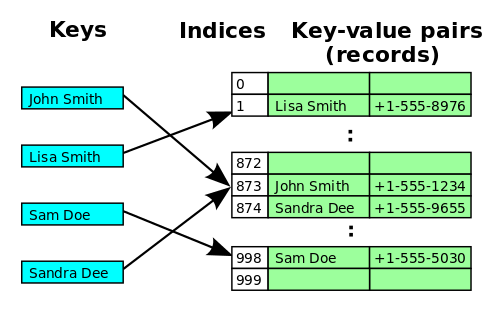
\includegraphics[width=100mm]{HASHTB12.png}
\caption{Κατακερματισμός εγγραφών με ανοικτή διευθυνσιοδότηση και γραμμική ανίχνευση \cite{wiki_hashtables}}
\label{fig:hashtable2}
\end{figure}

Στη συνέχεια ακολουθεί μια υλοποίηση ενός πίνακα κατακερματισμού με ανοικτή διευθυνσιοδότηση και γραμμική ανίχνευση. Στον πίνακα κατακερματισμού τοποθετούνται εγγραφές με κλειδιά και τιμές αλφαριθμητικού τύπου. 

\lstinputlisting[label={lst:open_addressing},caption={Ανοικτή διευθυνσιοδότηση (open\_addressing.cpp)}]{lab07/open_addressing.cpp}

\lstinputlisting[style=DOS]{lab07/open_addressing.out}

\subsection{Κατακερματισμός με αλυσίδες}
Στον κατακερματισμό με αλυσίδες (separate chaining) οι εγγραφές αποθηκεύονται σε συνδεδεμένες λίστες κάθε μια από τις οποίες είναι προσαρτημένες στα κελιά ενός hashtable. Συνεπώς, η απόδοση των αναζητήσεων εξαρτάται από τα μήκη των συνδεδεμένων λιστών. Αν η συνάρτηση κατακερματισμού κατανέμει τα $n$ κλειδιά ανάμεσα στα $m$ κελιά ομοιόμορφα τότε κάθε λίστα θα έχει μήκος $\frac{n}{m}$. O παράγοντας φόρτωσης, $a=\frac{n}{m}$, στον κατακερματισμό με αλυσίδες δεν θα πρέπει να απέχει πολύ από την μονάδα. Πολύ μικρό load factor σημαίνει ότι υπάρχουν πολλές κενές λίστες και συνεπώς δεν γίνεται αποδοτική χρήση του χώρου ενώ μεγάλο load factor σημαίνει μακριές συνδεδεμένες λίστες και μεγαλύτεροι χρόνοι αναζήτησης. 

\begin{figure}[ht]
\centering
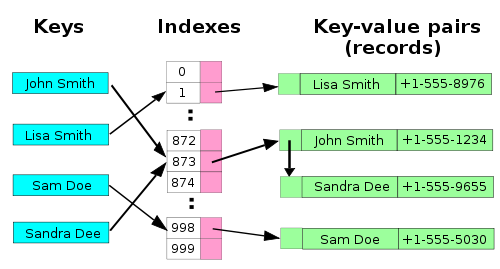
\includegraphics[width=100mm]{HASHTB32.png}
\caption{Κατακερματισμός εγγραφών με αλυσίδες \cite{wiki_hashtables}}
\label{fig:hashtable3}
\end{figure}

Στη συνέχεια ακολουθεί μια υλοποίηση ενός πίνακα κατακερματισμού με κατακερματισμό με αλυσίδες. Για τις συνδεδεμένες λίστες χρησιμοποιείται η λίστα std::list.

\lstinputlisting[caption = Κατακερματισμός με αλυσίδες (separate\_chaining.cpp)]{lab07/separate_chaining.cpp}

\lstinputlisting[style=DOS]{lab07/separate_chaining.out}

Περισσότερες πληροφορίες σχετικά με τον κατακερματισμό και την υλοποίηση πινάκων κατακερματισμού μπορούν να βρεθούν στις αναφορές \cite{pumpkin_hashtables}, \cite{hackerearth_hashtables}.

\section{Κατακερματισμός με την STL}
Η STL διαθέτει την κλάση std::hash που μπορεί να χρησιμοποιηθεί για την επιστροφή hash τιμών για διάφορους τύπους δεδομένων. Στον ακόλουθο κώδικα παρουσιάζεται η χρήση της std::hash.

\lstinputlisting[caption = Παράδειγμα χρήσης της std::hash (stl\_hash.cpp)]{lab07/stl_hash.cpp}

\lstinputlisting[style=DOS]{lab07/stl_hash.out}
 

Επιπλέον, η STL υποστηρίζει δύο βασικές δομές κατακερματισμού το std::unordered\_set και το std::unordered\_map. Το std::unordered\_set υλοποιείται ως ένας πίνακας κατακερματισμού και μπορεί να περιέχει τιμές (κλειδιά) οποιουδήποτε τύπου οι οποίες γίνονται hash σε διάφορες θέσεις του πίνακα κατακερματισμού. Κατά μέσο όρο, οι λειτουργίες σε ένα std::unordered\_set (εύρεση, εισαγωγή και διαγραφή κλειδιού) πραγματοποιούνται σε σταθερό χρόνο O(1). Ένα std::unordered\_set δεν περιέχει διπλότυπα, ενώ αν υπάρχει αυτή η ανάγκη τότε μπορεί να χρησιμοποιηθεί το std::unordered\_multiset. 

Στον κώδικα που ακολουθεί οι χαρακτήρες ενός λεκτικού εισάγονται ένας προς ένας σε ένα std::unordered\_set έτσι ώστε να υπολογιστεί το πλήθος των διακριτών χαρακτήρων ενός λεκτικού.

\lstinputlisting[caption = Παράδειγμα χρήσης του std::unordered\_set (stl\_unordered\_set.cpp)]{lab07/stl_unordered_set.cpp}

\lstinputlisting[style=DOS]{lab07/stl_unordered_set.out}

To std::unordered\_map αποθηκεύει ζεύγη (κλειδί-τιμή). Το κλειδί αναγνωριζει με μοναδικό τρόπο το κάθε ζεύγος και γίνεται hash σε συγκεκριμένη θέση του πίνακα κατακερματισμού. Όπως και στο std::unordered\_set. κατά μέσο όρο, οι λειτουργίες σε ένα std::unordered\_map πραγματοποιούνται σε σταθερό χρόνο O(1). Η ανάθεση τιμής σε κλειδί μπορεί να γίνει με τους τελεστές = και [], ενώ το πέρασμα από τις τιμές ενός std::unordered\_map μπορεί να γίνει με  iterator ή με range for.
 
\lstinputlisting[caption = Παράδειγμα χρήσης του std::unordered\_map (stl\_unordered\_map.cpp)]{lab07/stl_unordered_map.cpp}

\lstinputlisting[style=DOS]{lab07/stl_unordered_map.out}

%\section{Κατακερματισμός και κρυπτογράφηση}
%
%\section{Bloom filters}
%A Bloom filter is a space-efficient probabilistic data structure, conceived by Burton Howard Bloom in 1970, that is used to test whether an element is a member of a set. False positive matches are possible, but false negatives are not – in other words, a query returns either "possibly in set" or "definitely not in set". Elements can be added to the set, but not removed (though this can be addressed with a "counting" filter); the more elements that are added to the set, the larger the probability of false positives.

\section{Παραδείγματα}

\subsection{Παράδειγμα 1}
Έστω μια επιχείρηση η οποία επιθυμεί να αποθηκεύσει τα στοιχεία των υπαλλήλων της (όνομα, διεύθυνση) σε μια δομή έτσι ώστε με βάση το όνομα του υπαλλήλου να επιτυγχάνει τη γρήγορη ανάκληση των υπόλοιπων στοιχείων των υπαλλήλων. Στη συνέχεια παρουσιάζεται η υλοποίηση ενός πίνακα κατακερματισμού στον οποίο κλειδί θεωρείται το όνομα του υπαλλήλου και η επίλυση των συγκρούσεων πραγματοποιείται με ανοικτή διευθυνσιοδότηση (open addressing) και γραμμική ανίχνευση (linear probing). Καθώς δεν υπάρχει η ανάγκη διαγραφής τιμών από τον πίνακα κατακερματισμού παρουσιάζεται μια απλούστερη υλοποίηση σε σχέση με αυτή που παρουσιάστηκε στον κώδικα \ref{lst:open_addressing}. Ο πίνακας κατακερματισμού μπορεί να δεχθεί το πολύ 100.000 εγγραφές υπαλλήλων. Στο παράδειγμα χρονομετρείται η εκτέλεση για 20.000, 30.000 και 80.000 υπαλλήλους. Παρατηρείται ότι λόγω των συγκρούσεων καθώς ο συντελεστής φόρτωσης του πίνακα κατακερματισμού αυξάνεται η απόδοση της δομής υποβαθμίζεται.

\lstinputlisting[caption = Yλοποίηση πίνακα κατακερματισμού για γρήγορη αποθήκευση και αναζήτηση εγγραφών (lab07\_ex1.cpp)]{lab07/lab07_ex1.cpp}

\lstinputlisting[style=DOS]{lab07/lab07_ex1.out}

\subsection{Παράδειγμα 2}
Στο παράδειγμα αυτό παρουσιάζεται η λύση του ίδιου προβλήματος με το παράδειγμα 1 με τη διαφορά ότι πλέον χρησιμοποιείται η δομή std::unordered\_map της STL.

\lstinputlisting[caption = Γρήγορη αποθήκευση και αναζήτηση εγγραφών με τη χρήση της std::unordered\_map (lab07\_ex2.cpp)]{lab07/lab07_ex2.cpp}

\lstinputlisting[style=DOS]{lab07/lab07_ex2.out}

\subsection{Παράδειγμα 3}
Στο παράδειγμα αυτό εξετάζονται τέσσερις διαφορετικοί τρόποι με τους οποίους ελέγχεται για ένα μεγάλο πλήθος τιμών (5.000.000) πόσες από αυτές περιέχονται σε ένα δεδομένο σύνολο 1.000 τιμών. Οι τιμές είναι ακέραιες και επιλέγονται με τυχαίο τρόπο στο διάστημα [0,100.000]. Ο χρόνος που απαιτεί η κάθε προσέγγιση χρονομετρείται.
\begin{itemize}[noitemsep]
\item Η πρώτη προσέγγιση (scenario1) χρησιμοποιεί ένα vector για να αποθηκεύσει το σύνολο των 1.000 τυχαίων ακεραίων τιμών και αναζητά σειριακά κάθε τιμή στο vector. 
\item Η δεύτερη προσέγγιση (scenario2) χρησιμοποιεί επίσης ένα vector για να αποθηκεύσει το σύνολο των 1.000 τυχαίων ακεραίων τιμών, τις ταξινομεί και αναζητά κάθε τιμή στο ταξινομημένο vector. 
\item Η τρίτη προσέγγιση (scenario3) αποθηκεύει τις 1.000 τυχαίες ακεραίες τιμές σε ένα std::set (υλοποιείται στην STL ως δυαδικό δένδρο αναζήτησης) και αναζητά κάθε τιμή σε αυτό. 
\item Η τέταρτη προσέγγιση (scenario4) αποθηκεύει τις 1.000 τυχαίες ακεραίες τιμές σε ένα std::unordered\_set (υλοποιείται στην STL ως πίνακας κατακερματισμού) και αναζητά κάθε τιμή σε αυτό.
%\item Η πέμπτη προσέγγιση (scenario5) υλοποιεί ένα Bloom filter που χρησιμοποιεί ως βασική δομή ένα σύνολο δυαδικών ψηφίων με μέγεθος 10.001. 
\end{itemize}

\lstinputlisting[caption = Έλεγχος ύπαρξης τιμών σε ένα σύνολο τιμών (lab07\_ex3.cpp)]{lab07/lab07_ex3.cpp}

\lstinputlisting[style=DOS]{lab07/lab07_ex3.out}

\section{Ασκήσεις}
\begin{enumerate}
\item Γράψτε μια συνάρτηση που να δέχεται έναν πίνακα ακεραίων Α και έναν ακέραιο αριθμό sum και να βρίσκει το πλήθος από όλα τα ζεύγη τιμών του Α που το άθροισμά τους είναι ίσο με sum.
\item Γράψτε ένα πρόγραμμα που για ένα λεκτικό που θα δέχεται ως είσοδο, να επιστρέφει το χαρακτήρα (γράμματα κεφαλαία, γράμματα πεζά, ψηφία, σύμβολα) που εμφανίζεται περισσότερες φορές καθώς και πόσες φορές εμφανίζεται στο λεκτικό.
\item Γράψτε μια συνάρτηση που να δέχεται έναν πίνακα ακεραίων Α και έναν ακέραιο αριθμό Κ και να βρίσκει τη μεγαλύτερη σε μήκος υποακολουθία στοιχείων του Α που έχει άθροισμα ίσο με Κ.
\item Γράψτε ένα πρόγραμμα που να δέχεται μια λέξη και να βρίσκει γρήγορα όλες τις άλλες έγκυρες λέξεις που είναι αναγραμματισμοί της λέξης που δόθηκε. Θεωρείστε ότι έχετε δεδομένο ένα αρχείο κειμένου με όλες τις έγκυρες λέξεις (words.txt), μια ανά γραμμή.
\end{enumerate}

\begin{thebibliography}{9}
\bibitem{wiki_hashtables}
Wikibooks, Data Structures - Hash Tables \href{https://en.wikibooks.org/wiki/Data_Structures/Hash_Tables}{https://en.wikibooks.org/wiki/Data\_Structures/Hash\_Tables}

\bibitem{pumpkin_hashtables}
C++ tutorial: Intro to Hash Tables,
\href{https://pumpkinprogrammerdotcom4.wordpress.com/2014/06/21/c-tutorial-intro-to-hash-tables/}{https://pumpkinprogrammerdotcom4.wordpress.com/2014/06/21/c-tutorial-intro-to-hash-tables/}

\bibitem{hackerearth_hashtables}
HackerEarth, Basics of Hash Tables, \href{https://www.hackerearth.com/practice/data-structures/hash-tables/basics-of-hash-tables/tutorial/}{https://www.hackerearth.com/practice/data-structures/hash-tables/basics-of-hash-tables/tutorial/}

\bibitem{visualalgo_hashtables}
VisualAlgo.net Open Addressing (LP, QP, DH) and Separate Chaining Visualization, \href{https://visualgo.net/en/hashtable}{https://visualgo.net/en/hashtable}

\end{thebibliography}



% Εργαστήριο 8
\chapter{Γραφήματα}
\section{Εισαγωγή}
Τα γραφήματα είναι δομές δεδομένων που συναντώνται συχνά κατά την επίλυση προβλημάτων. Η ευχέρεια προγραμματισμού αλγορίθμων που εφαρμόζονται πάνω σε γραφήματα είναι ουσιώδης. Καθώς μάλιστα συχνά ανακύπτουν προβλήματα για τα οποία έχουν διατυπωθεί αλγόριθμοι αποδοτικής επίλυσής τους η γνώση των αλγορίθμων αυτών αποδεικνύεται ισχυρός σύμμαχος στην επίλυση δύσκολων προβλημάτων. 

\section{Γραφήματα}
Ένα γράφημα ή γράφος (graph) είναι ένα σύνολο από σημεία που ονομάζονται κορυφές (vertices) ή κόμβοι (nodes) για τα οποία ισχύει ότι κάποια από αυτά είναι συνδεδεμένα απευθείας μεταξύ τους με τμήματα γραμμών που ονομάζονται ακμές (edges ή arcs). Συνήθως ένα γράφημα συμβολίζεται ως $G=(V,E)$ όπου $V$ είναι το σύνολο των κορυφών και $E$ είναι το σύνολο των ακμών.

Αν οι ακμές δεν έχουν κατεύθυνση τότε το γράφημα ονομάζεται μη κατευθυνόμενο (undirected) ενώ σε άλλη περίπτωση ονομάζεται κατευθυνόμενο (directed). Ένα πλήρες γράφημα (που όλες οι κορυφές συνδέονται απευθείας με όλες τις άλλες κορυφές) έχει $\frac{|V||V-1|}{2}$ ακμές ($|V|$ είναι το πλήθος των κορυφών του γραφήματος). Αν σε κάθε ακμή αντιστοιχεί μια τιμή τότε το γράφημα λέγεται γράφημα με βάρη. Το γράφημα του σχήματος \ref{fig:undirected_graph1} είναι ένα μη κατευθυνόμενο γράφημα με βάρη. 

\begin{figure}[ht]
	\centering
	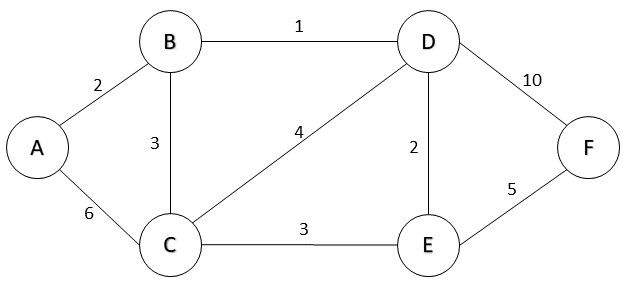
\includegraphics[width=100mm]{undirected_graph1.png}
	\caption{Ένα μη κατευθυνόμενο γράφημα 6 κορυφών και 9 ακμών με βάρη στις ακμές του}
	\label{fig:undirected_graph1}
\end{figure}

Ένα γράφημα λέγεται συνεκτικό αν για δύο οποιεσδήποτε κορυφές του υπάρχει μονοπάτι που τις συνδέει. Αν ένα γράφημα δεν είναι συνεκτικό τότε αποτελείται από επιμέρους συνεκτικά γραφήματα τα οποία λέγονται συνιστώσες. Είναι προφανές ότι ένα συνεκτικό γράφημα έχει μόνο μια συνιστώσα.

\subsection{Αναπαράσταση γραφημάτων}
Δύο διαδεδομένοι τρόποι αναπαράστασης γραφημάτων είναι οι πίνακες γειτνίασης (adjacency matrices) και οι λίστες γειτνίασης (adjacency lists).

Στους πίνακες γειτνίασης διατηρείται ένας δισδιάστατος πίνακας $n \times n$ όπου $n$ είναι το πλήθος των κορυφών του γραφήματος. Για κάθε ακμή του γραφήματος που συνενώνει την κορυφή $i$ με την κορυφή $j$ εισάγεται στη θέση $i,j$ του πίνακα το βάρος της ακμής αν το γράφημα είναι με βάρη ενώ αν δεν υπάρχουν βάρη τότε εισάγεται η τιμή 1. Όλα τα υπόλοιπα στοιχεία του πίνακα λαμβάνουν την τιμή 0. Για παράδειγμα η πληροφορία του γραφήματος για το σχήμα \ref{fig:undirected_graph1} διατηρείται όπως φαίνεται στον πίνακα \ref{tbl:adjacency_table}.

% Please add the following required packages to your document preamble:
% \usepackage[table,xcdraw]{xcolor}
% If you use beamer only pass "xcolor=table" option, i.e. \documentclass[xcolor=table]{beamer}
\begin{table}[ht]
	\centering
	\begin{tabular}{|
		>{\columncolor[HTML]{C0C0C0}}l |c|c|c|c|c|c|}
		\hline
		\cellcolor[HTML]{FFFFFF} & \cellcolor[HTML]{C0C0C0} A & \cellcolor[HTML]{C0C0C0} B & \cellcolor[HTML]{C0C0C0} C & \cellcolor[HTML]{C0C0C0}D & \cellcolor[HTML]{C0C0C0} E & \cellcolor[HTML]{C0C0C0} F \\ \hline
		A                        & 0                          & 2                          & 6                          & 0                         & 0                          & 0                          \\ \hline
		B                        & 2                          & 0                          & 3                          & 1                         & 0                          & 0                          \\ \hline
		C                        & 6                          & 3                          & 0                          & 4                         & 3                          & 0                          \\ \hline
		D                        & 0                          & 1                          & 4                          & 0                         & 2                          & 10                         \\ \hline
		E                        & 0                          & 0                          & 3                          & 2                         & 0                          & 5                          \\ \hline
		F                        & 0                          & 0                          & 0                          & 10                        & 5                          & 0                          \\ \hline
	\end{tabular}
	\caption{Πίνακας γειτνίασης για το σχήμα \ref{fig:undirected_graph1}}
    \label{tbl:adjacency_table}
\end{table}

Στις λίστες γειτνίασης διατηρούνται λίστες που περιέχουν για κάθε κορυφή όλη την πληροφορία των συνδέσεών της με τους γειτονικούς της κόμβους. Για παράδειγμα το γράφημα του σχήματος \ref{fig:undirected_graph1} μπορεί να αναπαρασταθεί με τις ακόλουθες 6 λίστες (μια ανά κορυφή). Κάθε στοιχείο της λίστας για την κορυφή $v$ είναι ένα ζεύγος τιμών $(w,u)$ και αναπαριστά μια ακμή από την κορυφή $v$ στην κορυφή $u$ με βάρος $w$, όπως φαίνεται στο πίνακα \ref{tbl:adjacency_list}.

\begin{table}[ht]
	\centering
	\begin{tabular}{|
		>{\columncolor[HTML]{C0C0C0}}l |c|}
		\hline
		A & (2,B), (6,C)                \\ \hline
		B & (2,A), (3,C), (1,D)         \\ \hline
		C & (6,A), (3,B), (4,D), (3,E)  \\ \hline
		D & (1,B), (4,C), (2,E), (10,F) \\ \hline
		E & (3,C), (2,D), (5,F)         \\ \hline
		F & (10,D), (5,E)               \\ \hline
	\end{tabular}
	\caption{Λίστα γειτνίασης για το σχήμα \ref{fig:undirected_graph1}}
	\label{tbl:adjacency_list}
\end{table}

Περισσότερα για τις αναπαραστάσεις γραφημάτων μπορούν να βρεθούν στις αναφορές \cite{g4g_graph_representations} και \cite{he_graph_representations}.

\subsection{Ανάγνωση δεδομένων γραφήματος από αρχείο}
Υπάρχουν πολλοί τρόποι με τους οποίους μπορούν να βρίσκονται καταγεγραμμένα τα δεδομένα ενός γραφήματος σε ένα αρχείο. Το αρχείο αυτό θα πρέπει να διαβαστεί έτσι ώστε να αναπαρασταθεί το γράφημα στη μνήμη του υπολογιστή. Στη συνέχεια παρουσιάζεται μια απλή μορφή αποτύπωσης κατευθυνόμενων με βάρη γραφημάτων χρησιμοποιώντας αρχεία απλού κειμένου. Σύμφωνα με αυτή τη μορφή για κάθε κορυφή του γραφήματος καταγράφεται σε ξεχωριστή γραμμή του αρχείου κειμένου το όνομά της ακολουθούμενο από ζεύγη τιμών, χωρισμένων με κόμματα, που αντιστοιχούν στις ακμές που ξεκινούν από τη συγκεκριμένη κορυφή. Στο κείμενο που ακολουθεί (graph1.txt) και το οποίο αφορά το γράφημα του σχήματος \ref{fig:undirected_graph1} η πρώτη γραμμή σημαίνει ότι η κορυφή Α συνδέεται με μια ακμή με βάρος 2 με την κορυφή B καθώς και με μια ακμή με βάρος 6 με την κορυφή C. Ανάλογα καταγράφεται η πληροφορία ακμών και για τις άλλες κορυφές.

\lstinputlisting[style=DOS]{lab08/graph1.txt}

Η ανάγνωση του αρχείου και η αναπαράσταση του γραφήματος ως λίστα γειτνίασης γίνεται με τη συνάρτηση read\_data που δίνεται στη συνέχεια όπου fn είναι το όνομα του αρχείου. Η συνάρτηση αυτή δημιουργεί ένα λεξικό (map) που αποτελείται από εγγραφές τύπου key-value. Σε κάθε εγγραφή το key είναι ένα λεκτικό με το όνομα μιας κορυφής ενώ το value είναι ένα διάνυσμα (vector) που περιέχει ζεύγη (pair<int,string>) στα οποία το πρώτο στοιχείο είναι ένας ακέραιος αριθμός που αναπαριστά το βάρος μιας ακμής ενώ το δεύτερο ένα λεκτικό με το όνομα της κορυφής στην οποία καταλήγει η ακμή από την κορυφή key. Ο κώδικας έχει ``σπάσει'' σε 3 αρχεία (graph.hpp, graph.cpp και graph\_ex1.cpp) έτσι ώστε να είναι ευκολότερη η επαναχρησιμοποίηση του. Η συνάρτηση print\_data εμφανίζει τα δεδομένα του γραφήματος.

\lstinputlisting[caption = header file με τις συναρτήσεις για ανάγνωση και εμφάνιση γραφημάτων (graph.hpp)]{lab08/graph.hpp}

\lstinputlisting[caption = source file με τις συναρτήσεις για ανάγνωση και εμφάνιση γραφημάτων (graph.cpp),multicols=2]{lab08/graph.cpp}

\lstinputlisting[caption = Ανάγνωση και εκτύπωση των δεδομένων του γραφήματος του σχήματος \ref{fig:undirected_graph1} (graph\_ex1.cpp)]{lab08/graph_ex1.cpp}

Η μεταγλώττιση και η εκτέλεση του κώδικα γίνεται με τις ακόλουθες εντολές:

\lstinputlisting[style=DOS]{lab08/compile_execute1.txt}

Η δε έξοδος που παράγεται είναι η ακόλουθη:

\lstinputlisting[style=DOS]{lab08/graph_ex1.out}

\subsection{Κατευθυνόμενα ακυκλικά γραφήματα}
Τα κατευθυνόμενα ακυκλικά γραφήματα (Directed Acyclic Graphs=DAGs) είναι γραφήματα για τα οποία δεν μπορεί να εντοπιστεί διαδρομή από μια κορυφή προς την ίδια. Στο σχήμα \ref{fig:dag1} παρουσιάζεται ένα γράφημα το οποίο δεν παρουσιάζει κύκλους. Αν για παράδειγμα υπήρχε μια ακόμα ακμή από την κορυφή E προς την κορυφή A τότε πλέον το γράφημα δεν θα ήταν DAG καθώς θα υπήρχε ο κύκλος A-C-E-A.

\begin{figure}[ht]
	\centering
	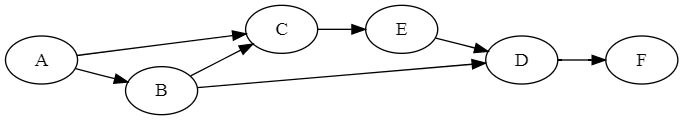
\includegraphics[width=120mm]{dag1.png}
	\caption{Ένα κατευθυνόμενο ακυκλικό γράφημα (DAG)}
	\label{fig:dag1}
\end{figure}

Τα DAGs χρησιμοποιούνται στη μοντελοποίηση πολλών καταστάσεων. Μπορούν για παράδειγμα να αναπαραστήσουν εργασίες που πρέπει να εκτελεστούν και για τις οποίες υπάρχουν εξαρτήσεις όπως για παράδειγμα ότι για να ξεκινήσει η εκτέλεση της εργασίας D θα πρέπει πρώτα να έχουν ολοκληρωθεί οι εργασίες B και E. 

\subsection{Σημαντικοί αλγόριθμοι γραφημάτων}
Υπάρχουν πολλοί αλγόριθμοι που εφαρμόζονται σε γραφήματα προκειμένου να επιλύσουν ενδιαφέροντα προβλήματα που ανακύπτουν σε πρακτικές εφαρμογές. Οι ακόλουθοι αλγόριθμοι είναι μερικοί από αυτούς:
\begin{itemize}[noitemsep]
	\item Αναζήτηση συντομότερων διαδρομών από μια κορυφή προς όλες τις άλλες κορυφές (Dijkstra). Ο αλγόριθμος αυτός θα αναλυθεί στη συνέχεια.
	\item Εύρεση μήκους συντομότερων διαδρομών για όλα τα ζεύγη κορυφών (Floyd Warshall) \cite{pa_floyd_warshall}.
	\item Αναζήτηση κατά βάθος (Depth First Search). Είναι αλγόριθμος διάσχισης γραφήματος ο οποίος ξεκινά από έναν κόμβο αφετηρία και επισκέπτεται όλους τους άλλους κόμβους που είναι προσβάσιμοι χρησιμοποιώντας της ακμές του γραφήματος. Λειτουργεί επεκτείνοντας μια διαδρομή όσο βρίσκει νέους κόμβους τους οποίους μπορεί να επισκεφθεί. Αν δεν βρίσκει νέους κόμβους οπισθοδρομεί και διερευνά άλλα τμήματα του γραφήματος.
	\item Αναζήτηση κατά πλάτος (Breadth First Search). Αλγόριθμος διάσχισης γραφήματος που ξεκινώντας από έναν κόμβο αφετηρία επισκέπτεται τους υπόλοιπους κόμβους σε αύξουσα σειρά βημάτων από την αφετηρία. Βήματα θεωρούνται οι μεταβάσεις από κορυφή σε κορυφή.
	\item Εντοπισμός ελάχιστου συνεκτικού (ή γεννητικού) δένδρου (Prim \cite{programiz_prim}, Kruskal \cite{programiz_kruskal}). Δεδομένου ενός γραφήματος, το πρόβλημα αφορά την εύρεση ενός δένδρου στο οποίο θα περιέχονται όλες οι κορυφές του γραφήματος ενώ οι ακμές του δένδρου θα είναι ένα υποσύνολο των ακμών του γραφήματος τέτοιο ώστε το άθροισμα των βαρών τους να είναι το ελάχιστο δυνατό.
	\item Τοπολογική ταξινόμηση (Topological Sort) \cite{g4g_topological_sort}. Ο αλγόριθμος τοπολογικής ταξινόμησης εφαρμόζεται σε DAGs και παράγει μια σειρά κορυφών του γραφήματος για την οποία ισχύει ότι για κάθε κατευθυνόμενη ακμή από την κορυφή $u$ στην κορυφή $v$ στη σειρά των κορυφών η κορυφή $u$ προηγείται της κορυφής $v$. Για παράδειγμα, για το DAG του σχήματος \ref{fig:dag1} αποτέλεσμα του αλγορίθμου είναι το A,B,C,E,D,F. Σε συνθετότερα γραφήματα μπορεί να υπάρχουν περισσότερες από μια τοπολογικές σειρές κορυφών για το γράφημα.
	\item Εντοπισμός κυκλωμάτων Euler (Eulerian circuit) \cite{dicretetext_euler_path}. Σε ένα γράφημα, διαδρομή Euler (Eulerian path) είναι μια διαδρομή που περνά από όλες τις ακμές του γραφήματος. Αν η διαδρομή αυτή ξεκινά και τερματίζει στην ίδια κορυφή τότε λέγεται κύκλωμα Euler. 
	\item Εντοπισμός ισχυρά συνδεδεμένων συνιστωσών (Strongly Connected Components) \cite{he_scc}. Ισχυρά συνδεδεμένες συνιστώσες υφίστανται μόνο σε κατευθυνόμενα γραφήματα. Ένα κατευθυνόμενο γράφημα είναι ισχυρά συνδεδεμένο όταν υπάρχει διαδρομή από κάθε κορυφή προς κάθε άλλη κορυφή. Ένα κατευθυνόμενο γράφημα μπορεί να σπάσει σε ισχυρά συνδεδεμένα υπογραφήματα. Τα υπογραφήματα αυτά αποτελούν τις ισχυρά συνδεδεμένες συνιστώσες του γραφήματος.
\end{itemize} 

 
\section{Αλγόριθμος του Dijkstra για εύρεση συντομότερων διαδρομών}
Ο αλγόριθμος δέχεται ως είσοδο ένα γράφημα $G=(V,E)$ και μια κορυφή του γραφήματος $s$ η οποία αποτελεί την αφετηρία. Υπολογίζει για όλες τις κορυφές $v \in V$ το μήκος του συντομότερου μονοπατιού από την κορυφή $s$ στην κορυφή $v$. Για να λειτουργήσει σωστά θα πρέπει κάθε ακμή να έχει μη αρνητικό βάρος. Αν το γράφημα περιέχει ακμές με αρνητικό βάρος τότε μπορεί να χρησιμοποιηθεί ο αλγόριθμος των Bellman-Ford \cite{brilliant_bellman_ford}.

\subsection{Περιγραφή του αλγορίθμου}
Ο αλγόριθμος εντοπίζει τις συντομότερες διαδρομές προς τις κορυφές του γραφήματος σε σειρά απόστασης από την κορυφή αφετηρία. Σε κάθε βήμα του αλγορίθμου η αφετηρία και οι ακμές προς τις κορυφές για τις οποίες έχει ήδη βρεθεί συντομότερο μονοπάτι σχηματίζουν το υποδένδρο $S$ του γραφήματος. Οι κορυφές που είναι προσπελάσιμες με 1 ακμή από το υποδένδρο $S$ είναι υποψήφιες να αποτελέσουν την επόμενη κορυφή που θα εισέλθει στο υποδένδρο. Επιλέγεται μεταξύ τους η κορυφή που βρίσκεται στη μικρότερη απόσταση από την αφετηρία. Για κάθε υποψήφια κορυφή $u$ υπολογίζεται το άθροισμα της απόστασής της από την πλησιέστερη κορυφή $v$ του δένδρου συν το μήκος της συντομότερης διαδρομής από την αφετηρία $s$ προς την κορυφή $v$. Στη συνέχεια επιλέγεται η κορυφή με το μικρότερο άθροισμα και προσαρτάται στο σύνολο των κορυφών που απαρτίζουν το υποδένδρο $S$. Για κάθε μία από τις υποψήφιες κορυφές που συνδέονται με μια ακμή με την κορυφή που επιλέχθηκε ενημερώνεται η απόστασή της από το υποδένδρο εφόσον προκύψει μικρότερη τιμή.

\paragraph{Ψευδοκώδικας}
Το σύνολο $S$ περιέχει τις κορυφές για τις οποίες έχει προσδιοριστεί η συντομότερη διαδρομή από την κορυφή $s$ ενώ το διάνυσμα $d$ περιέχει τις αποστάσεις από την κορυφή $s$ \\
1. Αρχικά $S={s}$, $d_s=0$ και για όλες τις κορυφές $i \neq s, d_i=\infty$ \\
2. Μέχρι να γίνει $S=V$ \\
3. Εντοπισμός του στοιχείου $v \notin S$ με τη μικρότερη τιμή $d_v$ και προσθήκη του στο $S$ \\
4. Για κάθε ακμή από την κορυφή $v$ στην κορυφή $u$ με βάρος $w$ ενημερώνεται η τιμή $d_u$ έτσι ώστε: \\
\centerline{$d_u=min(d_u, d_v+w)$}
5. Επιστροφή στο βήμα 2.

\paragraph{Εκτέλεση του αλγορίθμου}
Στη συνέχεια ακολουθεί παράδειγμα εκτέλεσης του αλγορίθμου για το γράφημα του σχήματος \ref{fig:undirected_graph1}.

\begin{table}[ht]
	\centering
	\label{tbl:dijkstra1}
	\begin{tabular}{|c|p{5cm}|}
		\hline
		$S=\{A\},d_A=0,d_B=2,d_C=6,d_D=\infty,d_E=\infty,d_F=\infty $   & Από το $S$ μπορούμε να φτάσουμε στις κορυφές B και C με μήκος διαδρομής 2 και 6 αντίστοιχα. Επιλέγεται η κορυφή B.                                                                                         \\ \hline
		$S=\{A,B\}, d_A=0, d_B=2, d_C=5, d_D=3, d_E=\infty, d_F=\infty$ & Από το $S$ μπορούμε να φτάσουμε στις κορυφές C και D με μήκος διαδρομής 5 και 3 αντίστοιχα. Επιλέγεται η κορυφή D.                                                                                         \\ \hline
		$S= \{A,B,D\},d_A=0,d_B=2,d_C=5,d_D=3,d_E=5,d_F=13$             & Από το $S$ μπορούμε να φτάσουμε στις κορυφές C, E και F με μήκος διαδρομής 5, 5 και 13 αντίστοιχα. Επιλέγεται (με τυχαίο τρόπο) ανάμεσα στις κορυφές C και E η κορυφή C. \\ \hline
		$S=\{A,B,D,C\},d_A=0,d_B=2,d_C=5,d_D=3,d_E=5,d_F=13$            & Από το $S$ μπορούμε να φτάσουμε στις κορυφές E και F με μήκος διαδρομής 5 και 13 αντίστοιχα. Επιλέγεται η κορυφή E.                                                                                        \\ \hline
		$S=\{A,B,D,C,E\},d_A=0,d_B=2,d_C=5,d_D=3,d_E=5,d_F=10$          & Η μοναδική κορυφή στην οποία μένει να φτάσουμε από το $S$ είναι η κορυφή F και το μήκος της συντομότερης διαδρομής από την A στην F είναι 10.                                        \\ \hline
		\multicolumn{2}{|c|}{$S=\{A,B,D,C,E,F\},d_A=0,d_B=2,d_C=5,d_D=3,d_E=5,d_F=10$ } \\ \hline
	\end{tabular}
	\caption{Αναλυτική εκτέλεση του αλγορίθμου}
\end{table}

\begin{table}[ht]
	\centering
	\label{tbl:dijkstra2}
	\begin{tabular}{|c|c|c|c|c|c|c|}
		\hline
		Σύνολο $S$  & A & B        & C        & D        & E        & F        \\ \hline
		$\{\}$            & 0 & $\infty$     & $\infty$ & $\infty$ & $\infty$ & $\infty$ \\ \hline
		$\{A\}$           & 0 & $2_A$        & $6_A$        & $\infty$ & $\infty$ & $\infty$ \\ \hline
		$\{A,B\}$         & 0 & $2_A$        & $5_B$        & $3_B$        & $\infty$ & $\infty$ \\ \hline
		$\{A,B,D\}$       & 0 & $2_A$        & $5_B$        & $3_B$        & $5_D$        & $13_D$       \\ \hline
		$\{A,B,D,C\}$     & 0 & $2_A$        & $5_B$        & $3_B$        & $5_D$        & $13_D$       \\ \hline
		$\{A,B,D,C,E\}$   & 0 & $2_A$        & $5_B$        & $3_B$        & $5_D$        & $10_E$       \\ \hline
		$\{A,B,D,C,E,F\}$ & 0 & $2_A$        & $5_B$        & $3_B$        & $5_D$        & $10_E$       \\ \hline
	\end{tabular}
	\caption{Συνοπτική εκτέλεση του αλγορίθμου}
\end{table}

Συνεπώς ισχύει ότι: 
\begin{itemize}[noitemsep]
	\item Για την κορυφή A η διαδρομή αποτελείται μόνο από τον κόμβο A και έχει μήκος 0.
	\item Για την κορυφή B η διαδρομή είναι η A-B με μήκος 2.
	\item Για την κορυφή C η διαδρομή είναι η A-B-C με μήκος 5.
	\item Για την κορυφή D η διαδρομή είναι η A-B-D με μήκος 3.
	\item Για την κορυφή E η διαδρομή είναι η A-B-D-E με μήκος 5.
	\item Για την κορυφή F η διαδρομή είναι η A-B-D-E-F με μήκος 10.
\end{itemize}

Στο σύνδεσμο της αναφοράς \cite{algorithm_visualization_dijkstra} μπορεί κανείς να παρακολουθήσει την εκτέλεση του αλγορίθμου για διάφορα γραφήματα.

\paragraph{Απόδοση του αλγορίθμου}

Η ταχύτητα εκτέλεσης του αλγορίθμου εξαρτάται από τις δομές δεδομένων που χρησιμοποιούνται για να αναπαρασταθεί το γράφημα. Γενικά, πρόκειται για έναν εξαιρετικά γρήγορο αλγόριθμο με πολυπλοκότητα χειρότερης περίπτωσης $O(|E| log |V|)$, όπου $|E|$ είναι ο αριθμός των ακμών και $|V|$ ο αριθμός των κορυφών του γραφήματος.

\subsection{Κωδικοποίηση του αλγορίθμου}
\lstinputlisting[caption = header file για τον αλγόριθμο του Dijkstra (dijkstra.hpp),multicols=2]{lab08/dijkstra.hpp}

\lstinputlisting[caption = source file για τον αλγόριθμο του Dijkstra (dijkstra.cpp),multicols=2]{lab08/dijkstra.cpp}

\lstinputlisting[caption = source file προγράμματος που καλεί τον αλγόριθμο του Dijkstra (dijkstra\_ex1.cpp)]{lab08/dijkstra_ex1.cpp}

Η μεταγλώττιση και η εκτέλεση του κώδικα γίνεται με τις ακόλουθες εντολές:

\lstinputlisting[style=DOS]{lab08/compile_execute2.txt}

Η δε έξοδος που παράγεται είναι η ακόλουθη:

\lstinputlisting[style=DOS]{lab08/dijkstra_ex1.out}


\section{Παραδείγματα}

\subsection{Παράδειγμα 1}
Για το σχήμα \ref{fig:undirected_graph2} και με αφετηρία την κορυφή A συμπληρώστε τον πίνακα εκτέλεσης του αλγορίθμου για την εύρεση των συντομότερων διαδρομών του Dijkstra και καταγράψτε τις διαδρομές που εντοπίζονται από την αφετηρία προς όλες τις άλλες κορυφές.

\begin{figure}[ht!]
	\centering
	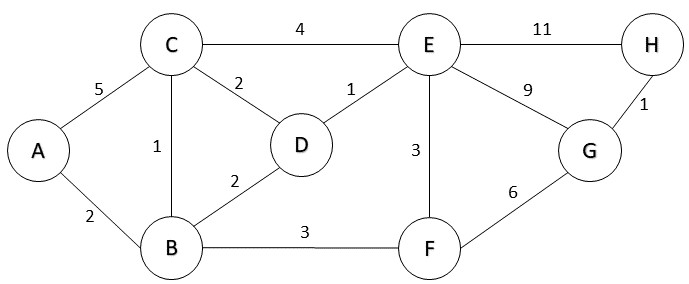
\includegraphics[width=120mm]{undirected_graph2.png}
	\caption{Ένα μη κατευθυνόμενο γράφημα 8 κορυφών με βάρη στις ακμές του}
	\label{fig:undirected_graph2}
\end{figure}

Ο ακόλουθος πίνακας δείχνει την εκτέλεση του αλγορίθμου
\begin{table}[ht!]
	\centering
	\label{tbl:dijkstra3}
	\begin{tabular}{|c|c|c|c|c|c|c|c|c|}
		\hline
		Σύνολο $S$            & A & B        & C        & D        & E        & F        & G        & H         \\ \hline
		$\{\}$                & 0 & $\infty$ & $\infty$ & $\infty$ & $\infty$ & $\infty$ & $\infty$ & $\infty$  \\ \hline
		$\{A\}$               & 0 & $2_A$    & $5_A$    & $\infty$ & $\infty$ & $\infty$ & $\infty$ & $\infty$  \\ \hline
		$\{A,B\}$             & 0 & $2_A$    & $3_B$    & $\infty$ & $\infty$ & $5_B$    & $\infty$ & $\infty$  \\ \hline
		$\{A,B,C\}$           & 0 & $2_A$    & $3_B$    & $4_B$    & $7_C$    & $5_B$    & $\infty$ & $\infty$  \\ \hline
		$\{A,B,C,D\}$         & 0 & $2_A$    & $3_B$    & $4_B$    & $5_D$    & $5_B$    & $\infty$ & $\infty$  \\ \hline
		$\{A,B,C,D,E\}$       & 0 & $2_A$    & $3_B$    & $4_B$    & $5_D$    & $5_B$    & $14_E$   & $16_E$    \\ \hline			
		$\{A,B,C,D,E,F\}$     & 0 & $2_A$    & $3_B$    & $4_B$    & $5_D$    & $5_B$    & $11_F$   & $16_E$    \\ \hline			
		$\{A,B,C,D,E,F,G\}$    & 0 & $2_A$    & $3_B$    & $4_B$    & $5_D$    & $5_B$    & $11_F$   & $12_E$    \\ \hline			
		$\{A,B,C,D,E,F,G,H\}$ & 0 & $2_A$    & $3_B$    & $4_B$    & $5_D$    & $5_B$    & $11_F$   & $12_E$    \\ \hline
	\end{tabular}
	\caption{Συνοπτική εκτέλεση του αλγορίθμου}
\end{table}


Οι συντομότερες διαδρομές είναι:
\begin{itemize}[noitemsep]
\item Για την κορυφή A η διαδρομή είναι η A με μήκος 0
\item Για την κορυφή B η διαδρομή είναι η A-B με μήκος 2
\item Για την κορυφή C η διαδρομή είναι η A-B-C με μήκος 3
\item Για την κορυφή D η διαδρομή είναι η A-B-D με μήκος 4
\item Για την κορυφή E η διαδρομή είναι η A-B-D-E με μήκος 5
\item Για την κορυφή F η διαδρομή είναι η A-B-F με μήκος 5
\item Για την κορυφή G η διαδρομή είναι η A-B-F-G με μήκος 11
\item Για την κορυφή H η διαδρομή είναι η A-B-F-G-H με μήκος 12
\end{itemize}

\subsection{Παράδειγμα 2}
Γράψτε πρόγραμμα που να διαβάζει ένα γράφημα και να εμφανίζει για κάθε κορυφή το βαθμό της, δηλαδή το πλήθος των κορυφών με τις οποίες συνδέεται απευθείας καθώς και το μέσο όρο βαρών για αυτές τις ακμές. Επιπλέον για κάθε κορυφή να εμφανίζει τις υπόλοιπες κορυφές οι οποίες μπορούν να προσεγγιστούν με διαδρομές μήκους 1,2,3 κοκ.

\lstinputlisting[caption = (lab08\_ex2.cpp),multicols=2]{lab08/lab08_ex2.cpp}

Η μεταγλώττιση και η εκτέλεση του κώδικα γίνεται με τις ακόλουθες εντολές:

\lstinputlisting[style=DOS]{lab08/compile_execute3.txt}

Η δε έξοδος που παράγεται είναι η ακόλουθη:

\lstinputlisting[style=DOS]{lab08/lab08_ex2.out}

\section{Ασκήσεις}
\begin{enumerate}[nolistsep]
	\item Υλοποιήστε τον αλγόριθμο των Bellman-Ford \cite{brilliant_bellman_ford} για την εύρεση της συντομότερης διαδρομής από μια κορυφή προς όλες τις άλλες κορυφές.
	\item Υλοποιήστε έναν αλγόριθμο τοπολογικής ταξινόμησης για DAGs \cite{g4g_topological_sort}.
\end{enumerate}

\begin{thebibliography}{9}
\bibitem{g4g_graph_representations}
Geeks for Geeks, graphs and its representations, \href{https://www.geeksforgeeks.org/graph-and-its-representations/}{https://www.geeksforgeeks.org/graph-and-its-representations/}

\bibitem{he_graph_representations}
HackerEarth, graph representation, \href{https://www.hackerearth.com/practice/algorithms/graphs/graph-representation/tutorial/}{https://www.hackerearth.com/practice/algorithms/graphs/graph-representation/tutorial/}

\bibitem{pa_floyd_warshall}
Programming-Algorithms.net, Floyd-Warshall algorithm, \href{http://www.programming-algorithms.net/article/45708/Floyd-Warshall-algorithm}{http://www.programming-algorithms.net/article/45708/Floyd-Warshall-algorithm}

\bibitem{programiz_prim}
PROGRAMIZ, Prim's algorithm, \href{https://www.programiz.com/dsa/prim-algorithm}{https://www.programiz.com/dsa/prim-algorithm}

\bibitem{programiz_kruskal}
PROGRAMIZ, Kruskal's algorithm, \href{https://www.programiz.com/dsa/kruskal-algorithm}{https://www.programiz.com/dsa/kruskal-algorithm}

\bibitem{g4g_topological_sort}
Geeks for Geeks, topological sorting, \href{https://www.geeksforgeeks.org/topological-sorting/}{https://www.geeksforgeeks.org/topological-sorting/}

\bibitem{dicretetext_euler_path}
Discrete Mathematics: An open introduction by Oscar Levin, Euler Paths and Circuits, \href{http://discretetext.oscarlevin.com/dmoi/sec_paths.html}{http://discretetext.oscarlevin.com/dmoi/sec\_paths.html}

\bibitem{he_scc}
HackerEarth, Strongly Connected Components, \href{https://www.hackerearth.com/practice/algorithms/graphs/strongly-connected-components/tutorial/}{https://www.hackerearth.com/practice/algorithms/graphs/strongly-connected-components/tutorial/}

\bibitem{brilliant_bellman_ford}
Brilliant.org, Bellman-Ford Algorithm, \href{https://brilliant.org/wiki/bellman-ford-algorithm/}{https://brilliant.org/wiki/bellman-ford-algorithm/}

\bibitem{algorithm_visualization_dijkstra}
Algorithm visualization, Dijkstra's shortest path, \href{https://www.cs.usfca.edu/~galles/visualization/Dijkstra.html}{https://www.cs.usfca.edu/~galles/visualization/Dijkstra.html}

\end{thebibliography}


% Εργαστήριο 9
\chapter{Δένδρα}
\section{Εισαγωγή}
Τα δένδρα όπως και τα γραφήματα είναι μη γραμμικές δομές δεδομένων που αποτελούν συλλογές κόμβων. Τα δένδρα επιτρέπουν ιεραρχική οργάνωση των δεδομένων όπως φαίνεται στο Σχήμα \ref{fig:binary_tree}. Αυτό το στοιχείο τους επιτρέπει να έχουν καλύτερες επιδόσεις προσπέλασης των επιμέρους στοιχείων σε σχέση με τις γραμμικές λίστες. Με κατάλληλη διευθέτηση των στοιχείων ενός δένδρου καθώς και με εφαρμογή προχωρημένων μηχανισμών εισαγωγής και διαγραφής στοιχείων ο χρόνος εκτέλεσης των περισσότερων λειτουργιών σε ένα δένδρο (ισοζυγισμένο δυαδικό δένδρο αναζήτησης) γίνεται $O(\log n)$. Στην STL τα δένδρα χρησιμοποιούνται στην υλοποίηση των containers std::map και std::set.

\begin{figure}[htbp]
  \centering
  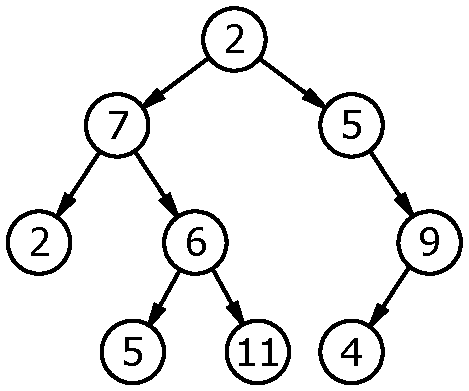
\includegraphics[width=80mm]{Binary_tree.pdf}
  \caption{Ένα απλό δένδρο \cite{wikipedia_binary_tree}}
  \label{fig:binary_tree}
\end{figure}

\section{Δένδρα}

Ένα δένδρο (tree) αποτελείται από κόμβους (nodes) που συνδέονται μεταξύ τους με κατευθυνόμενες ακμές (edges). Ο πρώτος (υψηλότερος) κόμβος του δένδρου ονομάζεται ρίζα (root) ενώ οι κόμβοι που βρίσκονται στα άκρα του δένδρου λέγονται φύλλα (leaves). Οι κόμβοι με τους οποίους συνδέεται απευθείας ένας κόμβος ονομάζονται παιδιά (children) του κόμβου. Αντίστοιχα, ένας κόμβος που έχει παιδιά ονομάζεται γονέας (parent) των αντίστοιχων παιδιών-κόμβων. Απόγονοι (descendants) ενός κόμβου είναι οι κόμβοι για τους οποίους υπάρχει διαδρομή-μονοπάτι (path) πραγματοποιώντας διαδοχικές μεταβάσεις από γονείς σε παιδιά. Αντίστοιχα ορίζεται και η έννοια των προγόνων (ancestors) ενός κόμβου με τη ρίζα να είναι ο μοναδικός κόμβος που δεν έχει προγόνους. 

Τα δένδρα είναι αναδρομικές δομές από τη φύση τους. Κάθε κόμβος ενός δένδρου ορίζει έναν αριθμό από μικρότερα δένδρα, ένα για κάθε παιδί του. Σε ένα δένδρο με $N$ κόμβους υπάρχουν πάντα $N-1$ ακμές καθώς όλοι οι κόμβοι εκτός από τον κόμβο ρίζα έχουν μια ακμή η οποία τους συνδέει με τον γονέα τους.

Το μήκος ενός μονοπατιού ανάμεσα σε δύο κόμβους είναι ίσο με το πλήθος των ακμών του μονοπατιού. Εφόσον υπάρχει μονοπάτι μέσω του οποίου συνδέονται δύο κόμβοι το μονοπάτι αυτό είναι μοναδικό. Για κάθε κόμβο ορίζεται ως \textbf{βάθος του κόμβου} (depth) το μήκος του μονοπατιού από τη ρίζα του δένδρου μέχρι τον ίδιο τον κόμβο. Αντίστοιχα, \textbf{ύψος ενός κόμβου} (height) είναι το μήκος του μακρύτερου μονοπατιού από τον κόμβο προς ένα από τα φύλλα του δένδρου για τα οποία υφίσταται μονοπάτι με αφετηρία τον κόμβο.


\section{Δυαδικά δένδρα}

Δυαδικό δένδρο είναι ένα δένδρο για το οποίο ισχύει ότι κάθε κόμβος έχει το πολύ δύο παιδιά \cite{parlante_binary_tree}. Ένα δένδρο μπορεί να διανυθεί με διαφορετικούς τρόπους. Ορισμένοι βασικοί τρόποι διάσχισης (traversal) του δένδρου παρουσιάζονται στη συνέχεια \cite{g4g_traversals}.

\subsection{Αναζήτηση κατά βάθος}

Η αναζήτηση κατά βάθος (DFS = Depth First Search) διανύει το δένδρο αναζήτησης εξαντλώντας μονοπάτια από τη ρίζα προς τα φύλλα του δένδρου. Ένας τρόπος για να επιτευχθεί αυτό είναι η χρήση αναδρομής. 

\subsubsection{Προ-διατακτική αναζήτηση κατά βάθος}

Στη διάσχιση του δένδρου προ-διατακτικά (pre-order) πρώτα πραγματοποιείται η επίσκεψη στη ρίζα και μετά καλείται αναδρομικά η ίδια συνάρτηση πρώτα για το αριστερό υποδένδρο και μετά για το δεξιό υποδένδρο. 
Συνηθισμένες χρήσεις της pre-order διάσχισης είναι η δημιουργία αντιγράφων ενός δένδρου καθώς και η λήψη της prefix μορφής ενός expression tree \cite{wikipedia_polish_notation}.

\subsubsection{Ένδο-διατακτική αναζήτηση κατά βάθος}

Στη διάσχιση του δένδρου ένδο-διατακτικά (in-order) καλείται αναδρομικά η συνάρτηση για το αριστερό υποδένδρο, μετά πραγματοποιείται επίσκεψη στη ρίζα και μετά καλείται αναδρομικά η συνάρτηση για το δεξιό υποδένδρο.
Εφόσον το δένδρο είναι δυαδικό δένδρο αναζήτησης, η in-order διάσχιση επιστρέφει τους κόμβους σε μη φθίνουσα σειρά. Σχετικά με το τι είναι τα δυαδικά δένδρα αναζήτησης δείτε την παράγραφο~\ref{bst}).

\subsubsection{Μέτα-διατακτική αναζήτηση κατά βάθος}

Στη διάσχιση του δένδρου μέτα-διατακτικά (post-order) πρώτα καλείται αναδρομικά η  συνάρτηση για το αριστερό υποδένδρο, μετά καλείται αναδρομικά για το δεξιό υποδένδρο και τέλος πραγματοποιείται η επίσκεψη στη ρίζα. 
Συνηθισμένες χρήσεις της post-order διάσχισης είναι η διαγραφή ενός δένδρου καθώς και η λήψη της postfix μορφής ενός expression tree \cite{wikipedia_reverse_polish_notation}.

\subsection{Αναζήτηση κατά πλάτος}

Στην αναζήτηση κατά πλάτος (BFS=Breadth First Search) οι κόμβοι του δένδρου διανύονται κατά επίπεδα ξεκινώντας από τη ρίζα και μεταβαίνοντας από πάνω προς τα κάτω. Σε κάθε επίπεδο η προσπέλαση στους κόμβους γίνεται από αριστερά προς τα δεξιά. Για να επιτευχθεί αυτό το είδος διάσχισης του δένδρου χρησιμοποιείται μια ουρά (queue) στην οποία μόλις εξετάζεται ένα στοιχείο προστίθενται στο πίσω άκρο της ουράς τα παιδιά του.

\lstinputlisting[caption = header file για το δυαδικό δένδρο (binary\_tree.hpp)]{lab09/binary_tree.hpp}

\lstinputlisting[caption = source file για το δυαδικό δένδρο αναζήτησης (binary\_tree.cpp),multicols=2]{lab09/binary_tree.cpp}

Ο ακόλουθος κώδικας δημιουργεί το δυαδικό δένδρο του Σχήματος~\ref{fig:binary_tree1}.

\begin{figure}[htbp]
  \centering
  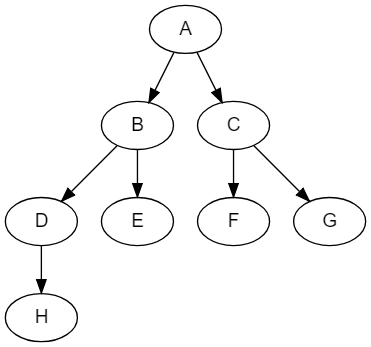
\includegraphics[width=80mm]{binary_tree1.png}
  \caption{Δυαδικό δένδρο με λεκτικά ως τιμές κλειδιών στους κόμβους}
  \label{fig:binary_tree1}
\end{figure}

\lstinputlisting[caption = Δοκιμή των συναρτήσεων του δυαδικού δένδρου (binary\_tree\_ex1.cpp)]{lab09/binary_tree_ex1.cpp}

Η μεταγλώττιση και η εκτέλεση του κώδικα γίνεται με τις ακόλουθες εντολές:

\lstinputlisting[style=DOS]{lab09/compile_execute1.txt}

Η δε έξοδος που παράγεται και για τους 4 τρόπους διάσχισης του δένδρου είναι η ακόλουθη:

\lstinputlisting[style=DOS]{lab09/binary_tree_ex1.out}


\section{Δυαδικά δένδρα αναζήτησης}
\label{bst}
Σε ένα δυαδικό δένδρο αναζήτησης θα πρέπει να ισχύει ότι για κάθε κόμβο όλες οι τιμές κλειδιών στο δένδρο αριστερά του κόμβου θα πρέπει να είναι μικρότερες από την τιμή κλειδιού του κόμβου. Αντίστοιχα, όλες οι τιμές κλειδιών στο δένδρο δεξιά του κάθε κόμβου θα πρέπει να είναι μεγαλύτερες από την τιμή κλειδιού του κόμβου.

\subsection{Υλοποίηση δυαδικού δένδρου αναζήτησης}

Ιδιαίτερη προσοχή θα πρέπει να δοθεί στην υλοποίηση της διαγραφής ενός κόμβου από το δένδρο έτσι ώστε το δένδρο και μετά τη διαγραφή να εξακολουθεί να είναι δυαδικό δένδρο αναζήτησης \cite{jumping_into_cpp}. 

\begin{figure}[!tbp]
  \centering
  \begin{minipage}[b]{0.4\textwidth}
    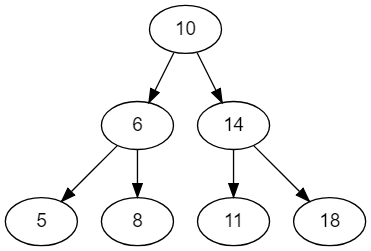
\includegraphics[width=\textwidth]{bst1.png}
    \label{fig:bst1}
    \caption{Δυαδικό δένδρο αναζήτησης}
  \end{minipage}
  \hfill
  \begin{minipage}[b]{0.4\textwidth}
    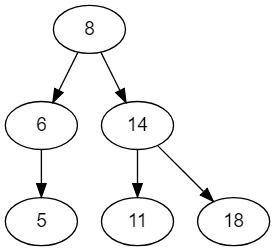
\includegraphics[width=\textwidth]{bst2.png}
    \label{fig:bst2}
    \caption{Το δυαδικό δένδρο αναζήτησης μετά τη διαγραφή της ρίζας}
  \end{minipage}
\end{figure}

\lstinputlisting[caption = header file για το δυαδικό δένδρο αναζήτησης (bst.hpp)]{lab09/bst.hpp}

\lstinputlisting[caption = source file για το δυαδικό δένδρο αναζήτησης (bst.cpp),multicols=2]{lab09/bst.cpp}

\lstinputlisting[caption = Δοκιμή των συναρτήσεων του δυαδικού δένδρου αναζήτησης (bst\_ex1.cpp),multicols=2]{lab09/bst_ex1.cpp}

Η μεταγλώττιση και η εκτέλεση του κώδικα γίνεται με τις ακόλουθες εντολές:

\lstinputlisting[style=DOS]{lab09/compile_execute2.txt}

Η δε έξοδος που παράγεται είναι η ακόλουθη:

\lstinputlisting[style=DOS]{lab09/bst_ex1.out}

Για να πραγματοποιηθεί η διαγραφή του κόμβου 10, εντοπίζεται ο κόμβος με τη μεγαλύτερη τιμή στο αριστερό υποδένδρο του κόμβου 10, που είναι ο 8 και ο κόμβος αυτός αφαιρείται από το δένδρο αντικαθιστώντας τον κόμβο 10.

\section{Ισοζυγισμένα δυαδικά δένδρα αναζήτησης}
\label{bbst}

Οι καλές επιδόσεις ενός δυαδικού δένδρου αναζήτησης χάνονται όταν το δένδρο δεν είναι ισοζυγισμένο (balanced), δηλαδή όταν υπάρχουν μονοπάτια από τη ρίζα προς τα φύλλα με μεγάλα βάθη ενώ άλλα μονοπάτια έχουν μικρά βάθη. Υπάρχουν διάφορες μορφές ισοζυγισμένων δένδρων με πλέον δημοφιλή τα κόκκινα-μαύρα δένδρα (red black trees) και τα AVL (Adelson, Velskii και Landis) δένδρα. Σε αυτά τα δένδρα πραγματοποιούνται ειδικές λειτουργίες (περιστροφές) έτσι ώστε κατά την εισαγωγή νέων τιμών στο δένδρο και τη διαγραφή τιμών από το δένδρο, τα βάθη των φύλλων του δένδρου εγγυημένα να διατηρούνται σε κοντινές τιμές μεταξύ τους. Ισχύει ότι τα AVL δένδρα είναι καλύτερα ισοζυγισμένα από τα κόκκινα-μαύρα δένδρα αλλά έχουν το μειονέκτημα της υψηλότερης υπολογιστικής επιβάρυνσης κατά την εισαγωγή και τη διαγραφή κόμβων.

\section{Παραδείγματα}

\subsection{Παράδειγμα 1}

Δεδομένου ενός δυαδικού δένδρου ζητείται η εκτύπωση όλων των διαδρομών από τη ρίζα του δένδρου μέχρι κάθε φύλλο. Για παράδειγμα, για το δένδρο του Σχήματος~\ref{fig:binary_tree1} το πρόγραμμα θα πρέπει να επιστρέψει ABDH, ABE, ACF και ACG.

\lstinputlisting[caption = Λύση παραδείγματος 1 (lab09\_ex1.cpp),multicols=2]{lab09/lab09_ex1.cpp}

Η μεταγλώττιση και η εκτέλεση του κώδικα γίνεται με τις ακόλουθες εντολές:

\lstinputlisting[style=DOS]{lab09/compile_execute3.txt}

Η έξοδος που παράγεται είναι η ακόλουθη:

\lstinputlisting[style=DOS]{lab09/lab09_ex1.out}


\subsection{Παράδειγμα 2}

Δεδομένου ενός δυαδικού δένδρου ζητείται να πραγματοποιείται έλεγχος σχετικά με το εάν το δένδρο είναι δυαδικό δένδρο αναζήτησης ή όχι. 

\lstinputlisting[caption = Λύση παραδείγματος 2 (lab09\_ex2.cpp),multicols=2]{lab09/lab09_ex2.cpp}

Η μεταγλώττιση και η εκτέλεση του κώδικα γίνεται με τις ακόλουθες εντολές:

\lstinputlisting[style=DOS]{lab09/compile_execute4.txt}

Η έξοδος που παράγεται είναι η ακόλουθη:

\lstinputlisting[style=DOS]{lab09/lab09_ex2.out}

\section{Ασκήσεις}

\begin{enumerate}[nolistsep]
\item Να γράψετε πρόγραμμα που να εμφανίζει τους κόμβους ενός δυαδικού δένδρου κατά επίπεδα από κάτω προς τα πάνω και από αριστερά προς τα δεξιά. Δηλαδή στο δένδρο του Σχήματος \ref{fig:binary_tree1} θα πρέπει οι κόμβοι να εμφανιστούν ως D, E, F, G, B, C, A.
\item Να γράψετε πρόγραμμα που να δημιουργεί από έναν ταξινομημένο πίνακα ακεραίων ένα δυαδικό δένδρο αναζήτησης. Να χρησιμοποιηθεί ο ακόλουθος αλγόριθμος:
	\begin{enumerate}[nolistsep]
	\item Εύρεση του μεσαίου στοιχείου του πίνακα και ορισμός του ως ρίζα του δένδρου
	\item Αναδρομική εκτέλεση για το αριστερό και το δεξιό μισό
		\begin{enumerate}[nolistsep]
		\item Εύρεση του μεσαίου στοιχείου του αριστερού μέρους και ορισμός του ως 		αριστερό παιδί της ρίζας του βήματος α'
		\item Εύρεση του μεσαίου στοιχείου του δεξιού μέρους και ορισμός του ως δεξί παιδί της ρίζας του βήματος α'
		\end{enumerate}
	\end{enumerate}
\end{enumerate}

\begin{thebibliography}{9}
\bibitem{wikipedia_binary_tree}
Wikipedia, Tree (data structure), \href{https://en.wikipedia.org/wiki/Tree_(data_structure)}{https://en.wikipedia.org/wiki/Tree\_(data\_structure)}

\bibitem{parlante_binary_tree}
Binary Trees by Nick Parlante, \href{http://cslibrary.stanford.edu/110/BinaryTrees.html}{http://cslibrary.stanford.edu/110/BinaryTrees.html}

\bibitem{wikipedia_polish_notation}
Wikipedia, Polish Notation, \href{https://en.wikipedia.org/wiki/Polish_notation}{https://en.wikipedia.org/wiki/Polish\_notation}

\bibitem{wikipedia_reverse_polish_notation}
Wikipedia, Reverse Polish Notation, \href{https://en.wikipedia.org/wiki/Reverse_Polish_notation}{https://en.wikipedia.org/wiki/Reverse\_Polish\_notation}

\bibitem{g4g_traversals}
Tree Traversals (Inorder, Preorder and Postorder), \href{https://www.geeksforgeeks.org/tree-traversals-inorder-preorder-and-postorder/}{https://www.geeksforgeeks.org/tree-traversals-inorder-preorder-and-postorder/}

\bibitem{jumping_into_cpp}
Alex Allain, Jumping into C++, cprogramming.com, Chapter 17 - Binary Trees, 2013

\end{thebibliography}



% Εργαστήριο 10
%\chapter{Δυναμικός προγραμματισμός}

\appendix
\chapter{Εγκατάσταση περιβάλλοντος ανάπτυξης προγραμμάτων C++}
\section*{Περιβάλλοντα ανάπτυξης εφαρμογών σε C++}
Υπάρχουν πολλοί τρόποι με τους οποίους μπορεί κανείς να αναπτύξει εφαρμογές σε C++. Κατ' ελάχιστο θα πρέπει να έχει πρόσβαση σε έναν compiler της C++ και σε έναν επεξεργαστή κειμένου. Διαδεδομένοι compilers της C++ είναι ο GNU compiler collection που περιέχει τον compiler της C (gcc) και τον compiler της C++ (g++), o clang, o Microsoft Visual C++ compiler, o C++ compiler της Intel (icc), o C++ compiler της Apple και άλλοι. Ομοίως, υπάρχουν πολλοί επεξεργαστές κειμένου που διευκολύνουν τη συγγραφή κώδικα όπως ο Visual Studio Code της Microsoft, ο SublimeText, o Atom και άλλοι.

Εναλλακτικά, μπορούν να χρησιμοποιηθούν τα γνωστά ως ολοκληρωμένα συστήματα ανάπτυξης εφαρμογών (IDEs=Integrated Development Environments). Ένα IDE διευκολύνει τη δημιουργία έργων (projects), ενσωματώνει πολλά εργαλεία (αποσφαλμάτωσης, εκτίμησης απόδοσης κώδικα, ελέγχου κώδικα κ.α.) και επιτρέπει τη διαχείριση των πόρων της εφαρμογής μέσα από ένα γνώριμο περιβάλλον. Διαδεδομένα IDEs είναι τα:
\begin{itemize}
\item Microsoft Visual Studio
\item JetBrains CLion
\item Xcode (για ανάπτυξη εφαρμογών σε υπολογιστές της Apple)
\item Netbeans for C++
\item Eclipse CDT
\item Code::Blocks
\item CodeLite
\item Geany 
\item Dev-C++
\end{itemize}  

\subsection*{Visual Studio Code και g++}
Ένας εύχρηστος τρόπος ανάπτυξης εφαρμογών σε C++ είναι χρησιμοποιώντας τον επεξεργαστή κειμένου της Microsoft, Visual Studio Code και το μεταγλωττιστή g++. Και τα δύο λογισμικά είναι ελεύθερα διαθέσιμα και μπορούν να εγκατασταθούν και στα τρία πλέον διαδεδομένα λειτουργικά συστήματα (Windows, Linux και macOS).   

\subsubsection*{Εγκατάσταση σε Windows}
Η εγκατάσταση του g++ στα Windows μπορεί να γίνει από το \href{https://nuwen.net/mingw.html}{https://nuwen.net/mingw.html} (MinGW Distro - nuwen.net) ακολουθώντας τις αναγραφόμενες οδηγίες. Η εγκατάσταση του Microsoft Visual Studio Code γίνεται πολύ απλά κατεβάζοντας και εκτελώντας το αντίστοιχο εκτελέσιμο από τη σελίδα του Visual Studio Code \href{https://code.visualstudio.com/}{https://code.visualstudio.com/}. Στη συνέχεια, μέσα από το Visual Studio Code πραγματοποιείται εγκατάσταση της επέκτασης (extention) C/C++, ms-vscode.cpptools.

\subsubsection*{Αποσφαλμάτωση μέσα από το Visual Studio Code χρησιμοποιώντας το gdb}
Έχοντας προηγηθεί η εγκατάσταση που περιγράφηκε στην προηγούμενη παράγραφο, το Visual Studio Code μπορεί πλέον να χρησιμοποιηθεί για αποσφαλμάτωση κώδικα. Για να συμβεί αυτό θα πρέπει στον ίδιο φάκελο με τον κώδικα να δημιουργηθούν τρία αρχεία, το c\_cpp\_properties.json, το tasks.json, και το launch.json. Στη συνέχεια περιγράφονται τα βήματα που απαιτούνται για να πραγματοποιηθεί αποσφαλμάτωση στο ακόλουθο πρόγραμμα. Αναλυτικότερες οδηγίες μπορούν να βρεθούν στο \href{https://code.visualstudio.com/docs/languages/cpp}{https://code.visualstudio.com/docs/languages/cpp}. 

\lstinputlisting[label=lst:bug1.cpp, caption=Κώδικας με σφάλμα (bug1.cpp)]{appendix_gdb/bug1.cpp}

Μεταγλωττίζοντας και εκτελώντας τον κώδικα διαπιστώνουμε ότι το αποτέλεσμα δεν είναι το αναμενόμενο καθώς θα έπρεπε να εμφανίζεται η μεγαλύτερη από τις τιμές του πίνακα (δηλαδή η τιμή 96) και όμως εμφανίζεται η τιμή 11. Τα βήματα που θα ακολουθηθούν έτσι ώστε να επιτευχθεί αποσφαλμάτωση του κώδικα εκτελώντας τις εντολές του μια προς μια είναι τα ακόλουθα.

\begin{enumerate}
\item Επιλέγοντας το μενού View \textrightarrow Command Palette \textrightarrow C/Cpp Edit configurations..., δημιουργείται το αρχείο c\_cpp\_properties.json στο οποίο θα πρέπει να τροποποιηθεί η ιδιότητα compilerPath έτσι ώστε να δείχνει τη θέση στην οποία βρίσκεται το εκτελέσιμο του compiler g++.

\begin{lstlisting}[style=DOS,caption=c\_cpp\_properties.json]
{
    "configurations": [
        {
            "name": "g++",
            "includePath": [
                "${workspaceFolder}/**"
            ],
            "defines": [
                "_DEBUG",
                "UNICODE",
                "_UNICODE"
            ],
            "compilerPath": "C:\\mingw\\bin\\g++.exe",
            "cStandard": "c11",
            "cppStandard": "c++17",
            "intelliSenseMode": "clang-x64"
        }
    ],
    "version": 4
}
\end{lstlisting}

\item Επιλέγοντας το μενού View \textrightarrow Command Palette \textrightarrow Tasks:Configure Tasks \textrightarrow Create tasks.json from template \textrightarrow msbuild, δημιουργείται το αρχείο tasks.json το οποίο θα πρέπει να τροποποιηθεί έτσι ώστε να έχει την ακόλουθη μορφή.

\begin{lstlisting}[style=DOS,caption=tasks.json]
{
    "version": "2.0.0",
    "tasks": [
        {
            "label": "build",
            "type": "shell",
            "command": "g++",
            "args": [
                "-g",
                "bug1.cpp"
            ],
            "group": {
                "kind": "build",
                "isDefault": true
            }
        }
    ]
}
\end{lstlisting}

Εφόσον έχει δημιουργηθεί το αρχείο tasks.json ο κώδικας μπορεί να μεταγλωττιστεί με το  μενού View \textrightarrow Command Palette \textrightarrow Tasks:Run Build Task, οπότε δημιουργείται το εκτελέσιμο a.exe.

\item Επιλέγοντας την προβολή Debug στο Visual Studio Code και στη συνέχεια από το μενού Debug \textrightarrow Add configuration..., δημιουργείται το αρχείο launch.json στο οποίο θα πρέπει να τροποποιηθούν οι ιδιότητες program και miDebuggerPath έτσι ώστε να δείχνουν στα κατάλληλα αρχεία όπως παρακάτω.  

\begin{lstlisting}[style=DOS,caption=launch.json]
{

    "version": "0.2.0",
    "configurations": [
        {
            "name": "(gdb) Launch",
            "type": "cppdbg",
            "request": "launch",
            "program": "${workspaceFolder}/a.exe",
            "args": [],
            "stopAtEntry": false,
            "cwd": "${workspaceFolder}",
            "environment": [],
            "externalConsole": true,
            "MIMode": "gdb",
            "miDebuggerPath": "E://mingw//bin//gdb.exe",
            "setupCommands": [
                {
                    "description": "Enable pretty-printing for gdb",
                    "text": "-enable-pretty-printing",
                    "ignoreFailures": true
                }
            ]
        }
    ]
}
\end{lstlisting}

Πλέον, τοποθετώντας ένα breakpoint στην αρχή του κώδικα και επιλέγοντας Debug \textrightarrow Start Debugging γίνεται η βήμα προς βήμα εκτέλεση του, η οποία αποκαλύπτει ότι ο κώδικας βρίσκει το μικρότερο στοιχείο αντί για το μεγαλύτερο που ήταν το ζητούμενο. 

\end{enumerate}
%\subsubsection*{Εγκατάσταση σε Ubuntu Linux}
%
%\subsubsection*{Εγκατάσταση σε macOS}

\subsection*{Online C++ compilers}
Για το γρήγορο έλεγχο κώδικα μπορούν να χρησιμοποιηθούν ιστοσελίδες που διαθέτουν υπηρεσίες συγγραφής κώδικα, απομακρυσμένης μεταγλώττισης και εκτέλεσης του κώδικα. Ορισμένες σχετικές ιστοσελίδες είναι οι ακόλουθες:
\begin{itemize}
\item C++ shell (http://cpp.sh/)
\item Coliru (https://coliru.stacked-crooked.com/)
\item OnlineGDB (https://www.onlinegdb.com/)
\end{itemize}  




%\chapter{Εκσφαλμάτωση κώδικα σε C++}

%\chapter{Make}

%\chapter{Εκδόσεις της C++}

%\chapter{Αντικειμενοστρεφής προγραμματισμός με τη C++}

%\chapter{Προχωρημένα θέματα δεικτών}

%\chapter{Πράξεις με δυαδικά ψηφία}

%\chapter{Εξαιρέσεις}

%\chapter{Κανονικές εκφράσεις}

\chapter{Test Driven Development}
\section*{TDD στη C++ με τη βιβλιοθήκη Catch}
Τα τελευταία χρόνια η οδηγούμενη από ελέγχους ανάπτυξη (Test Driven Development) έχει αναγνωριστεί ως μια αποδοτική τεχνική ανάπτυξης εφαρμογών. Αν και το θέμα είναι αρκετά σύνθετο, η βασική ιδέα είναι ότι ο προγραμματιστής πρώτα γράφει κώδικα που ελέγχει αν η ζητούμενη λειτουργικότητα ικανοποιείται και στη συνέχεια προσθέτει τον κώδικα που θα υλοποιεί αυτή τη λειτουργικότητα \cite{butunclebob_tdd}. Ανά πάσα στιγμή υπάρχει ένα σύνολο από συσσωρευμένους ελέγχους οι οποίοι για κάθε αλλαγή που γίνεται στον κώδικα είναι σε θέση να εκτελεστούν άμεσα και να δώσουν εμπιστοσύνη μέχρι ένα βαθμό στο ότι το υπό κατασκευή ή υπό τροποποίηση λογισμικό λειτουργεί ορθά. Γλώσσες όπως η Java και η Python διαθέτουν εύχρηστες βιβλιοθήκες που υποστηρίζουν την ανάπτυξη TDD (junit και pytest αντίστοιχα). Στην περίπτωση της C++ επίσης υπάρχουν διάφορες βιβλιοθήκες που μπορούν να υποστηρίξουν την ανάπτυξη TDD. Στα πλαίσια του εργαστηρίου θα χρησιμοποιηθεί η βιβλιοθήκη Catch (\href{https://github.com/philsquared/Catch}{https://github.com/philsquared/Catch}) για το σκοπό της επίδειξης του TDD.

Στο παράδειγμα που ακολουθεί παρουσιάζεται η υλοποίηση της συνάρτησης παραγοντικό. Το παραγοντικό συμβολίζεται με το θαυμαστικό (!), ορίζεται μόνο για τους μη αρνητικούς ακεραίους αριθμούς και είναι το γινόμενο όλων των θετικών ακεραίων που είναι μικρότεροι ή ίσοι του αριθμού για τον οποίο ζητείται το παραγοντικό. Το δε παραγοντικό του μηδενός είναι εξ ορισμού η μονάδα. Η πρώτη υλοποίηση είναι λανθασμένη καθώς δεν υπολογίζει σωστά το παραγοντικό του μηδενός αποδίδοντάς του την τιμή μηδέν. 

\lstinputlisting[caption = Πρώτη έκδοση της συνάρτησης παραγοντικού και έλεγχοι (tdd1.cpp)]{appendix_tdd/tdd1.cpp}

Η μεταγλώττιση και η εκτέλεση του κώδικα γίνεται ως εξής:
\begin{lstlisting}[style=DOS]
g++ tdd1.cpp -o tdd1
./tdd1
\end{lstlisting}

Τα δε αποτελέσματα της εκτέλεσης είναι τα ακόλουθα:

\lstinputlisting[style=DOS]{appendix_tdd/tdd1.out}

Η δεύτερη υλοποίηση είναι σωστή. Τα μηνύματα που εμφανίζονται σε κάθε περίπτωση υποδεικνύουν το σημείο στο οποίο βρίσκεται το πρόβλημα και ότι πλέον αυτό λύθηκε.

\lstinputlisting[caption = Δεύτερη έκδοση της συνάρτησης παραγοντικού και έλεγχοι  (tdd2.cpp)]{appendix_tdd/tdd2.cpp}

\lstinputlisting[style=DOS]{appendix_tdd/tdd2.out}

\section*{Ασκήσεις}
\begin{enumerate}
\item Υλοποιήστε μια κλάση με όνομα BankAccount (λογαριασμός τράπεζας). Για κάθε αντικείμενο της κλάσης να τηρούνται τα στοιχεία όνομα δικαιούχου και υπόλοιπο λογαριασμού. Οι δε λειτουργίες που θα υποστηρίζει να είναι κατ' ελάχιστον η κατάθεση και η ανάληψη χρηματικού ποσού. Η υλοποίηση της κλάσης να γίνει ακολουθώντας τις αρχές του TDD.
\end{enumerate}

\begin{thebibliography}{9}

\bibitem{butunclebob_tdd}
\href{http://butunclebob.com/ArticleS.UncleBob.TheThreeRulesOfTdd}{http://butunclebob.com/ArticleS.UncleBob.TheThreeRulesOfTdd}

\end{thebibliography}



%\chapter{Παραθυρικές εφαρμογές}

%\chapter{Ορίσματα γραμμής εντολών}

%\chapter{Επικοινωνία της C++ με άλλες γλώσσες προγραμματισμού}

%\chapter{Σειριοποίηση}

%\chapter{Πολυνηματικές εφαρμογές στη C++}

%\begin{versionhistory}
%  \vhEntry{1.0}{17.01.2018}{Χρήστος Γκόγκος}{Σημειώσεις για το εργαστήριο του μαθήματος Δομές Δεδομένων και Αλγόριθμοι}
%  \vhEntry{1.1}{21.08.2018}{Χρήστος Γκόγκος}{Προσθήκη κεφαλαίου 9 (δένδρα)}
%  \vhEntry{1.2}{28.09.2018}{Χρήστος Γκόγκος}{Προσθήκη παραρτήματος για TDD}
%  \vhEntry{1.2}{08.10.2018}{Χρήστος Γκόγκος}{Προσθήκη παραρτήματος για εγκατάσταση περιβάλλοντος ανάπτυξης εφαρμογών σε C++, αλλαγή περιθωρίων κ.α. για μικρότερο μήκος κειμένου}
%\end{versionhistory}

\end{document}

